\documentclass[12pt]{article}
\usepackage[utf8]{inputenc}
\usepackage[a4paper, total={6in, 8in}, margin=1in]{geometry}
\usepackage{titlesec}
%\usepackage[style=ieee]{biblatex}
\usepackage{graphicx}
\usepackage{amsmath}
\usepackage{amssymb}
\usepackage{amstext}
\usepackage{array}
\usepackage{xcolor}
\usepackage{multirow}
\usepackage{hyperref}
\usepackage{tabularx}
\usepackage{booktabs}
\usepackage{soul}
\usepackage{fancyhdr}
\usepackage{setspace}

\hypersetup{
    colorlinks=true,
    linkcolor=blue,
    filecolor=magenta,
    urlcolor=blue,
    pdftitle={aes670hw2},
    pdfpagemode=FullScreen,
    }
\urlstyle{same}

\newcolumntype{L}{>{$}l<{$}}  % Math mode table
\newcolumntype{R}{>{$}r<{$}}  % Math mode table
\newcolumntype{C}{>{$}c<{$}}  % Math mode table

\pagestyle{fancy}

\renewcommand{\sectionmark}[1]{%
\markboth{\thesection\quad #1}{}}
\fancyhead{}
\fancyhead[L]{\leftmark}
\fancyfoot{}
\fancyfoot[C]{\thepage}

%\addbibresource{main.bib}
%\bibliography{main}

\definecolor{Light}{gray}{.9}
\sethlcolor{Light}

\newcommand{\hltexttt}[1]{\texttt{\hl{#1}}}

\bibliographystyle{ieeetr}

\titleformat{\section}
  {\normalfont\fontsize{14}{15}\bfseries}{\thesection}{1em}{}

\titleformat{\subsection}
  {\normalfont\fontsize{12}{15}\bfseries}{\thesubsection}{1em}{}

\title{AES 670 Satellite Remote Sensing

Final Project}
 \author{Mitchell Dodson}
\date{April 23, 2023}

\begin{document}

\maketitle

\begin{figure}[h!]
    \centering
    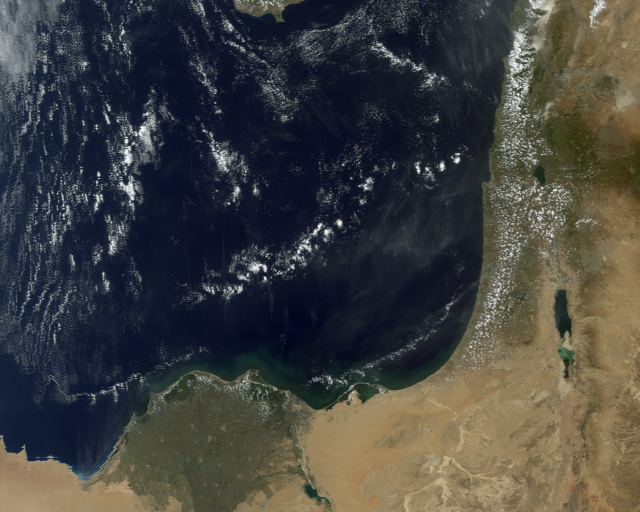
\includegraphics[width=.5\paperwidth]{figs/rgbs/rgb_TC.png}
    \caption{MODIS Truecolor image of my chosen region.}
    \label{title_image}
\end{figure}

\section{Abstract}

In this project I perform K-means and maximum-likelihood pixel classification and subsequent analysis of MODIS L1b data in a region including the Southeast Mediterranean, the Nile River delta, and The Levant. The surface types I focus on are (1) ice clouds, (2) water clouds, (3) vegetation, (4) surface water, and (5) arid ground, though several other surface types were identified by classification. Correlation statistics and spectral analyses of surface classes are provided for each classification result.  I will also use this report as documentation for the Python package I'm developing, as outlined in section \ref{code_comment}.

\clearpage

\section{Code comment}\label{code_comment}

\begin{figure}[h!]
    \centering
    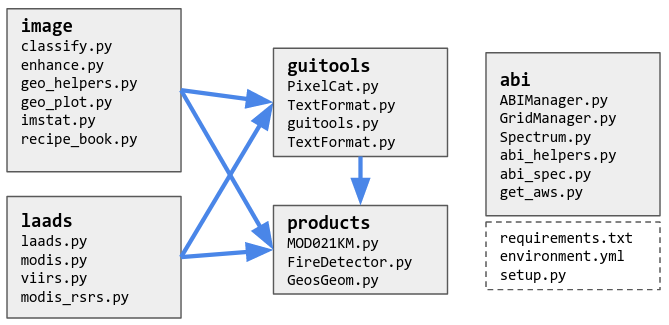
\includegraphics[width=.7\paperwidth]{figs/repo.png}

    \caption{Module layout and dependency graph for my Python package for satellite data acquisition and analysis. The package is organized into modules containing generalized methods for a variety of tasks, as well as several classes for higher-level analysis. In accordance with Python naming convention, class files are capitalized and modules containing only methods are lowercase. My repository can be installed and imported like any other Python package, and is available on GitHub at \url{https://github.com/Mitchell-D/aes670hw2/}}
    \label{repo_diagram}
\end{figure}

One of my major goals for graduate school is to collect code I write for classes and research into a reusable package of software tools with a common architecture and a minimal number of dependencies, which I ultimately want to develop into an ongoing open-source software project. This class has enabled me to make significant headway on my goal, so this report will serve as both a surface analysis of my region and a demonstration of my software. Figure \ref{repo_diagram} shows the layout of my package, which is currently called \hltexttt{aes670hw2} (subject to renaming soon). The package and its dependencies can be installed manually with \hltexttt{pip install /path/to/aes670hw2}, or with \hltexttt{conda-forge} using the included \hltexttt{environment.yml} file. Any of the sub-modules can be imported directly from the package, for example \hltexttt{from aes670hw2 import enhance as enh}.

Software development is a balancing act between usability and re-usability. ``Low-level'' operations like N-dimensional histogram matching must be complicated enough to be useful to specialized tasks without the need for extra infrastructure code, and ``high-level'' methods like getting user input at runtime with a live-rendered RGB must be general enough to be used for a variety of data circumstances. As such, I'm keeping a wide range potential future use cases in mind for each every module, and attempting to separate the methods within each module into a reusable collection of sub-tasks. For instance, \hltexttt{enhance.histogram\_match} is a relatively high-level method that takes two equally-shaped 2d or 3d arrays and histogram-matches the first two axes of the first array to the first two axes of the second array in a provided number of bins. This method is only 19 lines long since it subsequently depends on \hltexttt{enhance.get\_cumulative\_hist}, \hltexttt{enhance.get\_pixel\_counts}, \hltexttt{enhance.norm\_to\_uint}, and other sub-tasks that are re-usable for a variety of other purposes.

I have a long list of future plans for this project, which include developing API wrappers for data sources other than the LAADS DAAC and NOAA AWS buckets, adapting the \hltexttt{products.MOD021KM} class design to support any gridded dataset, and an asynchronous process queue to enable multiple simultaneous OpenCV2 windows. My codebase currently exceeds 7,500 lines of Python, which includes detailed internal documentation for every method. The following tables provide an overview of each module's purpose.

\begin{table}[h!]
    \begin{tabular}{ l p{14cm} }

        \textbf{Module} & \textbf{Purpose} \\\hline

        \hltexttt{products} &
        The \hltexttt{products} module contains three classes: \hltexttt{FireDetector.py}, \hltexttt{GeosGeom.py}, and \hltexttt{MOD021KM.py}. The first is a relatively simple class that executes the fire detection algorithm outlined in (Flasse \& Ceccato, 1996) \cite{flasse1996} with optional custom thresholds, and which only depends on numpy. The second is also a fairly simple but highly generalized class that generates surface latitude/longitude and pixel/sun/sensor trigonometry arrays from basic sun/satellite geometry information for any geostationary satellite. The third, \hltexttt{MOD021KM.py}, is however a very abstract class that provides a wide variety of methods for interfacing with and analyzing MODIS L1b data in the MOD021KM or MYD021KM formats. The class includes static methods for finding, downloading, parsing, calculating, and subsetting a user-provided set of L1b MODIS reflectance and brightness temperature bands to a geographic range. Since MOD021KM objects can be easily created from a L1b HDF, instances of the MOD021KM class are built on and enforce the principles that the underlying band data they are initialized with cannot change, that all contained datasets have an identical shape, and that any band composite recipe can be expressed as a directed tree graph of other composite recipes it depends on, all of which must ultimately terminate with raw band data as a ``leaf node'' argument. This enables the object to repeatably dynamically evaluate a hierarchy of recipe dependencies at runtime. For example, the user may provide the MOD021KM object a \hltexttt{guitools.Recipe} object with an arbitrary function (ie histogram equalization/matching, an analytic function, a 5-band composite), a string label, and a list of band or recipe labels corresponding to the function's arguments. By referencing the label, the new Recipe can be enhanced, histogram-analyzed, rendered as an RGB, or used for threshold selection, classification, fourier analysis, etc. All of these operations can be accessed by calling a single respective method of the MOD021KM instance. The MOD021KM object also contains wrappers on many other methods for GUI selection and enhancement, K-means and migrating means classification, data mask creation/manipulation/comparison, etc, which will be used often throughout this report.
        \\\hline

        \hltexttt{abi} &
        The \hltexttt{abi} module is mostly adapted from one of my old codebases, and isn't integrated with the rest of the package. It contains methods for querying the NOAA AWS Bucket for GOES East and GOES West ABI and GLM data (\hltexttt{get\_aws.py}), subsetting, projecting, and aligning geolocated arrays (\hltexttt{abi\_helpers.py} and \hltexttt{GridManager.py}), and for rendering animations and performing a variety of analyses on time series of ABI data (\hltexttt{ABIManager.py}).
         \\
    \end{tabular}
\end{table}

\begin{table}[h]
    \begin{tabular}{ l p{14cm}}

        \textbf{Module} & \textbf{Purpose} \\\hline

        \hltexttt{image} &
        The \hltexttt{image} module contains sub-modules with methods for performing enhancement and other pixelwise operations on general 2d and 3d arrays (\hltexttt{enhance.py}), plotting continuous and discrete 1d, 2d, and 3d data in a variety of formats with a common configuration style (\hltexttt{geo\_plot.py}), manipulating and interpolating 2d and 3d arrays in multiple coordinate systems (\hltexttt{geo\_helpers.py}), performing histogram analysis, equalization, and matching on arbitrary 2d and 3d arrays (\hltexttt{enhance.py}), applying arbitrary convolutional kernels to arrays with several hardcoded options, running my fast-fourier implementation and applying user-defined frequency masks (\hltexttt{enhance.py}), and contains a variety of hardcoded RGB recipes (\hltexttt{recipe\_book.py}). This module has no dependencies that aren't installed by default in Python \hltexttt{wheel}.
        \\\hline

        \hltexttt{laads} &
        The \hltexttt{laads} module currently consists of 3 main sub-modules: \hltexttt{laads.py}, \hltexttt{viirs.py}, and \hltexttt{modis.py}. The \hltexttt{laads.py} sub-module contains a collection of abstract methods for querying the Earth Observing System's LAADS DAAC archive's REST API, enabling the user to retrieve information about, search for, and download any available product with optional geographic and time constraints. The \hltexttt{viirs.py} and \hltexttt{modis.py} sub-modules use \hltexttt{laads.py} to search for user-specified L1b or L2 swaths at any resolution, and provide methods for parsing their respective data files into a common format consisting minimally of a tuple of requested band arrays, and a list of dictionaries corresponding to each band with meta-information such as conversion coefficients, units, and center wavelengths. These methods also optionally provide coordinate reference, sun/satellite geometry, and terrain information if available.
        \\\hline

        \hltexttt{guitools} &
        The \hltexttt{guitools} module contains the self-titled sub-module \hltexttt{guitools.py} as well as two specialized classes \hltexttt{PixelCat.py} and \hltexttt{TextFormat.py}. The main dependency of this module is the Python wrapper for OpenCV2, which \hltexttt{guitools.py} uses to provide functions to get user input with GUI interfaces and to perform a variety of RGB rendering operations. The sub-module contains GUI methods with a interactive windows prompting the user to select a group of pixels in an image, select a rectangular or circular region of an image, or select a scalar value for the image. The latter method re-renders the image in the window using an arbitrary user-defined function of the array and a scalar variable. This function can be defined to let the user interactively choose contrast, gamma, histogram mean, and value thresholds for an arbitrary scalar array. \hltexttt{guitools.py} also contains lower-level methods for rendering a scalar array as an RGB using linear functions of hue, saturation, and value, returning a PNG as a numpy array, generating an array of unique colors, and getting an RGB array with normally-distributed color histograms according to user-defined means and standard deviations for each channel. The \hltexttt{PixelCat} class is a high-level class offering wrappers on GUI utilities for performing fourier analysis on, enhancing, and selecting pixels from arbitrary RGB arrays, and the \hltexttt{TextFormat} class colors and formats strings using ANSI escape codes for pretty terminal printing.

    \end{tabular}
\end{table}

\clearpage

{\footnotesize
\noindent
\textbf{NOTE:} In order to prevent confusion between class and object methods, I will refer to static class methods with the notation \hltexttt{MOD021KM.static\_method}, and methods that must be called on an instance of the object with the notation \hltexttt{subgrid.object\_method}, where \hltexttt{subgrid} is presumed to be a \hltexttt{MOD021KM} object with all the needed bands loaded. Instances may be initialized with an HDF by calling the static method \hltexttt{subgrid = MOD021KM.from\_hdf(l1b\_hdf, l1b\_bands)}. Existing MOD021KM objects can be stored as a pickle binary file with \hltexttt{subgrid.make\_pkl(pkl\_path)}, and subsequently retrieved from the file with \hltexttt{subgrid = MOD021KM.from\_pkl(pkl\_path)}.
}

\vspace{-.5em}

\section{Data and domain of analysis}\label{data_domain}

\vspace{-.5em}

\begin{figure}[h!]
    \centering
    \begin{center}
        \makebox[\textwidth]{
            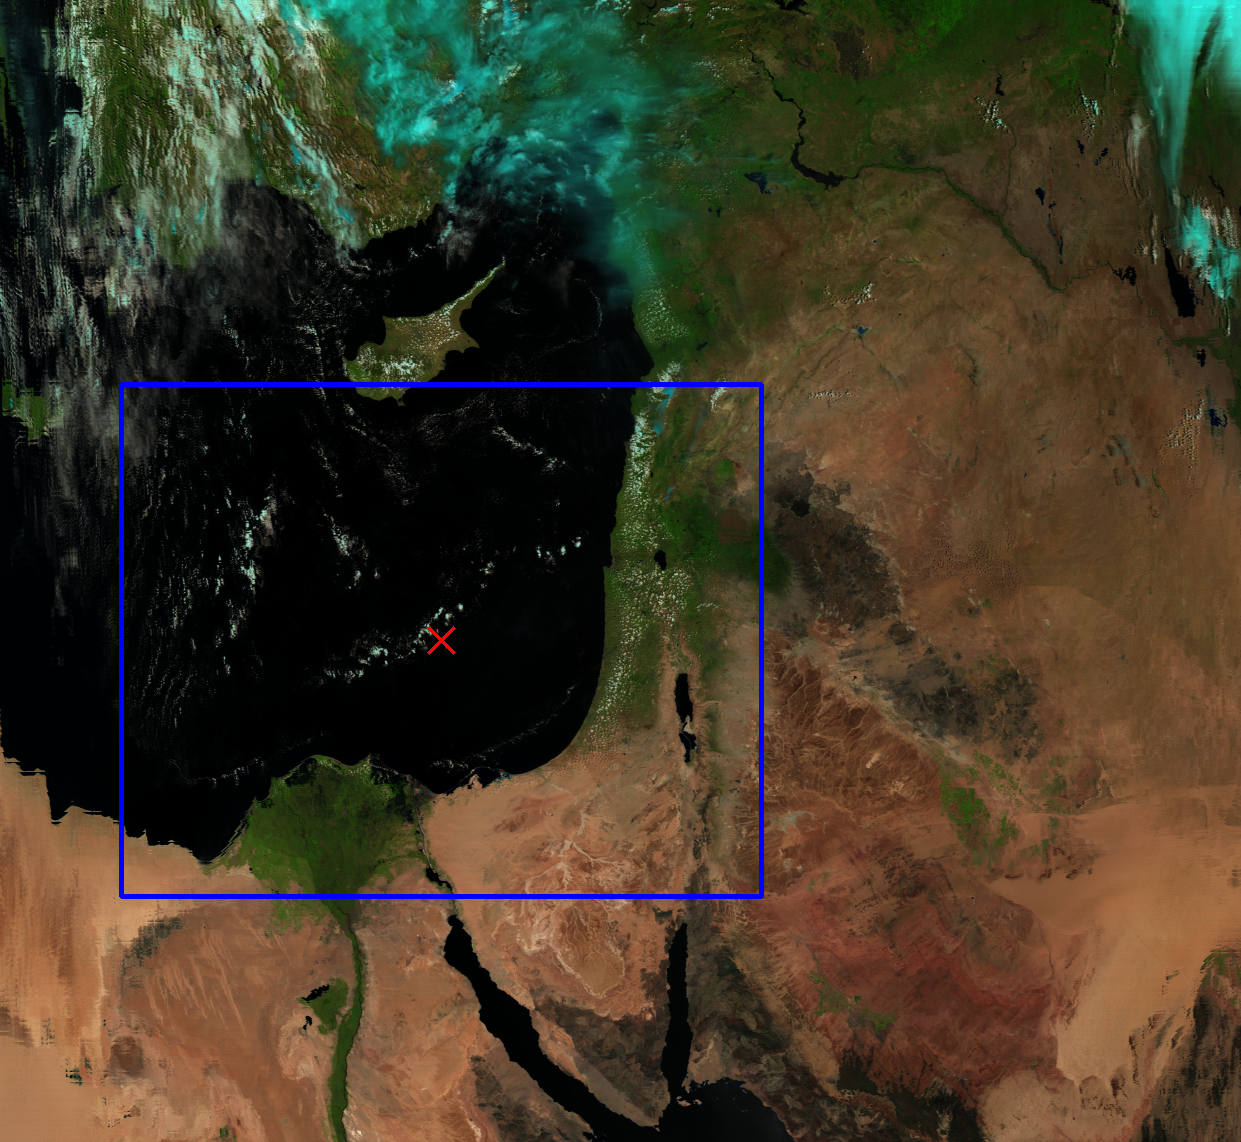
\includegraphics[width=.39\paperwidth]{figs/rgbs/look_DLC.png}
            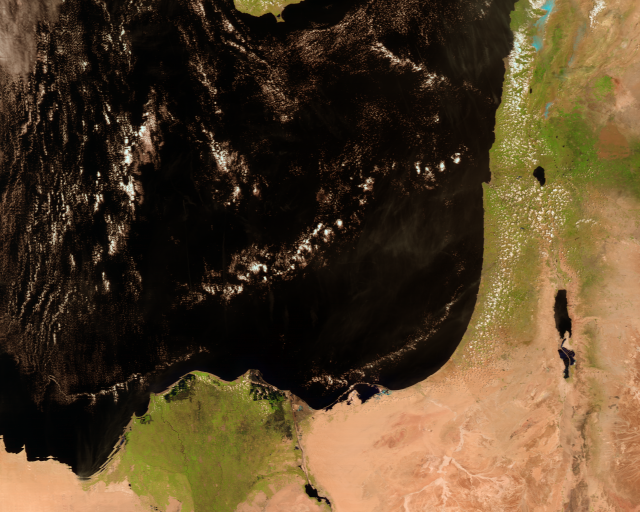
\includegraphics[width=.45\paperwidth]{figs/rgbs/rgb_DLC.png}
        }

        \makebox[\textwidth]{
            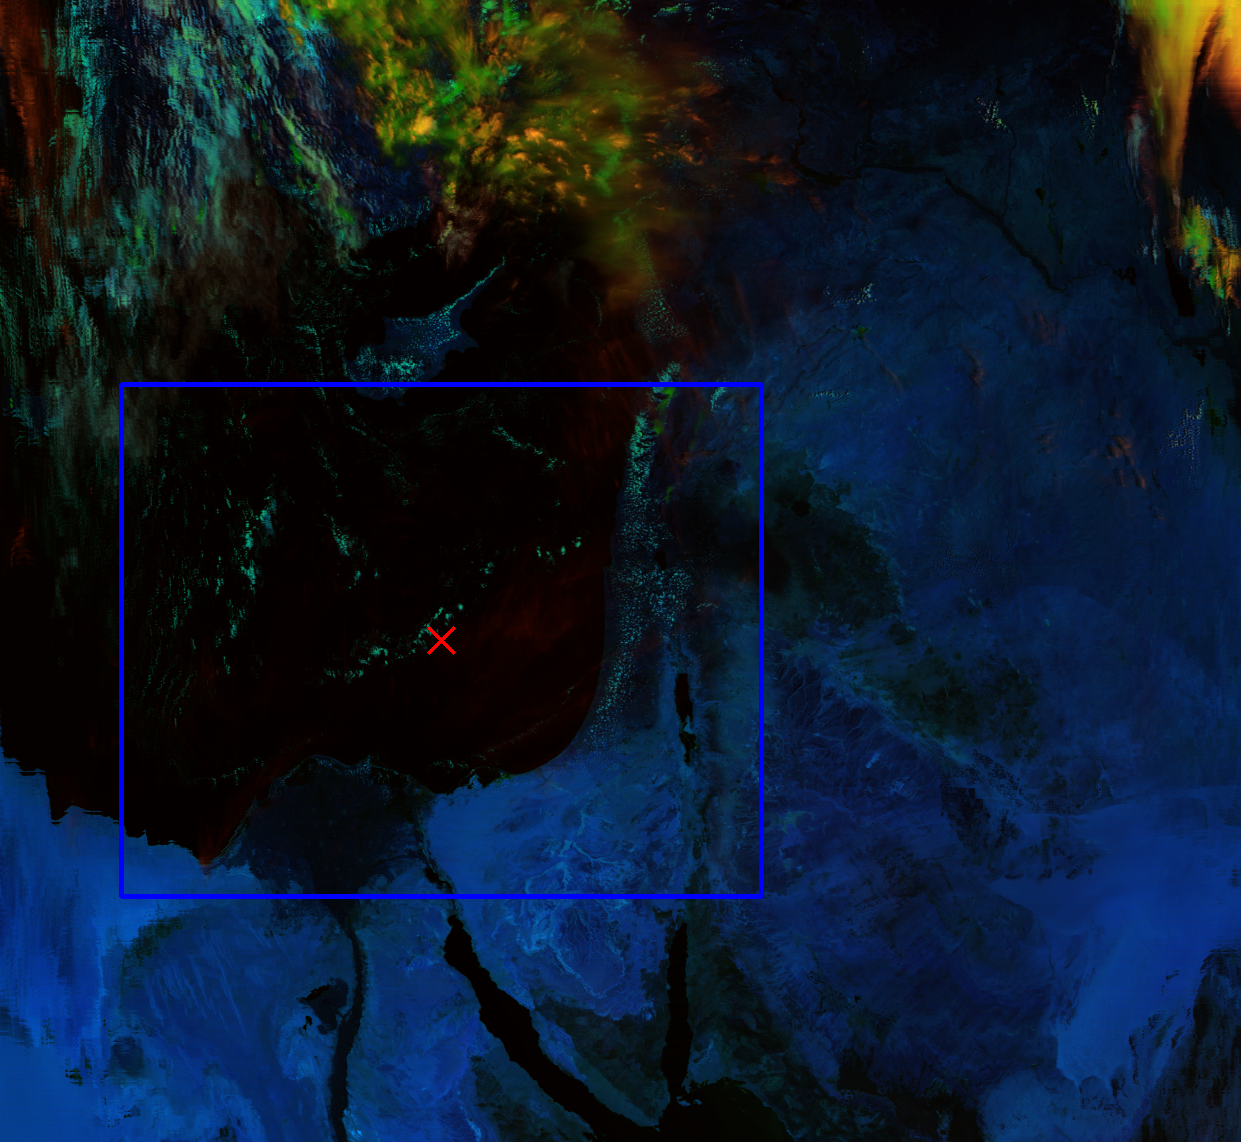
\includegraphics[width=.39\paperwidth]{figs/rgbs/look_DCP.png}
            
\includegraphics[width=.45\paperwidth]{figs/vza_bordered.png}
        }
    \end{center}
    \caption{Top: Natural-color RGBs of a wide view of the location of my region and a focused view of the subgrid I used for analysis, which features the East Mediterranean, the Southern tip of Cyprus, and the Nile River delta on the left, with the Sinai Peninsula and the Levant on the Right. Bottom: Daytime cloud phase RGB composite of a broad view of my region, and a scalar mapping of the viewing zenith angle within my subgrid, which ranges from $0^\circ$ (NADIR; black) to $52^\circ$ (white) from vertical.}
    \label{domain_rgbs}
\end{figure}


\clearpage

Figure \ref{domain_rgbs} provides context on the region that I selected, which is centered on $32.41^\circ$ East, $32.99^\circ$ North and covers a total surface area of $528,689.3km$. The MODIS L1b granule that includes my image was captured by the Terra platform on May 10, 2019 at 0829z, or 10:29am local time in Egypt. I downloaded the L1b data with \hltexttt{MOD021KM.download\_granule}, providing the desired platform, target time, and geographic range of my domain, then initialized a MOD021KM object with the HDF file and a list of all the bands in Table \ref{band_table} using \hltexttt{subgrid = MOD021KM.from\_hdf}.

\begin{figure}[h!]
    \centering

    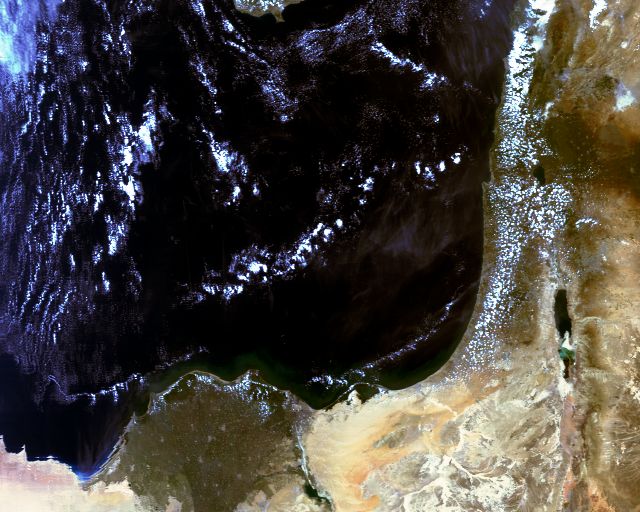
\includegraphics[width=.6\paperwidth]{figs/rgbs/rgb_TCeq.png}

    \vspace{-.9em}

    \begin{center}
        \makebox[\textwidth]{
            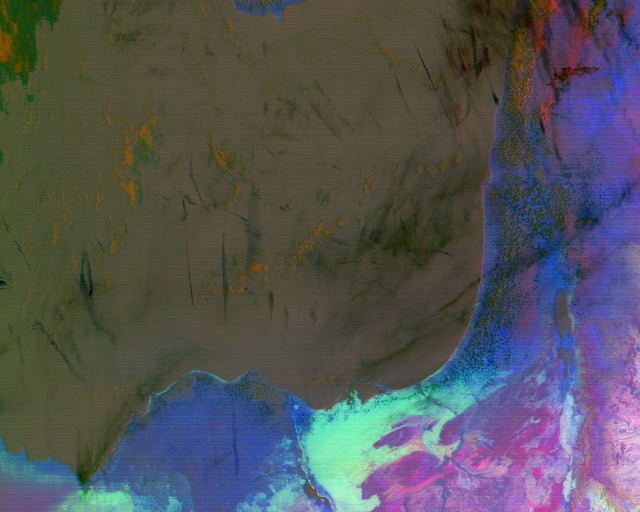
\includegraphics[width=.4\paperwidth]{figs/rgbs/rgb_DUST.png}

            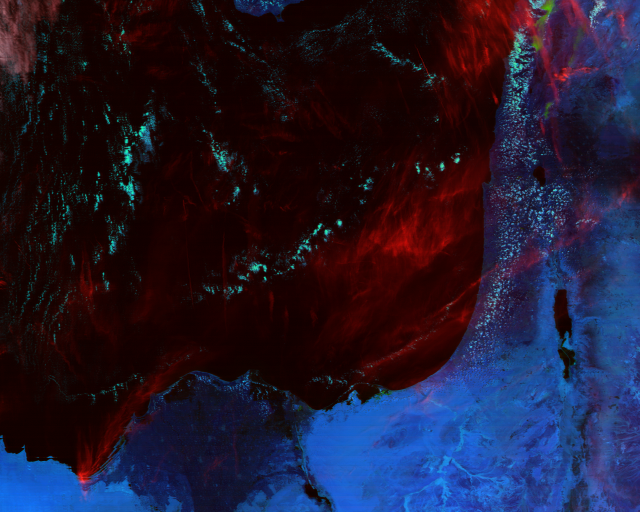
\includegraphics[width=.4\paperwidth]{figs/rgbs/rgb_DCP.png}
        }
    \end{center}

    \caption{Top: histogram-equalized and gamma-enhanced true color RGB. Bottom: gamma-enhanced dust RGB \cite{fuell2016} and daytime cloud-phase RGB \cite{torres2021}. Each of these recipes are loaded by default in \hltexttt{MOD021KM} objects with the labels ``CUSTOMeq,'' ``DUST,'' and ``DCP.'' They were generated with enhancement values manually chosen using the GUI launched by \hltexttt{subgrid.get\_rgb("DUST", choose\_gamma=True)} for each RGB label.}
    \label{region_rgbs}
\end{figure}

\begin{table}[h!]
    \begin{center}
        \renewcommand{\arraystretch}{1.3}
        \begin{tabular}{ l m{10cm} }
            \textbf{Dust RGB channels} & \textbf{Description} \\\hline

            RED=norm($12-11\mu m$) & Cloud and dust optical thickness. Optically thick clouds and clear-sky land surfaces have values near zero, which are normalized to become bright since channel difference values generally range from $-5^\circ C$ to $1^\circ C$. Low values indicate more attenuation by water vapor than $12\mu m$. \\
            GREEN=norm($11-8.6\mu m$) & Cloud particle phase and land surface emissivity. The $8.6$. Water-phase clouds and surfaces with low emissivity have high values. Atmospheric columns with more water vapor absorption will also be tinted green. \\
            BLUE=norm($11\mu m$) & LWIR window for cloud-top and land temperature. \\
        \end{tabular}

        \vspace{.9em}

        \begin{tabular}{ l m{10cm} }
            \textbf{Day-cloud RGB channels} & \textbf{Description} \\\hline

            RED=norm($1.38\mu m$) & Cirrus cloud detection due to strong water vapor attenuation at mid and low layers \\
            GREEN=norm($.64\mu m$) & Visible band for cloud optical thickness \\
            BLUE=norm($1.64\mu m$) & Cloud-phase distinction; Water droplets are reflective, but ice particles strongly absorb. \\
        \end{tabular}
    \end{center}
    \caption{Recipes for false-color RGBs in Figure \ref{region_rgbs}. Note that the sources for these RGB recipes limit data to certain ranges and apply specific gamma enhancements. Those values aren't included here since they can be selected to suit a task at runtime with \hltexttt{subgrid.data("label", choose\_contrast=True, choose\_gamma=True)}.}
    \label{rgb_recipes}
\end{table}

The histogram-equalized true color RGB in Figure \ref{region_rgbs} clearly shows the transition between the barren sandy desert surrounding the Nile Delta and the exposed rock and scrub of the Sinai peninsula, which is corroborated by corresponding light blue/green and magenta surfaces in the dust RGB. The GREEN band of the dust RGB recipe is the $11-8.6\mu m$ LWIR channel difference, which is highly sensitive to the emissivity properties of barren land surfaces \cite{li2012}. Bare stone and soil generally have an emissivity $\epsilon \approx .92$, and sand has an emissivity $\epsilon \approx .89$, which causes the brightness temperature of sand to appear artificially cool in the $8.6\mu m$ band. This inflates the channel difference over sandy surfaces, hence the green hue of that region in the dust RGB.

The $11-8.6\mu m$ channel difference in the dust GREEN channel also contributes more heavily to water-phase clouds than ice-phase clouds due to the much higher emissivity of ice than water, which explains the green tint of low-level water clouds in the RGB. The dust RGB's RED band is the $12-11\mu m$ channel difference, which takes advantage of the additional water vapor attenuation in the $12\mu m$ band to quantify cloud optical depth, as the ratio of surface emissions absorbed at $12\mu m$ to emissions absorbed at $11\mu m$ slightly increases with the amount of water vapor in the atmospheric column. Thus, the tan/orange clouds in the RGB correspond to optically-thick water and mixed-phase clouds, and the dark green pixels correspond to optically-thin and sub-pixel water clouds. The BLUE channel of the dust RGB is simply the $11\mu m$ LWIR window channel, so cirrus clouds are black due to their high emissivity, low optical depth and cold temperature.

The daytime cloud-phase RGB assigns the $1.38\mu m$ cirrus band to RED, the $6.4\mu m$ red band to GREEN, and the $1.64\mu m$ cloud-phase band to BLUE. Since water absorbs very strongly in the NIR range, there is stark contrast between the Mediterranean sea surface, low-level and sub-pixel water clouds, and high-level cirrus clouds. The red streaks throughout the center of the image suggest pervasive thin cirrus contamination over the sea and Israel. Compared to the large-scale daytime cloud phase RGB in Figure \ref{domain_rgbs}, it's clear that these cirrus are very optically thin, which poses challenges in later analysis.

\begin{figure}[h!]
    \centering

    \begin{center}
        \makebox[\textwidth]{
            %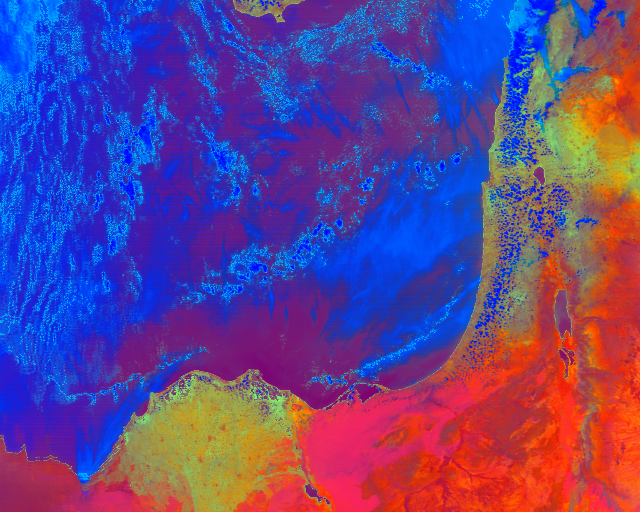
\includegraphics[width=.45\paperwidth]{figs/rgbs/rgb_CUSTOMeq.png}

            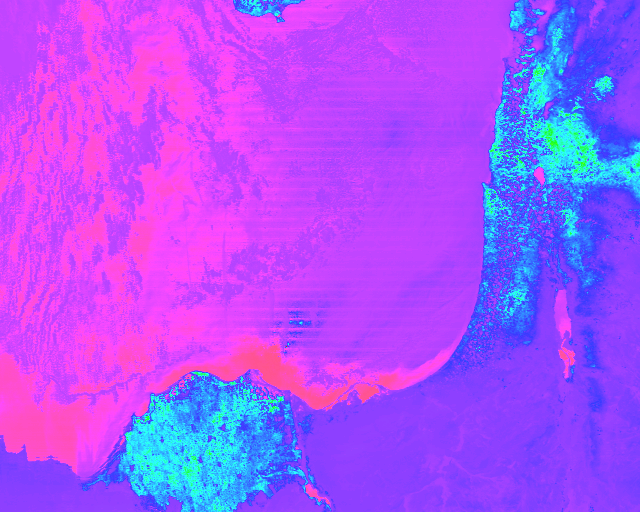
\includegraphics[width=.4\paperwidth]{figs/hsv/gamma_ndvi.png}

            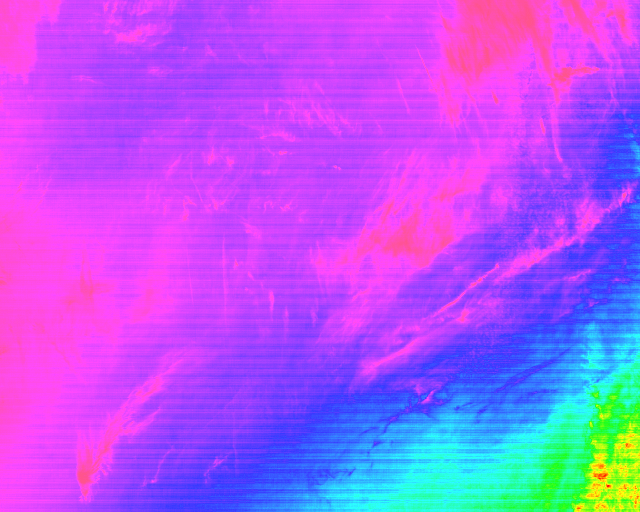
\includegraphics[width=.4\paperwidth]{figs/hsv/gamma_hsv_28.png}
        }
    \end{center}

    \vspace{-.9em}

    
\includegraphics[width=.3\paperwidth]{figs/hsv/cbar.png}

    \caption{Left: gamma-enhanced heatmap of NDVI (using $.86\mu m$ NIR and $.64\mu m$ RED bands). Right: gamma-enhanced heatmap of MODIS band 28 ($7.3\mu m$) brightness temperatures. Both images are normalized to the scale of the color bar below low values in magenta and high values in red. These were generated by \hltexttt{geo\_plot.generate\_raw\_image} using RGBs from \hltexttt{guitools.scal\_to\_rgb}, for example: \hltexttt{guitools.scal\_to\_rgb(subgrid.data("ndvi",choose\_gamma=True))}. Hue, saturation, and value ranges for the RGB-mapped scalar array can be optionally provided.}
    \label{hsv_ndvi_28}
\end{figure}

The left image in Figure \ref{hsv_ndvi_28} shows a heatmap of vegetation on the banks of the Mediterranean, which captures the arid climate of the Sinai penninsula, the sparse vegetation of the Jordanian highlands, and the highly-vegetated Nile Delta and Levant regions, as well as the southern tip of Cyprus. The right image shows the $7.175-7.475\mu m$ mid-level water vapor band, which features cold brightness temperatures indicating a steep gradient of vapor content increasing to the Northwest over the sea. Water vapor is especially concentrated along the West edge of the region, which is further occluded by sub-pixel clouds and panoramic distortion as the true color RGB in Figure \ref{region_rgbs} and viewing zenith angle render in Figure \ref{domain_rgbs} suggest.

Both of the images in Figure \ref{hsv_ndvi_28} also show the effects of data striping, perhaps due to faulty cross-calibration of data from adjacent scan mirrors. Unfortunately bands 2, 5, 6, 7, 21, 26, 27, 28, and 33 were all somewhat affected by the striping. Although this poses some challenges in classification, enough bands were salvagable or intact to achieve reasonable results. Table \ref{band_table} shows the range of bands I chose for initial analysis. The 11 bands I ultimately selected for classification tasks after experimenting with K-means in Section \ref{section_km} are marked with an asterisk in the table.


\begin{table}[h!]
    \centering
    {
        \renewcommand{\arraystretch}{1.3}
        \begin{tabular}{ >{\centering\arraybackslash} m{1cm} >{\centering\arraybackslash} m{3cm} m{10cm} }
            \textbf{Band} & $\boldsymbol{\lambda}$ ($\boldsymbol{\mu} \boldsymbol{m}$) & \textbf{Justification} \\\hline
            03* & $.459-.479$ & Blue band: True color BLUE; sensitive to aerosols. \\\hline
            10 & $.483-.493$ & Teal/blue: ocean color and general reflectivity. \\\hline
            04* & $.545-.565$ & Green: Vegetation, NDSI, and true color GREEN. \\\hline
            01* & $.620-.670$ & Near-red: land surface properties, true color RED. \\\hline
            02* & $.841-.876$ & NDWI for surface water, and NDVI due to the high reflectance of chloryphyll in the near-infrared range. \\\hline
            16 & $.862-.877$ & Ocean color and aerosol distinction \\\hline
            19* & $.916-.965$ & Partial H$_2$O absorption, for column moisture estimates. \\\hline
            05* & $1.230-1.250$ & Cloud/aerosol optical depth and land surface properties. \\\hline
            26* & $1.360-1.390$ & Steep H$_2$O absorption curve for high cloud reflectance. \\\hline
            06 & $1.628-1.652$ & Snow/ice band: indeces of refraction differ between ice and liquid-phase water. Water clouds are reflective and ice clouds strongly absorb. \\\hline
            07 & $2.106-2.155$ & Cloud and aerosol particle size band: small particles are similar in size to $2.2\mu m$, so they are readily reflected via Mie scattering. Large particles absorb incident light \cite{platnick2018}. \\\hline
            20* & $3.660-3.840$ & SWIR ``Magic band'': solar reflectance as well as infrared emissions. Useful for a variety of derived products, especially for fire detection.  \\\hline
            21 & $3.929-3.989$ & Infrared-biased narrow SWIR for cloud and land surface temperature. Spans the edge of a CO$_2$ absorption line. \\\hline
            27 & $6.535-6.895$ & High infrared cloud features due to very strong H$_2$O absorption. \\\hline
            28* & $7.175-7.475$ & Mid-level infrared cloud properties due to moderate attenuation by atmospheric water vapor. \\\hline
            29* & $8.400-8.700$ & Infrared cloud phase and land features, as well as atmospheric column water content from weak vapor absorption. Sensitive to the emissivity of surfaces. \\\hline
            31* & $10.780-11.280$ & Clean long-wave window band: very little atmospheric absorption, so the actual temperature of surfaces can be estimated with knowledge of their emissivity.  \\\hline
            32 & $11.770-12.270$ & LWIR window: observed temperatures are slightly sensitive to artificial cooling depending on the altitude of the pixel surface. \\\hline
            33 & $14.085-14.385$ & Dirty LWIR: much stronger attenuation by water vapor makes it easy to characterize column vapor content. \\\hline
            \multicolumn{3}{m{14cm}}{* \textit{Starred bands indicate the subset chosen for use in K-means and maximum-likelihood classification. All bands were used for analysis.}} \\
        \end{tabular}
    }
    \caption{Band number, spectral response range, and purpose of every MODIS band I used for analysis.}
    \label{band_table}
\end{table}

\clearpage

\section{My custom RGB}\label{section_custom_rgb}


\begin{figure}[h!]
    \centering
    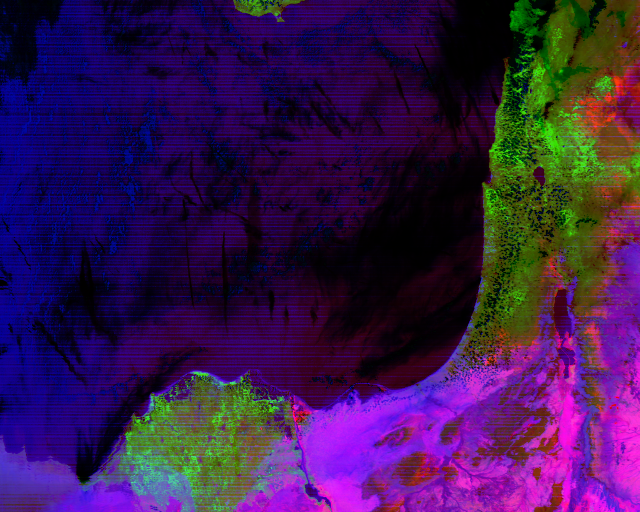
\includegraphics[width=.8\linewidth]{figs/rgbs/rgb_CUSTOMhistgamma.png}

    \caption{My custom RGB, enhanced to reveal land surface temperature and emissivity, vegetation density, atmospheric vapor content, and to mask thin clouds.}
    \label{custom_rgb}
\end{figure}

\begin{table}[h!]


    \begin{center}
        \makebox[\textwidth]{
            \renewcommand{\arraystretch}{1.3}
            \begin{tabular}{ l m{4.5cm} m{9cm} }
                \multicolumn{2}{l}{\textbf{Custom RGB channels}} & \textbf{Description} \\\hline

                RED & \hltexttt{\small gamma(hist(norm(R)))} \footnotesize{R$=$T$_B(11\mu m)$}
                & LWIR window band, histogram-matched to a normal distribution with $\mu=.5$ and $\sigma=.2$. Saturates cold temperatures to indicate land and sea surface temperature, distinguish land from clouds, and enhance land features. \\
                GREEN & \hltexttt{\small gamma(hist(norm(G)))} \footnotesize{G$=$NDVI$|_0^1$}
                & Subsetted and normalized NDVI, histogram-matched to a normal distribution with $\mu=.3$ and $\sigma=.2$. Saturates clouds and water near zero and stratifies the brightness histogram over high brightness values in the vegetation range. \\
                BLUE & \hltexttt{\small gamma(hist(norm(B)))} \footnotesize{B=T$_B(11\mu m) \div $T$_B(8.6\mu m)$}
                & Normalized $11 \div 8.6\mu m$ band ratio, histogram-matched to a normal distribution with $\mu=.5$ and $\sigma=.3$. Sensitive to land surface emissivity and atmospheric vapor content. \\
        \end{tabular}
        }
    \end{center}

    \vspace{-1em}

    \caption{Custom RGB recipe. Normal distribution values are selected to provide baseline histograms, which can be shifted with gamma enhancement to accentuate the features needed for a specific task.}
    \label{custom_recipe}
\end{table}

\clearpage

\begin{figure}[h!]
    \centering

    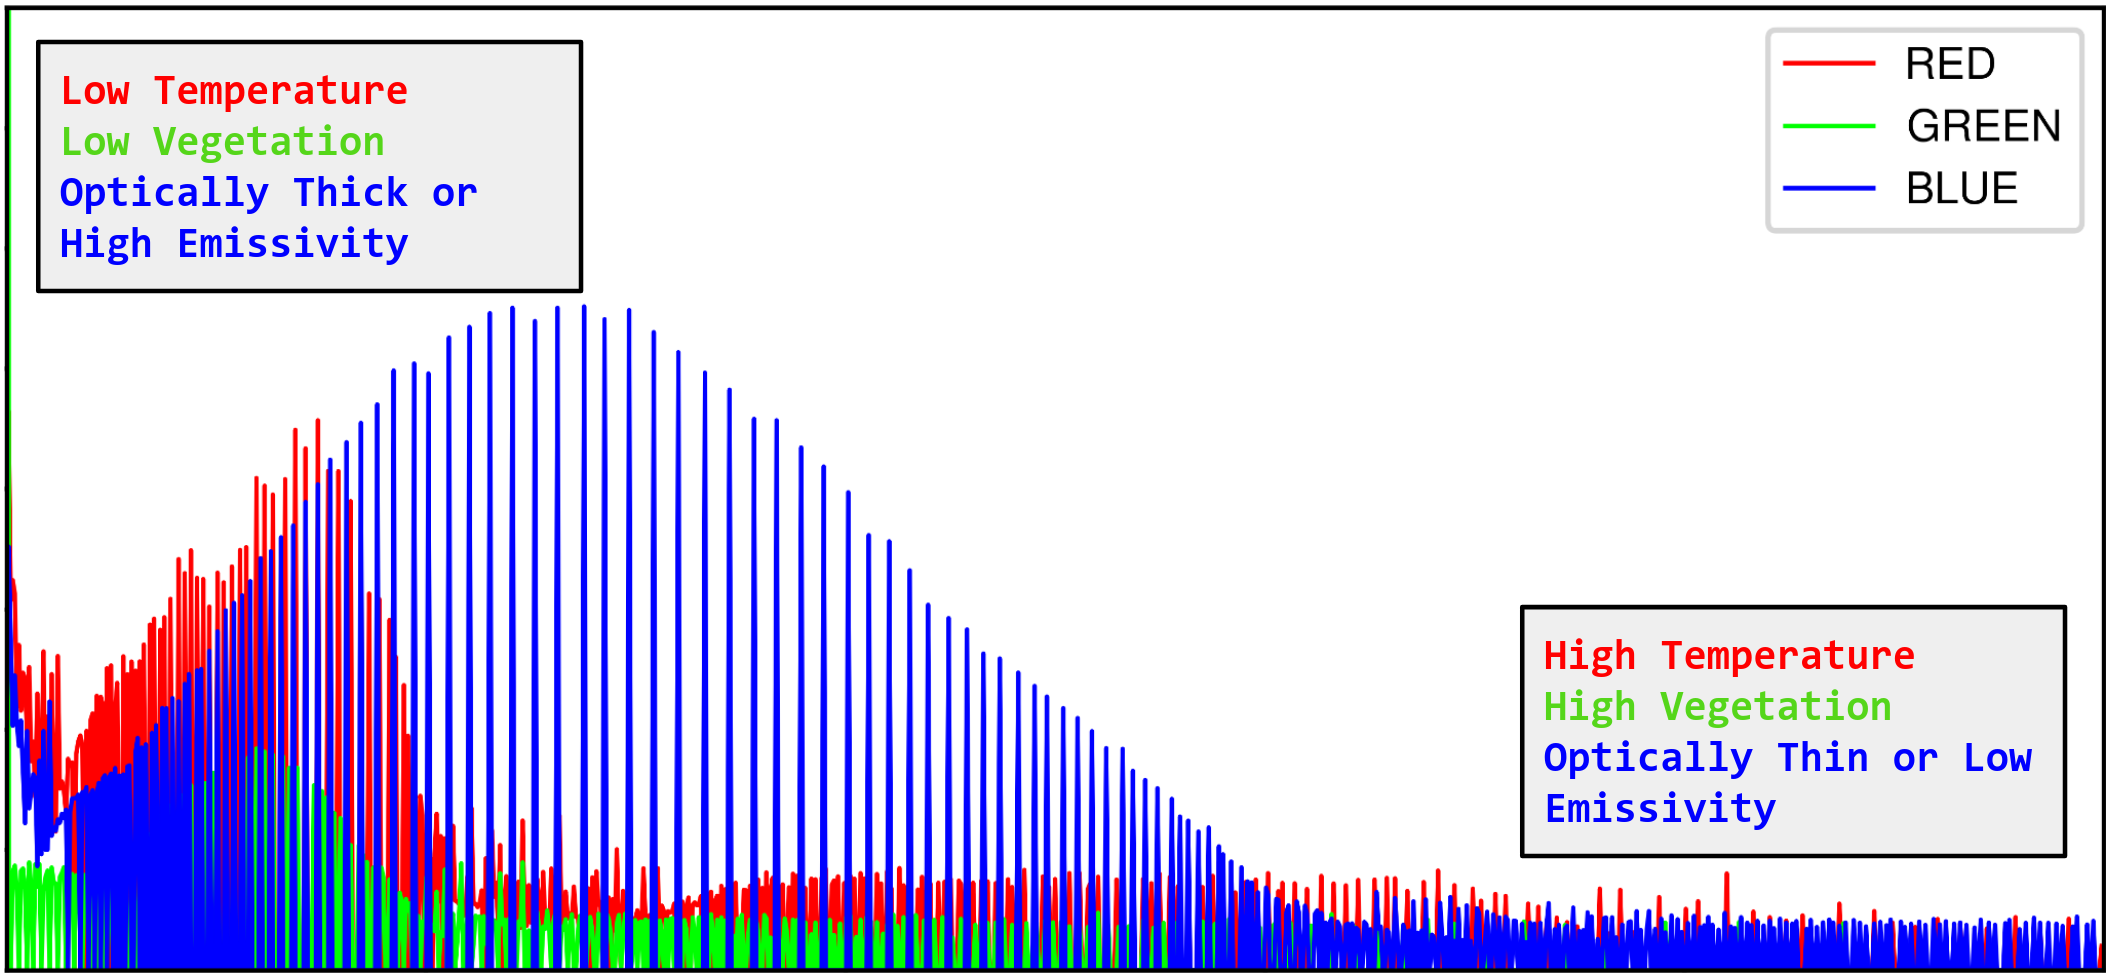
\includegraphics[width=.8\linewidth]{figs/spectra/custom_matched_annot.png}

    \vspace{-1em}
    \begin{center}
    \makebox[\textwidth]{
        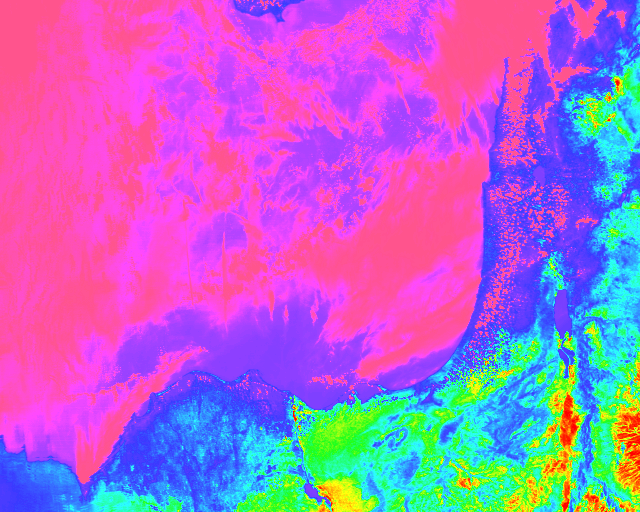
\includegraphics[width=.24\paperwidth]{figs/rgbs/rgb_CUSTOMhistgamma_RED.png}
        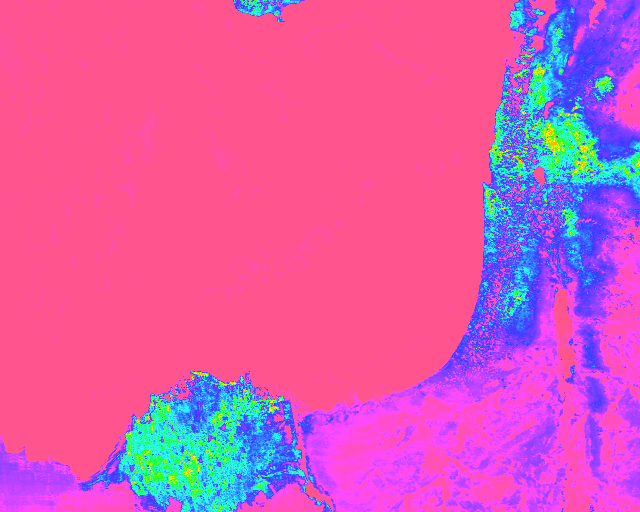
\includegraphics[width=.24\paperwidth]{figs/rgbs/rgb_CUSTOMhistgamma_GREEN.png}
        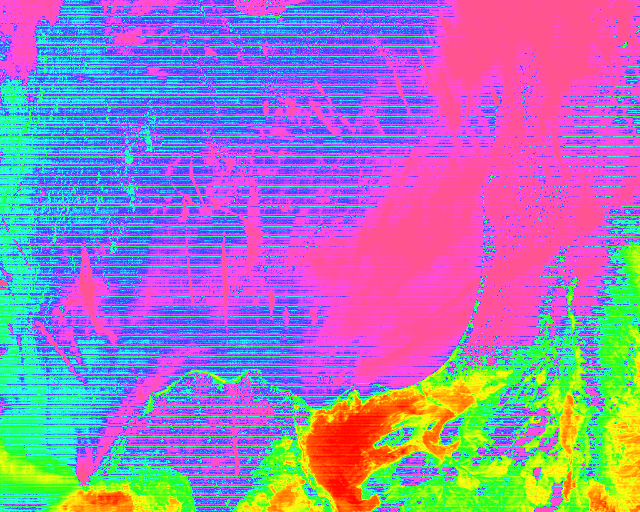
\includegraphics[width=.24\paperwidth]{figs/rgbs/rgb_CUSTOMhistgamma_BLUE.png}
    }
    \end{center}

    \vspace{-.9em}

    
\includegraphics[width=.5\linewidth]{figs/rgbs/cbar_hist.png}

    \caption{Normalized brightness frequency histogram, and heat map renders of each color component's scalar array with a colorbar demonstrating the data distribution from minimum (magenta) to maximum (red).}
    \label{custom_components}
\end{figure}

\vspace{-.8em}

In order to further investigate the features identified in Section \ref{data_domain}, I developed an RGB sensitive to vegetation, precipitable water vapor (PWV), land surface and cloud-top temperatures (LST, CTT), and land surface emissivity (LSE). As outlined in Table \ref{custom_recipe}, the RED band is the longwave infrared window, which corresponds directly to LST and CTT, and serves as a reference point for BLUE channel values. The GREEN band is the NDVI with the $.86\mu m$ and $.64\mu m$ bands (1 and 2), with high and low values cropped to the $[0,1]$ range, then normalized, which saturates barren land, clouds, and water and enhances vegetation density. The BLUE band is the $11 \div 8.6\mu m$ longwave infrared band ratio, the behavior of which is the most difficult to intuit since bright values correspond to different phenomena on land and in the atmosphere.

On one hand, in the atmosphere, the BLUE band ratio is large where $8.6\mu m$ band brightness temperatures are suppressed by water vapor as discussed in Section \ref{data_domain}. This is apparent at the edges of water clouds, in regions with sub-pixel clouds, and in regions with high PWV. Optically thick (and especially high-altitude) clouds have similar brightness temperatures in both bands, and as such have low ratio values. In clear-sky regions, on the other hand, the BLUE band ratio is dominantly sensitive to LSE. The inverse Planck function \hltexttt{modis.get\_modis\_data} uses to calculate brightness temperatures from infrared radiance implicitly assumes that the emissivity of incident surfaces is $\epsilon = 1$. Since the $8.4-8.7\mu m$ band occupies a spectral range right on the steep low-wavelength edge of the $T\approx 300K$ blackbody emission curve, it is more sensitive to error in this assumption. Thus low-emissivity surfaces like sand ($\epsilon \approx .89$) appear brighter in the ratio than high-emissivity surfaces like vegetation ($\epsilon \approx .94$).

Both of the phenomena influencing the BLUE band ratio are ultimately the consequence of changes in emissivity among surfaces, as atmospheric layers with a low optical depth equivalently have low emissivity. Nonetheless, my RGB's property that low LSE and high PWV both correlate with high BLUE brightness values can make interpretation challenging. For example in Figure \ref{custom_rgb}, the sandy region Southwest of the Nile Delta appears artificially more blue than the similarly sandy region at the East edge of the delta due to the increased presence of PWV from the moist airmass seen in Figure \ref{hsv_ndvi_28}.

I created the custom RGB featured in Figure \ref{custom_rgb} by adding new scalar recipes for each channel, for example: \hltexttt{subgrid.add\_recipe("LWrat",(29,31),lambda a,b:norm(b/a))}, then an RGB recipe with arguments for each channels using \hltexttt{subgrid.add\_rgb\_recipe}. Next, I called \hltexttt{guitools.get\_normal\_rgb} to generate an RGB array with the same shape as my data, which contains normally-distributed scalar values in each 2d channel corresponding to the means and standard deviations specified in Table \ref{custom_recipe}, which are sampled in the $[0,1]$ range. Then I histogram-matched my custom RGB recipe to the normally-distributed RGB array with \hltexttt{subgrid.histogram\_match}, adding the data array to my \hltexttt{subgrid} object with \hltexttt{subgrid.add\_rgb\_data("CUSTOMhist", rgb)}. Finally, I shifted the brightness histograms to distributions convenient for land-surface analysis by calling \hltexttt{subgrid.get\_rgb("CUSTOMhist",choose\_gamma=True)}.

Figures \ref{custom_rgb} and \ref{custom_components} are the results of executing this procedure for a single RGB. The spectral distribution in Figure \ref{custom_components} was generated by calling \hltexttt{subgrid.rgb\_histogram\_analysis} with the RGB's data label ``CUSTOMhist''. Each channel heatmap in the figure was created by generating an RGB with \hltexttt{guitools.scal\_to\_rgb} using custom HSV range parameters, then generating images with \hltexttt{gui\_plot.generate\_raw\_image}.

 Low-density vegetation appears brown due to mid-brightness contributions from each channel since partially-vegetated land surfaces are generally warmer, have a lower NDVI, and have a lower total emissivity than heavily vegetated ares. The same logic applies to high and low-vegetation regions since NDVI strongly correlates with surface emissivity as outlined in (Van De Griend, 2007)\cite{griend2007}. After consulting a geographic atlas \cite{compactworldatlas}, I realized that the red regions in Jordan and Syria correspond very closely to the Sinai mountain ridge and the Judaean mountains. The geology of this region suggests that these areas mostly consist of exposed and fragmented limestone, which has an emissivity around $\epsilon=.95$. The surrounding pink and purple regions are dominantly loamy soil and exposed sandstome, which have emissivities around $\epsilon=.92$ \cite{compactworldatlas}\cite{mineo2021}\cite{bentor1980}, hence the contribution from the BLUE channel.

The blue-tinted regions over the Mediterranean on the left of the Figure \ref{custom_rgb} deomonstrate the PWV of the moist air mass over the Mediterranean, as discussed. Optically thick water and dense ice clouds appear black over land and water appear due to their high emissivity and low temperatures in the LWIR window band. The top right of the image features thin cirrus clouds over a vegetated surface, which appear blue/green due to their low emissivity and the diffusion of near-infrared reflectance from vegetation through the cloud. This is an additional example of the interpretation challenge mentioned previously.

\clearpage

\section{Data thresholding}

\begin{figure}[h!]
    \centering

    \begin{center}
        \makebox[\textwidth]{
            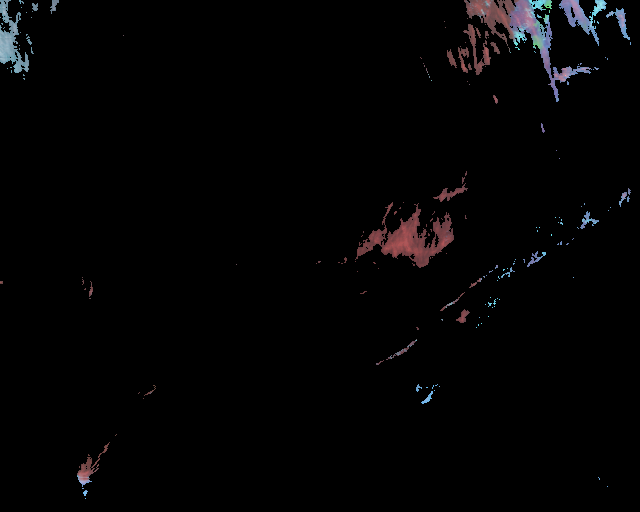
\includegraphics[width=.3\paperwidth]{figs/masks/mask_ice_cloud.png}
            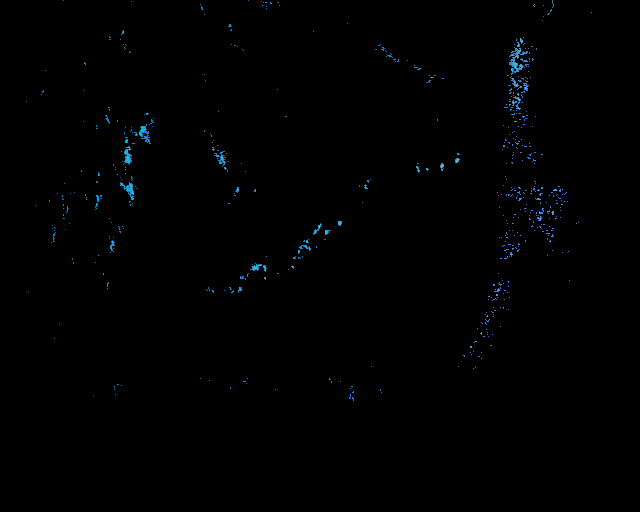
\includegraphics[width=.3\paperwidth]{figs/masks/mask_water_cloud.png}
        }

        \vspace{.2em}

        \makebox[\textwidth]{
            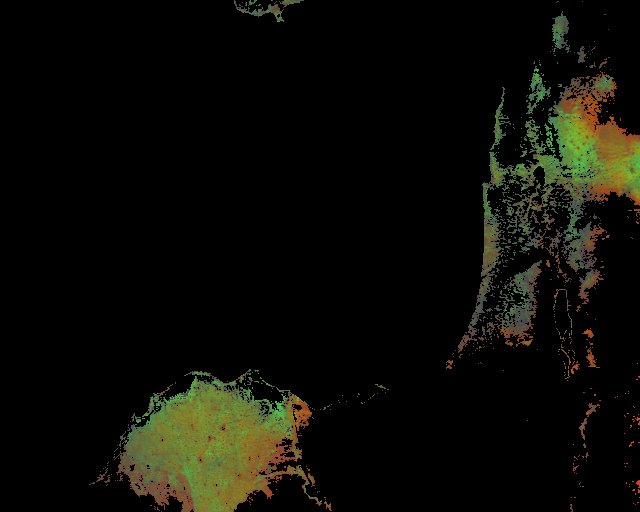
\includegraphics[width=.3\paperwidth]{figs/masks/mask_vegetation.png}
            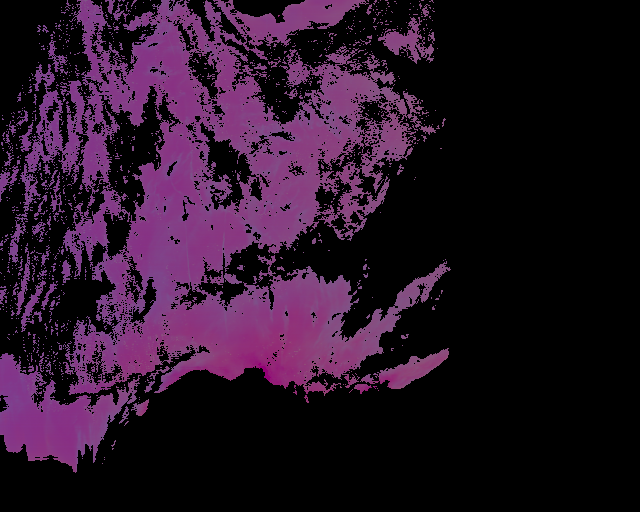
\includegraphics[width=.3\paperwidth]{figs/masks/mask_water.png}
            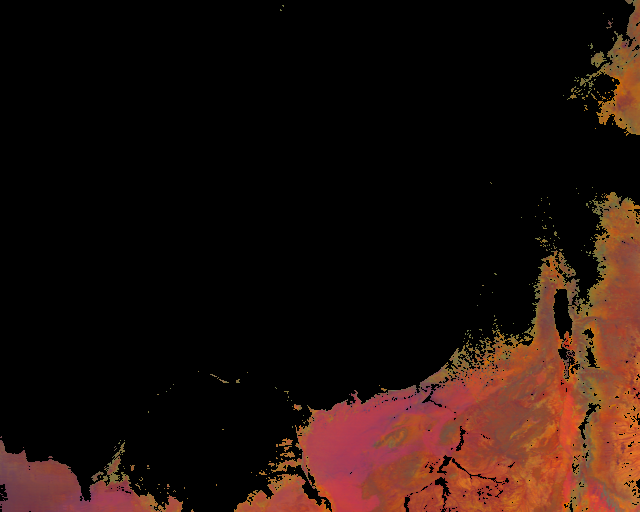
\includegraphics[width=.3\paperwidth]{figs/masks/mask_arid.png}
        }
    \end{center}

    \caption{Masks selected by thresholding procedure. Top: ice cloud and water cloud surface classes. Bottom: vegetation, water, and arid surface classes. Unmasked data values are histogram-matched to the primary RGB used to isolate the class.}
    \label{thresh_masks}
\end{figure}

In order to isolate the 5 surface types I'm analyzing, I manually selected valid reflectance and brightness temperature ranges with \hltexttt{subgrid.get\_mask} for a series of bands and RGB recipes. This method launches a GUI interface with a trackbar input form and an image that is rendered with a callback loop depending on the value of the input. For each channel of each RGB in my procedure, I used the trackbar to select a lower and upper bound for the mask. After data ranges for a surface class were determined, I histogram-matched the in-range values to the RGB that best accentuates the surface type using \hltexttt{subgrid.histogram\_match}. Figure \ref{thresh_masks} shows the results, which rule out pixels that were out of bounds for any channel in any image used for thresholding the class.

Histogram-matched surface class masks are useful for interpretation because the histogram matching process spreads out brightness values of RGB channels with high variance for data values in the class. For example, the vegetation mask was histogram-matched to my custom RGB. There are a wide range of plant densities visible in this mask due to the variability in the RED (LWIR) and GREEN (NDVI) channels of my custom RGB. The water mask, which was also matched to my RGB, features a bright region just Northeast of the Nile Delta, which corresponds to warmer regions in the RED (LWIR) channel from a relative lack of sub-pixel clouds and atmospheric moisture, as suggested by the $7.3\mu m$ channel rendering in Figure \ref{hsv_ndvi_28}, and the relatively high temperature and low emissivity in this region indicated by Figure \ref{custom_components}'s RED and BLUE channels.

\clearpage

\noindent
\textbf{Thresholding methodology}

\begin{enumerate}
    \item{The \textbf{ice cloud} class is selected with upper and lower bounds on each chanel of the daytime cloud-phase RGB, which includes the $1.38\mu m$ cirrus band for middle and low-cloud masking as well as the $1.64\mu m$ cloud-phase band to rule out water clouds.}
    \item{The \textbf{water cloud} mask is selected by masking ice clouds with the daytime cloud-phase RGB, and land surfaces with my custom RGB.}
    \item{The \textbf{arid land} mask is selected using my custom RGB, which was specifically enhanced to accentuate land features and vegetation as discussed in Section \ref{section_custom_rgb}.}
    \item{The \textbf{vegetation} mask is also selected with my custom RGB, using a different gamma enhancement after histogram-matching which is selected manually to better expose vegetation. I used my own discretion to set boundaries where vegetation became too sparse.}
    \item{The \textbf{water} class is the most difficult to isolate due to the abundance of PWV and sub-pixel clouds in my case. Optically thick clouds and most land are masked with my custom RGB, then coastlines are masked with the $8.6-2.1\mu m$ NIR water index (NDWI). Finally, all prior masks are negated from the water mask.}
\end{enumerate}

\begin{table}[h!]
    \centering
    \begin{tabular}{c|cccccc}
        & Ice Cloud & Water Cloud & Vegetation & Water & Arid \\
        \hline
        Pixel Count & 10,094 & 2,227 & 36,614 & 96,730 & 68,922\\
        Area (km$^2$)& 14,426 & 3,221 & 48,431 & 181,319 & 85,435\\
    \end{tabular}
    \caption{Area and quantity of thresholded pixel classes.}
    \label{thresh_areas}
\end{table}

Table \ref{thresh_areas} shows the number of pixels and approximate surface area of each of the classes derived from thresholding. Areas were calculated for each surface type by passing the 2d boolean array returned by \hltexttt{subgrid.get\_mask} to the \hltexttt{subgrid.area} method, which returns the sum of the surface areas of unmasked pixels by calculating the pixelwise panoramic distortion with the viewing zenith angle array (\hltexttt{subgrid.data("vza")}). This table makes clear that water and arid land dominate the region, followed by vegetated land surfaces.

Ice clouds and water clouds are under-represented because I intentionally chose restrictive thresholds for these classes. Clouds in general were difficult to threshold due to the scarcity of vapor bands uncorrupted by striping, the wide range of PWV values in my region, and the presence of mixed-phase clouds over the Mediterranean. For example, note the light blue mid-level water-phase clouds present on the right side of the ice cloud mask in Figure \ref{thresh_masks}. These inhabit a region with low precipitable water vapor and a very thin cirrus layer, and as such weren't masked with a lower bound on LWIR brightness temperature or the $1.37\mu m$ cirrus band. Since I will sub-sample my thresholded classes to use as training samples for maximum-likelihood classification, I wanted to leave as little ambiguity as possible in each class' spectral signature.

\clearpage

\noindent
\textbf{Thresholded surface classes: spectral response and error}


\begin{figure}[h!]
    \centering

    \begin{center}
        \makebox[\textwidth]{
            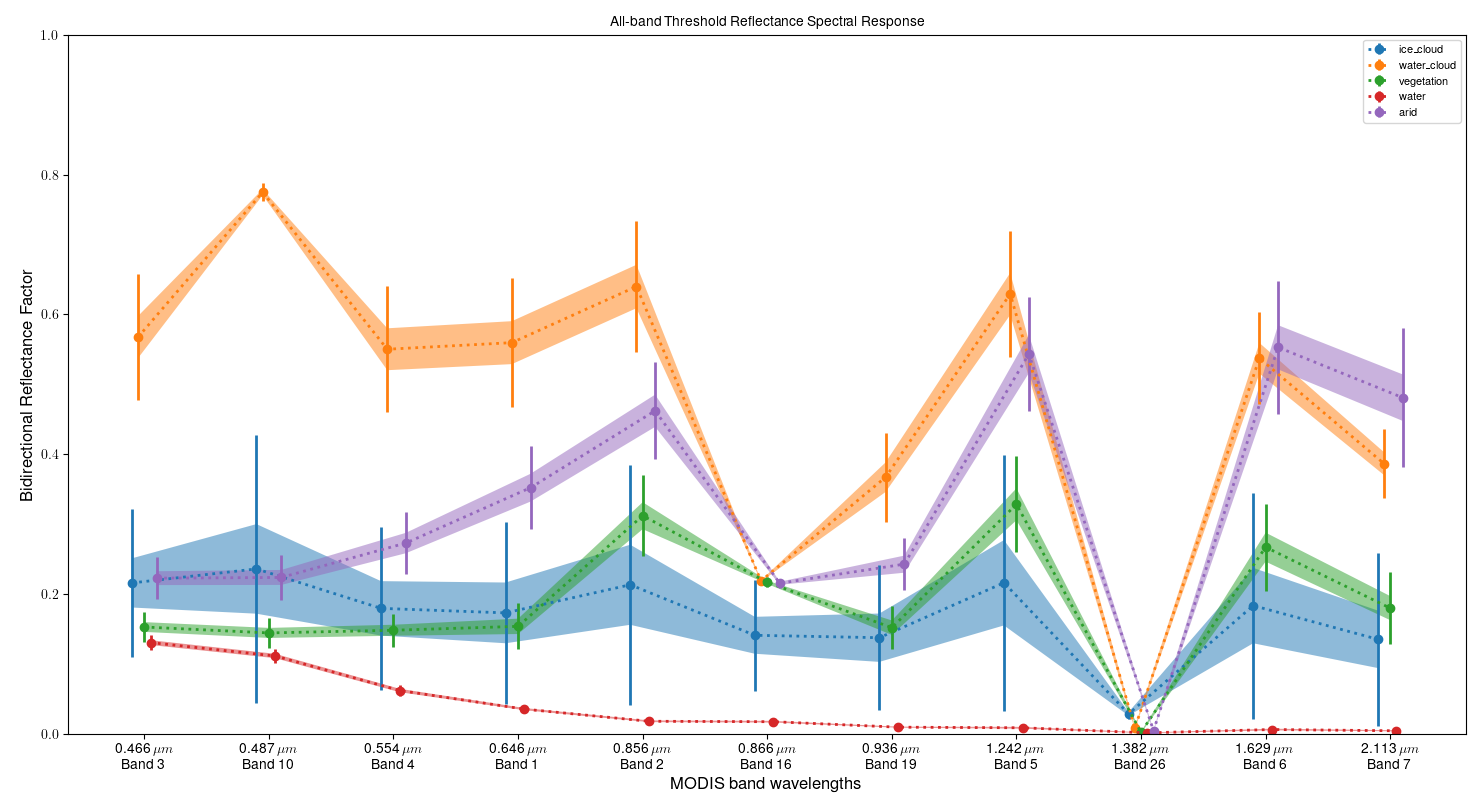
\includegraphics[width=.85\paperwidth]{figs/spectra/ref_thresh_all_crop.png}
        }
        \makebox[\textwidth]{
            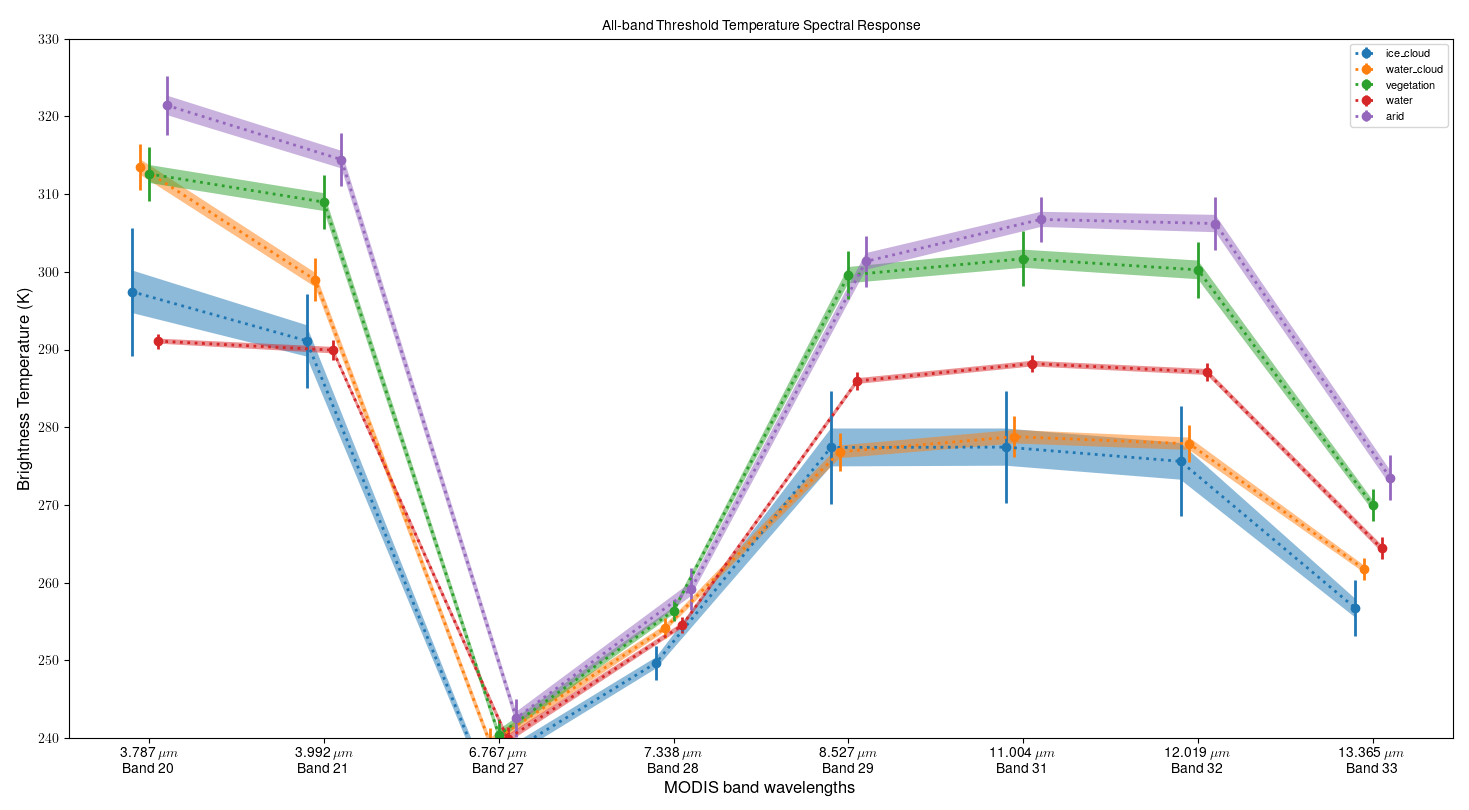
\includegraphics[width=.85\paperwidth]{figs/spectra/temp_thresh_all_crop.png}
        }
    \end{center}

    \caption{Reflective and thermal spectral response of each threshold-derived surface class. Each data point is the mean value of the class at that wavelength with $1-\sigma$ error bars and $\frac{1}{3}-\sigma$ shaded regions. These plots were generated with the surface class masks from the thresholding procedure using \hltexttt{subgrid.spectral\_analysis}, which is a wrapper on the \hltexttt{geo\_plot.stats\_1d} function.}
    \label{thresh_spectra}
\end{figure}

\clearpage

\begin{table}[h!]
\centering
\begin{tabular}{C|C|C|CCCCCCC}

\lambda & \mu & \sigma & \multicolumn{7}{c}{Reflectance Covariance $(\times10^{4})$} \\

\hline
\multicolumn{10}{c}{Ice Cloud} \\
\hline
0.466 & 0.216 & 0.105 & 111.3 & 118.5 & 125.2 & 138.0 & 88.5 & 135.7 & 0.5 \\
0.554 & 0.180 & 0.117 & 118.5 & 136.2 & 150.1 & 180.7 & 112.2 & 181.6 & 0.6 \\
0.646 & 0.173 & 0.130 & 125.2 & 150.1 & 169.8 & 211.0 & 129.4 & 215.2 & 0.6 \\
0.856 & 0.214 & 0.172 & 138.0 & 180.7 & 211.0 & 295.0 & 176.3 & 309.1 & 1.1 \\
0.936 & 0.138 & 0.104 & 88.5 & 112.2 & 129.4 & 176.3 & 107.7 & 184.0 & 0.9 \\
1.242 & 0.216 & 0.183 & 135.7 & 181.6 & 215.2 & 309.1 & 184.0 & 335.2 & 1.2 \\
1.382 & 0.029 & 0.008 & 0.5 & 0.6 & 0.6 & 1.1 & 0.9 & 1.2 & 0.6 \\

\hline
\multicolumn{10}{c}{Water Cloud} \\
\hline
0.466 & 0.560 & 0.092 & 84.9 & 81.5 & 81.2 & 82.5 & 68.0 & 47.9 & 0.0 \\
0.554 & 0.640 & 0.093 & 81.5 & 86.7 & 75.1 & 78.8 & 76.1 & 54.3 & 0.9 \\
0.646 & 0.568 & 0.090 & 81.2 & 75.1 & 81.3 & 80.1 & 61.9 & 41.8 & -0.6 \\
0.856 & 0.550 & 0.090 & 82.5 & 78.8 & 80.1 & 80.7 & 65.4 & 45.8 & -0.1 \\
0.936 & 0.629 & 0.090 & 68.0 & 76.1 & 61.9 & 65.4 & 81.0 & 49.5 & 1.1 \\
1.242 & 0.367 & 0.063 & 47.9 & 54.3 & 41.8 & 45.8 & 49.5 & 40.2 & 1.7 \\
1.382 & 0.009 & 0.006 & 0.0 & 0.9 & -0.6 & -0.1 & 1.1 & 1.7 & 0.3 \\

\hline
\multicolumn{10}{c}{Vegetation} \\
\hline
0.466 & 0.154 & 0.033 & 10.9 & 8.4 & 4.6 & 7.0 & 14.3 & 5.3 & 0.4 \\
0.554 & 0.312 & 0.058 & 8.4 & 33.5 & 4.4 & 7.2 & 36.5 & 15.0 & 0.1 \\
0.646 & 0.153 & 0.021 & 4.6 & 4.4 & 4.4 & 4.5 & 6.3 & 0.7 & 0.0 \\
0.856 & 0.149 & 0.024 & 7.0 & 7.2 & 4.5 & 5.6 & 10.5 & 3.1 & 0.1 \\
0.936 & 0.329 & 0.068 & 14.3 & 36.5 & 6.3 & 10.5 & 46.8 & 18.0 & 0.4 \\
1.242 & 0.152 & 0.031 & 5.3 & 15.0 & 0.7 & 3.1 & 18.0 & 9.6 & 0.4 \\
1.382 & 0.003 & 0.003 & 0.4 & 0.1 & 0.0 & 0.1 & 0.4 & 0.4 & 0.1 \\

\hline
\multicolumn{10}{c}{Water} \\
\hline
0.466 & 0.036 & 0.005 & 0.2 & 0.1 & 0.3 & 0.3 & 0.1 & 0.1 & 0.0 \\
0.554 & 0.018 & 0.004 & 0.1 & 0.1 & 0.2 & 0.2 & 0.1 & 0.1 & 0.0 \\
0.646 & 0.131 & 0.010 & 0.3 & 0.2 & 1.1 & 0.5 & 0.1 & 0.0 & -0.0 \\
0.856 & 0.062 & 0.007 & 0.3 & 0.2 & 0.5 & 0.5 & 0.1 & 0.1 & 0.0 \\
0.936 & 0.009 & 0.004 & 0.1 & 0.1 & 0.1 & 0.1 & 0.2 & 0.1 & 0.0 \\
1.242 & 0.010 & 0.002 & 0.1 & 0.1 & 0.0 & 0.1 & 0.1 & 0.1 & 0.0 \\
1.382 & 0.002 & 0.002 & 0.0 & 0.0 & -0.0 & 0.0 & 0.0 & 0.0 & 0.0 \\

\hline
\multicolumn{10}{c}{Arid} \\
\hline
0.466 & 0.352 & 0.060 & 35.6 & 39.7 & 15.3 & 25.2 & 44.5 & 14.7 & -0.3 \\
0.554 & 0.462 & 0.069 & 39.7 & 47.8 & 17.2 & 28.0 & 53.6 & 16.5 & -0.5 \\
0.646 & 0.223 & 0.030 & 15.3 & 17.2 & 8.8 & 12.4 & 18.9 & 4.7 & -0.3 \\
0.856 & 0.273 & 0.044 & 25.2 & 28.0 & 12.4 & 19.1 & 31.1 & 9.6 & -0.3 \\
0.936 & 0.544 & 0.082 & 44.5 & 53.6 & 18.9 & 31.1 & 67.0 & 20.2 & -0.4 \\
1.242 & 0.243 & 0.037 & 14.7 & 16.5 & 4.7 & 9.6 & 20.2 & 13.5 & 0.4 \\
1.382 & 0.005 & 0.003 & -0.3 & -0.5 & -0.3 & -0.3 & -0.4 & 0.4 & 0.1 \\

\end{tabular}
\caption{Thresholded surface class means, standard deviations, and covariance matrices for each of the MODIS reflectance bands selected for classification.}
\label{thresh_ref_stats}
\end{table}

\clearpage

\begin{figure}[h!]
\centering
\begin{tabular}{C|C|C|CCCC}

\lambda & \mu & \sigma & \multicolumn{4}{c}{Brightness Temp. Covariance $(\times10^{2})$} \\

\hline
\multicolumn{7}{c}{Ice Cloud} \\
\hline
3.79 & 297.5 & 8.23 & 6771.7 & 808.8 & 332.1 & 711.5 \\
7.34 & 249.7 & 2.19 & 808.8 & 479.0 & 317.0 & 475.6 \\
8.53 & 277.4 & 7.32 & 332.1 & 317.0 & 5356.4 & 5191.0 \\
11.00 & 277.4 & 7.19 & 711.5 & 475.6 & 5191.0 & 5163.8 \\

\hline
\multicolumn{7}{c}{Water Cloud} \\
\hline
3.79 & 313.5 & 2.98 & 888.6 & 176.3 & 244.8 & 270.8 \\
7.34 & 254.1 & 1.28 & 176.3 & 164.8 & 195.4 & 233.4 \\
8.53 & 276.8 & 2.47 & 244.8 & 195.4 & 612.1 & 627.3 \\
11.00 & 278.8 & 2.61 & 270.8 & 233.4 & 627.3 & 683.9 \\

\hline
\multicolumn{7}{c}{Vegetation} \\
\hline
3.79 & 312.6 & 3.47 & 1201.7 & 212.7 & 867.3 & 1000.8 \\
7.34 & 256.4 & 1.36 & 212.7 & 185.1 & 213.2 & 273.4 \\
8.53 & 299.6 & 3.14 & 867.3 & 213.2 & 983.6 & 1063.9 \\
11.00 & 301.7 & 3.51 & 1000.8 & 273.4 & 1063.9 & 1229.4 \\

\hline
\multicolumn{7}{c}{Water} \\
\hline
3.79 & 291.1 & 0.97 & 94.4 & 56.1 & 87.1 & 76.3 \\
7.34 & 254.5 & 1.03 & 56.1 & 106.4 & 79.5 & 71.0 \\
8.53 & 285.9 & 1.12 & 87.1 & 79.5 & 126.1 & 117.3 \\
11.00 & 288.2 & 1.09 & 76.3 & 71.0 & 117.3 & 119.8 \\

\hline
\multicolumn{7}{c}{Arid} \\
\hline
3.79 & 321.4 & 3.77 & 1418.6 & 350.3 & -164.7 & 832.2 \\
7.34 & 259.2 & 2.69 & 350.3 & 726.0 & 330.6 & 475.0 \\
8.53 & 301.3 & 3.24 & -164.7 & 330.6 & 1047.7 & 357.2 \\
11.00 & 306.7 & 2.92 & 832.2 & 475.0 & 357.2 & 855.3 \\

\end{tabular}
\caption{thresh brightness temp. statistics}
\label{thresh_temp_stats}
\end{figure}

\noindent
\textbf{Thresholded surface class analysis}

Figure \ref{thresh_spectra} shows the standard deviation and mean spectral response of each of my surface classes, using all the bands in Table \ref{band_table}. The reflectance of ice clouds in the top image has the largest standard deviation of all surface classes due to the aforementioned presence of water-phase clouds and the wide range in cirrus optical depth. Nonetheless, it's clear that the slope of mean ice cloud reflectance is less affected by absorption lines at $.856\mu m$, $.936\mu m$, and $1.382\mu m$ due to the relative scarcity of water vapor above the cirrus clouds' altitude. Table \ref{thresh_ref_stats} indicates that the reflectance curve of the vegetation class has a much lower standard deviation of around $.03$ in window bands. The hallmark jump in NIR reflectance over vegetation is readily apparent in its spectral response curve in Figure \ref{thresh_spectra}. The reflectance spectral response of water is most consistent, and charactaristically peaks in the blue range, decreasing steeply to almost zero into the NIR range. As their bright white color suggests, clouds are by far the most reflective class in the visible range. The relatively high reflectivity of water clouds in the $1.629\mu m$ cloud phase band isn't well-represented by the thresholded samples because most of the cirrus clouds in my image are extremely thin, as mentioned in Section \ref{data_domain}. I chose not to use the $1.629\mu m$ band in classification because of these challenges, which means I will rely on infrared and $1.37\mu m$ NIR absorption bands alone for cirrus identification.

\clearpage

\section{K-means classification}\label{section_km}

\begin{figure}[h!]
    \centering
    \begin{center}
        \makebox[\textwidth]{
            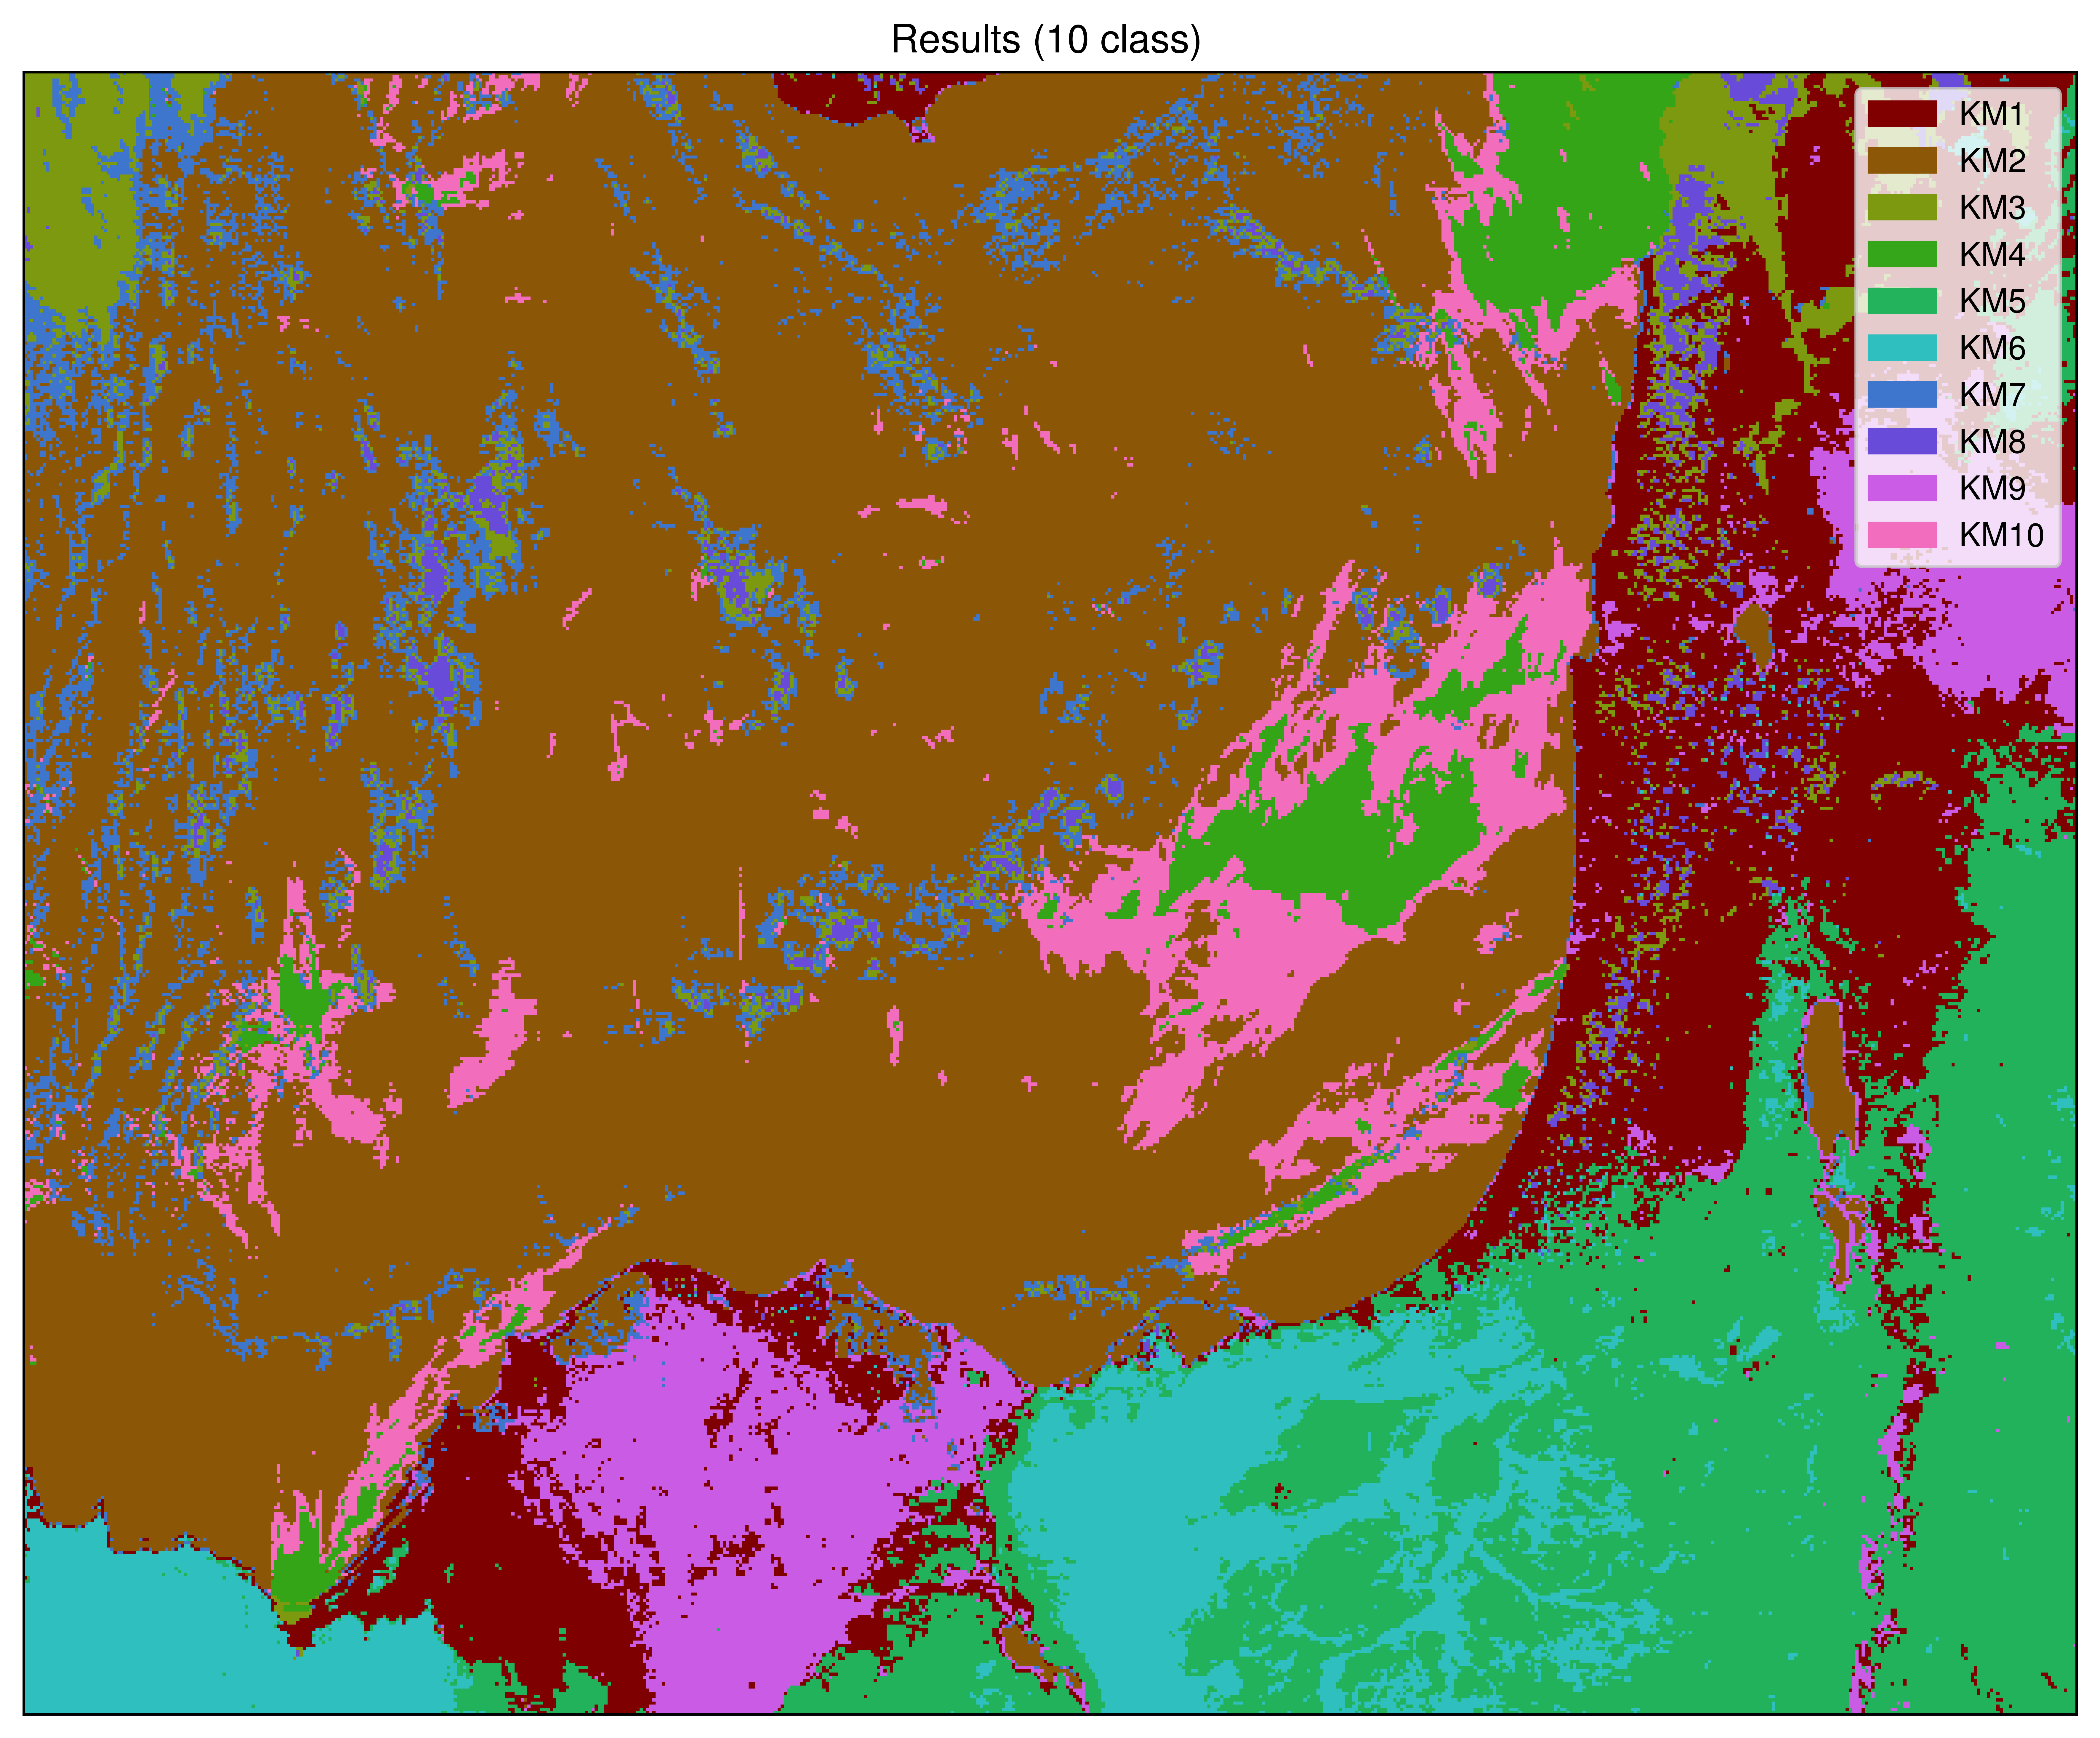
\includegraphics[width=.45\paperwidth]{figs/class/kmeans_batch9c10_10c.png}
            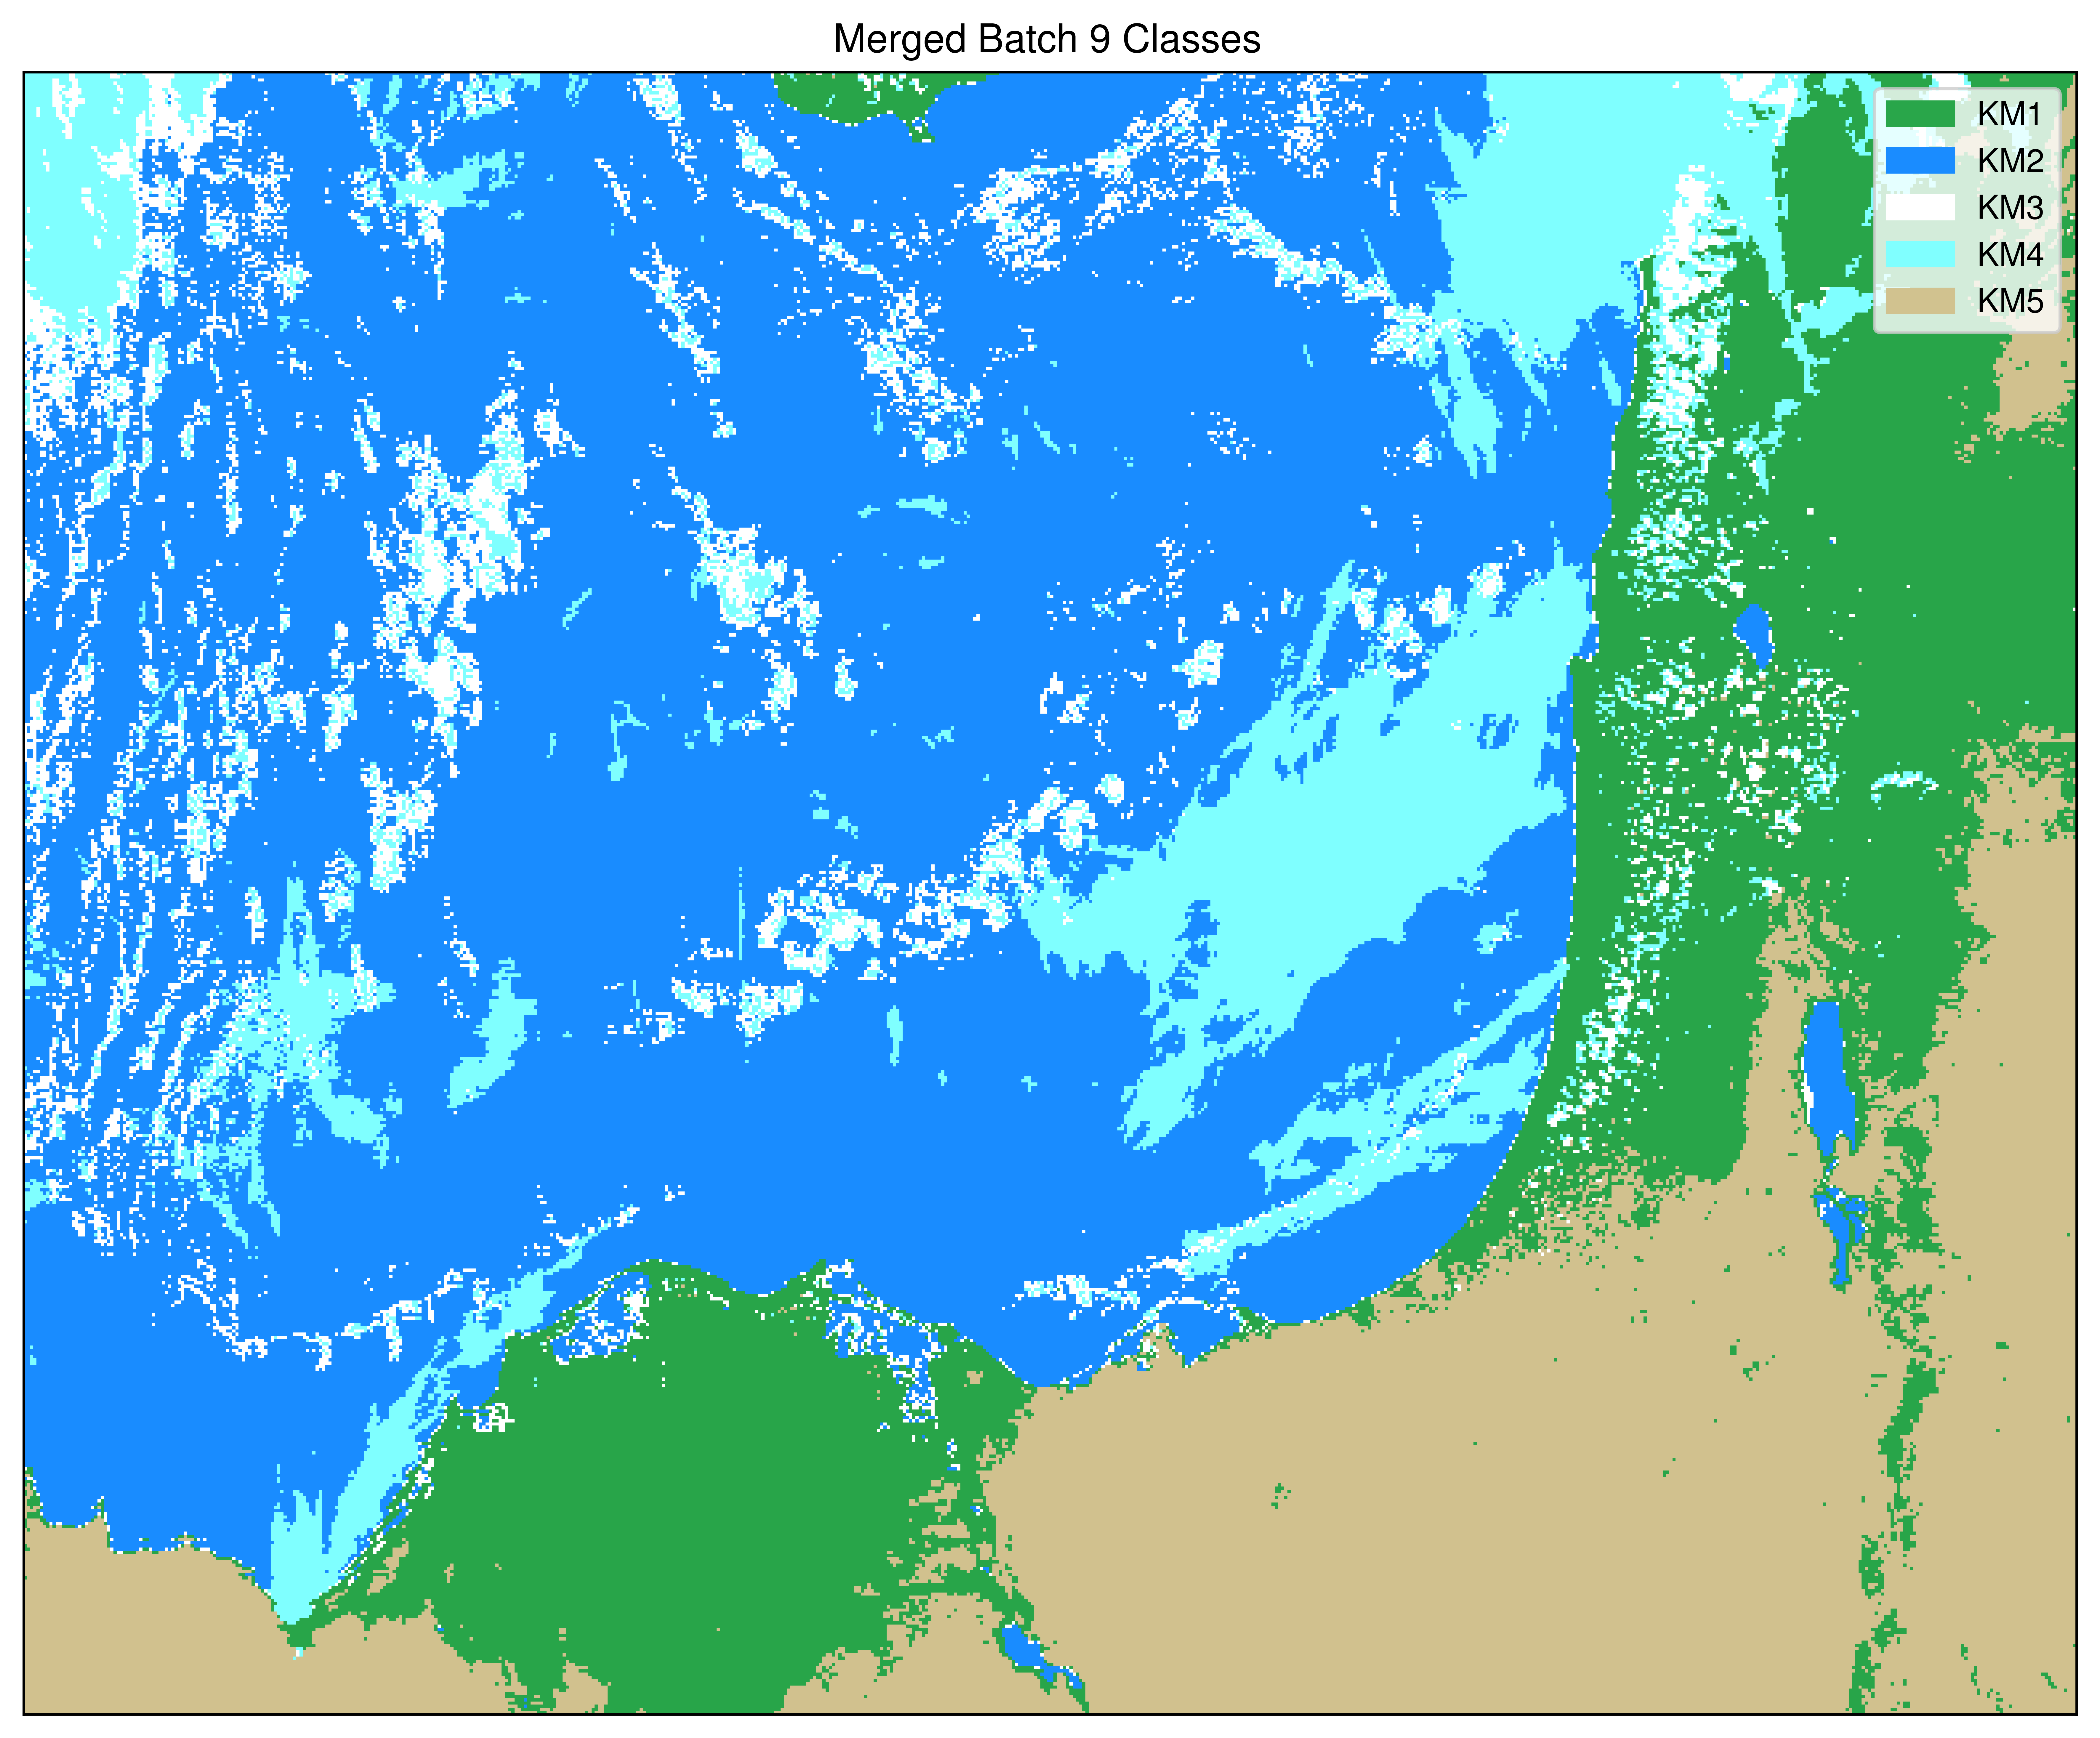
\includegraphics[width=.45\paperwidth]{figs/class/kmeans_merged2_5c.png}
        }
    \end{center}
    \caption{Final set of K-means results, which were trained on the 11 starred bands in Table \ref{band_table}. I determined that 10 classes was an appropriate number of categories to capture a variety of features without finding mean vectors that are too close together given the bands I selected. These 10 classes were subsequently manually merged to reflect the 5 surface classes I chose for analysis.}
    \label{km_results}
\end{figure}

\begin{figure}[h!]
    \centering
    \begin{tabular}{c|cccccc}
        & KM1 & KM2 & KM3 & KM4 & KM5 \\
        & \footnotesize{(vegetation)} & \footnotesize{(water)} & \footnotesize{(water cloud)} & \footnotesize{(ice cloud)}& \footnotesize{(arid)} \\
        \hline
        Pixel Count & 57,991 & 149,596 & 20,064 & 37,428 & 62,601 \\
        Area (km$^2$) & 71,817 & 277,355 & 42,338 & 58,480 & 78,696 \\
    \end{tabular}
    \caption{Area and quantity of K-means pixel classes.}
    \label{km_areas}
\end{figure}

\clearpage

\begin{figure}[h!]
    \centering

    \begin{center}
        \makebox[\textwidth]{
            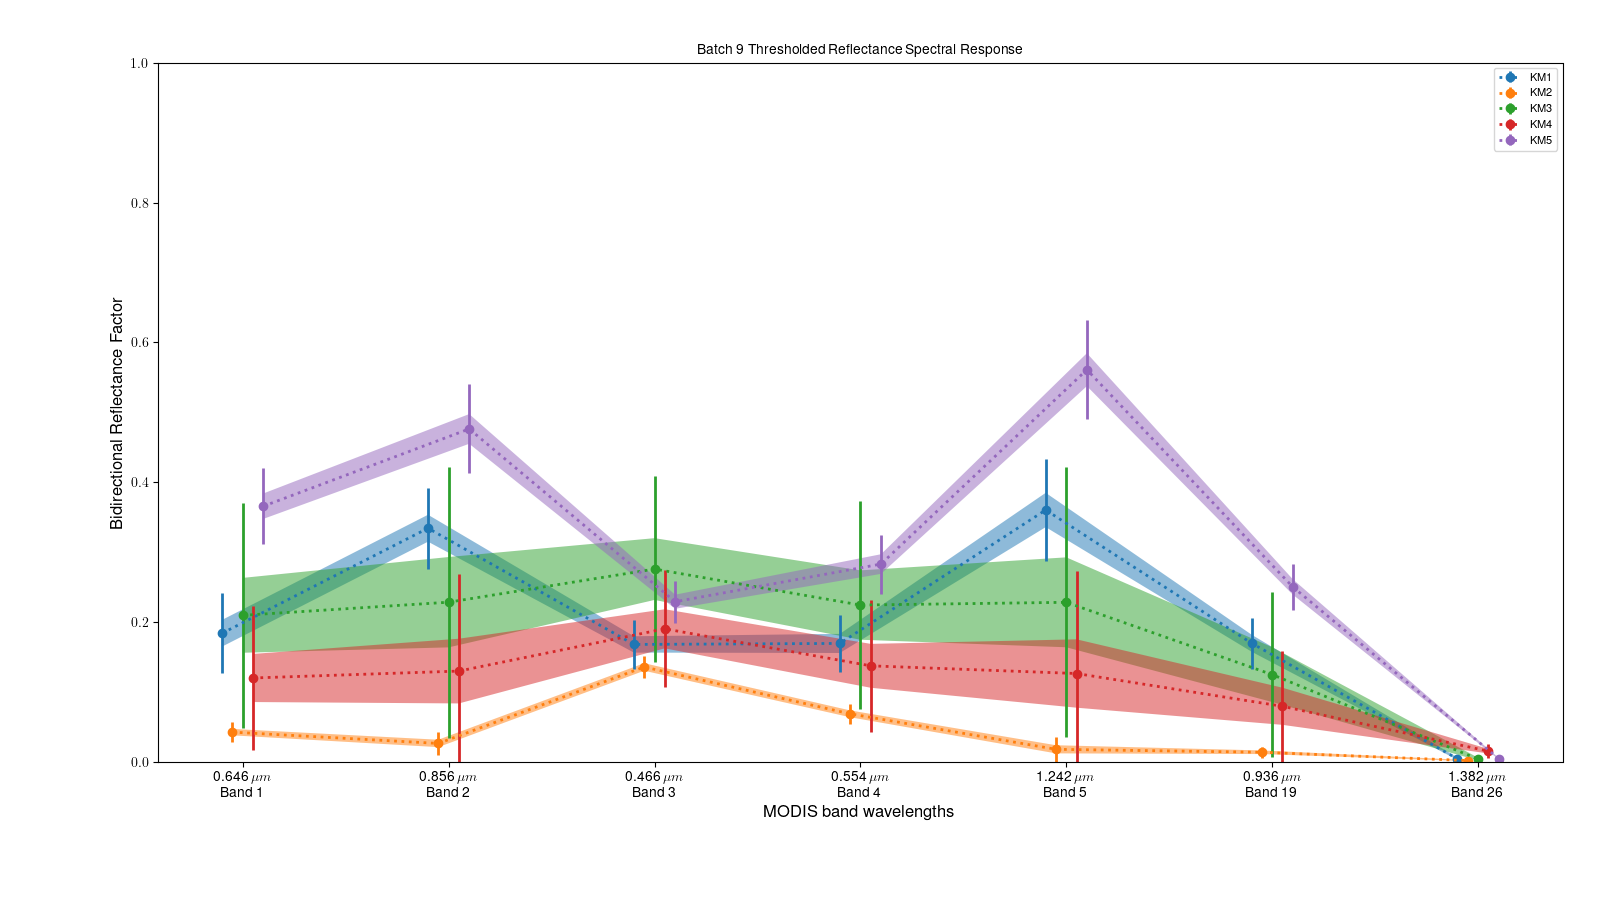
\includegraphics[width=.85\paperwidth]{figs/spectra/ref_km_b9.png}
        }
        \makebox[\textwidth]{
            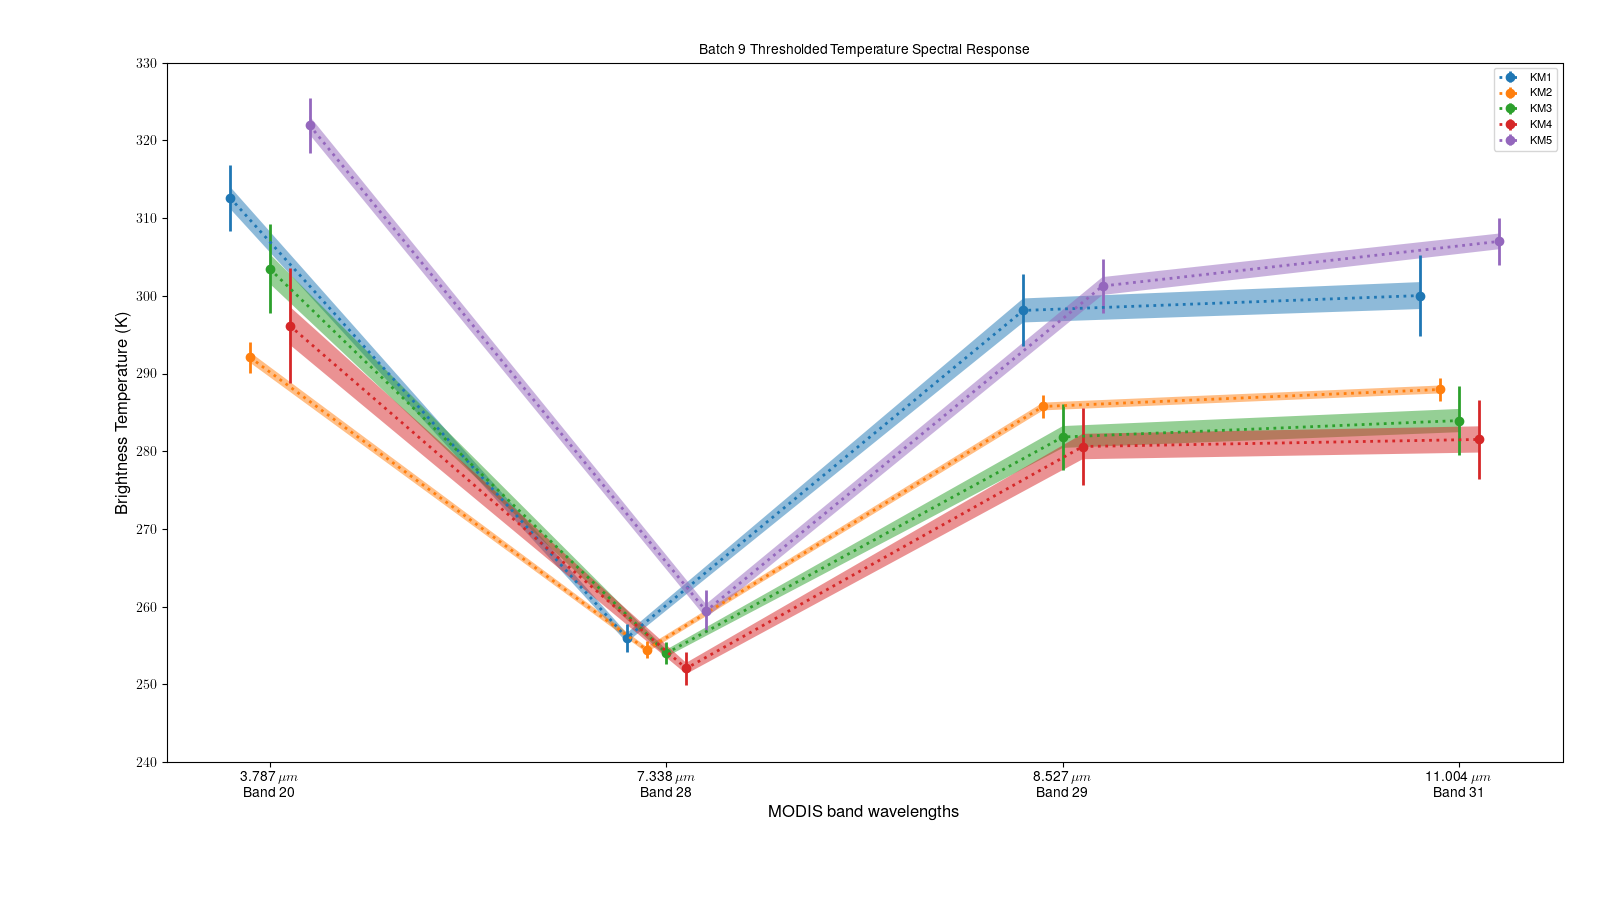
\includegraphics[width=.85\paperwidth]{figs/spectra/temp_km_b9.png}
        }
    \end{center}

    \caption{Mean spectral response of K-means classes for each of the bands used as classification inputs, with $1-\sigma$ error bars and $\frac{1}{3}-\sigma$ shaded regions. Top: reflectance bands, bottom: emissive bands.}
    \label{km_results}
\end{figure}

\clearpage


\begin{table}[h!]
\centering
\begin{tabular}{C|C|C|CCCCCCC}

\lambda & \mu & \sigma & \multicolumn{7}{c}{Reflectance Covariance $(\times10^{4})$} \\

\hline
    \multicolumn{10}{c}{KM1 (Vegetation)} \\
\hline
0.466 & 0.168 & 0.035 & 12.3 & 13.4 & 15.3 & 11.1 & 5.7 & 14.8 & 0.5 \\
0.554 & 0.170 & 0.041 & 13.4 & 16.8 & 22.0 & 15.7 & 9.4 & 22.0 & 0.7 \\
0.646 & 0.184 & 0.057 & 15.3 & 22.0 & 32.7 & 20.4 & 14.1 & 31.3 & 1.2 \\
0.856 & 0.334 & 0.058 & 11.1 & 15.7 & 20.4 & 33.3 & 17.6 & 39.2 & 0.7 \\
0.936 & 0.170 & 0.036 & 5.7 & 9.4 & 14.1 & 17.6 & 13.3 & 22.8 & 1.0 \\
1.242 & 0.361 & 0.074 & 14.8 & 22.0 & 31.3 & 39.2 & 22.8 & 54.1 & 1.3 \\
1.382 & 0.005 & 0.005 & 0.5 & 0.7 & 1.2 & 0.7 & 1.0 & 1.3 & 0.3 \\

\hline
    \multicolumn{10}{c}{KM2 (Water)} \\
\hline
0.466 & 0.043 & 0.014 & 1.9 & 2.1 & 1.8 & 1.9 & 2.3 & 1.0 & 0.0 \\
0.554 & 0.027 & 0.016 & 2.1 & 2.5 & 1.8 & 2.0 & 2.7 & 1.2 & 0.0 \\
0.646 & 0.136 & 0.016 & 1.8 & 1.8 & 2.6 & 1.9 & 1.9 & 0.8 & -0.1 \\
0.856 & 0.069 & 0.015 & 1.9 & 2.0 & 1.9 & 2.1 & 2.2 & 0.9 & 0.0 \\
0.936 & 0.018 & 0.018 & 2.3 & 2.7 & 1.9 & 2.2 & 3.1 & 1.3 & 0.0 \\
1.242 & 0.014 & 0.008 & 1.0 & 1.2 & 0.8 & 0.9 & 1.3 & 0.6 & 0.0 \\
1.382 & 0.002 & 0.002 & 0.0 & 0.0 & -0.1 & 0.0 & 0.0 & 0.0 & 0.1 \\

\hline
    \multicolumn{10}{c}{KM3 (Water Cloud)} \\
\hline
0.466 & 0.210 & 0.161 & 257.8 & 308.1 & 210.7 & 238.6 & 301.9 & 185.3 & 5.3 \\
0.554 & 0.229 & 0.194 & 308.1 & 375.5 & 249.0 & 284.6 & 370.1 & 226.1 & 6.7 \\
0.646 & 0.276 & 0.133 & 210.7 & 249.0 & 175.6 & 195.9 & 243.7 & 149.3 & 4.0 \\
0.856 & 0.225 & 0.149 & 238.6 & 284.6 & 195.9 & 221.2 & 278.7 & 171.0 & 4.8 \\
0.936 & 0.228 & 0.193 & 301.9 & 370.1 & 243.7 & 278.7 & 372.0 & 223.3 & 6.7 \\
1.242 & 0.125 & 0.118 & 185.3 & 226.1 & 149.3 & 171.0 & 223.3 & 138.1 & 4.5 \\
1.382 & 0.004 & 0.006 & 5.3 & 6.7 & 4.0 & 4.8 & 6.7 & 4.5 & 0.3 \\

\hline
    \multicolumn{10}{c}{KM4 (Ice Cloud)} \\
\hline
0.466 & 0.120 & 0.103 & 106.5 & 138.2 & 82.6 & 96.6 & 143.1 & 78.3 & -0.1 \\
0.554 & 0.130 & 0.139 & 138.2 & 192.6 & 101.1 & 123.8 & 201.5 & 109.2 & 0.7 \\
0.646 & 0.191 & 0.084 & 82.6 & 101.1 & 70.4 & 77.2 & 104.5 & 56.7 & -0.8 \\
0.856 & 0.138 & 0.094 & 96.6 & 123.8 & 77.2 & 88.6 & 128.0 & 69.9 & -0.3 \\
0.936 & 0.127 & 0.147 & 143.1 & 201.5 & 104.5 & 128.0 & 215.0 & 114.3 & 0.8 \\
1.242 & 0.080 & 0.080 & 78.3 & 109.2 & 56.7 & 69.9 & 114.3 & 63.4 & 1.2 \\
1.382 & 0.016 & 0.010 & -0.1 & 0.7 & -0.8 & -0.3 & 0.8 & 1.2 & 0.9 \\

\hline
    \multicolumn{10}{c}{KM5 (Arid)} \\
\hline
0.466 & 0.366 & 0.055 & 29.8 & 33.7 & 13.9 & 22.0 & 34.6 & 10.5 & -0.3 \\
0.554 & 0.476 & 0.064 & 33.7 & 40.6 & 15.9 & 24.9 & 42.0 & 11.5 & -0.5 \\
0.646 & 0.229 & 0.030 & 13.9 & 15.9 & 9.2 & 12.0 & 15.9 & 3.8 & -0.3 \\
0.856 & 0.283 & 0.042 & 22.0 & 24.9 & 12.0 & 17.8 & 25.1 & 7.5 & -0.3 \\
0.936 & 0.561 & 0.071 & 34.6 & 42.0 & 15.9 & 25.1 & 49.8 & 12.8 & -0.5 \\
1.242 & 0.251 & 0.033 & 10.5 & 11.5 & 3.8 & 7.5 & 12.8 & 10.9 & 0.4 \\
1.382 & 0.005 & 0.003 & -0.3 & -0.5 & -0.3 & -0.3 & -0.5 & 0.4 & 0.1 \\

\end{tabular}
\caption{Mean class values and standard devia for each reflectance band and covariance matrices for each surface type identified by K-means classification.}
\label{km_ref_stats}
\end{table}

\clearpage

\begin{table}[h!]
\centering
\begin{tabular}{C|C|C|CCCC}

\lambda & \mu & \sigma & \multicolumn{4}{c}{Brightness Temp. Covariance $(\times10^{2})$} \\

\hline
\multicolumn{7}{c}{KM1} \\
\hline
3.79 & 312.6 & 4.23 & 1793.4 & 395.7 & 1422.1 & 1661.1 \\
7.34 & 256.0 & 1.79 & 395.7 & 319.0 & 470.3 & 586.3 \\
8.53 & 298.1 & 4.63 & 1422.1 & 470.3 & 2146.3 & 2363.0 \\
11.00 & 300.0 & 5.20 & 1661.1 & 586.3 & 2363.0 & 2704.1 \\

\hline
\multicolumn{7}{c}{KM2} \\
\hline
3.79 & 292.1 & 2.01 & 404.0 & 60.5 & 94.8 & 83.7 \\
7.34 & 254.5 & 1.12 & 60.5 & 126.4 & 114.8 & 107.6 \\
8.53 & 285.8 & 1.51 & 94.8 & 114.8 & 228.1 & 223.0 \\
11.00 & 287.9 & 1.53 & 83.7 & 107.6 & 223.0 & 233.9 \\

\hline
\multicolumn{7}{c}{KM3} \\
\hline
3.79 & 303.5 & 5.72 & 3276.2 & 110.1 & -959.3 & -1048.7 \\
7.34 & 254.0 & 1.39 & 110.1 & 193.1 & 311.5 & 332.5 \\
8.53 & 281.8 & 4.22 & -959.3 & 311.5 & 1777.6 & 1873.9 \\
11.00 & 284.0 & 4.48 & -1048.7 & 332.5 & 1873.9 & 2009.4 \\

\hline
\multicolumn{7}{c}{KM4} \\
\hline
3.79 & 296.2 & 7.35 & 5405.7 & 478.3 & -1124.8 & -932.1 \\
7.34 & 252.1 & 2.17 & 478.3 & 469.9 & 459.4 & 596.8 \\
8.53 & 280.6 & 4.90 & -1124.8 & 459.4 & 2404.9 & 2440.2 \\
11.00 & 281.5 & 5.06 & -932.1 & 596.8 & 2440.2 & 2563.5 \\

\hline
\multicolumn{7}{c}{KM5} \\
\hline
3.79 & 322.0 & 3.55 & 1257.1 & 272.8 & -185.0 & 741.5 \\
7.34 & 259.4 & 2.66 & 272.8 & 709.5 & 412.8 & 470.0 \\
8.53 & 301.3 & 3.45 & -185.0 & 412.8 & 1192.0 & 460.9 \\
11.00 & 307.0 & 3.03 & 741.5 & 470.0 & 460.9 & 918.3 \\

\end{tabular}
\caption{Mean class values and standard devia for each emissive band and covariance matrices for each surface type identified by K-means classification.}
\label{km_temp_stats}
\end{table}


\begin{table}[h!]
\centering
\begin{tabular}{C|CCCCC|C}
& \textnormal{Ice Cloud} & \textnormal{Water Cloud} & \textnormal{Vegetation} & \textnormal{Water} & \textnormal{Arid} & \textnormal{Cons. Acc.} \\
\hline
\textnormal{KM1} & 766 & 0 & 35940 & 0 & 8023 & 0.804 \\
\textnormal{KM2} & 0 & 0 & 195 & 96348 & 79 & 0.997 \\
\textnormal{KM3} & 518 & 2213 & 326 & 0 & 5 & 0.723 \\
\textnormal{KM4} & 8736 & 12 & 0 & 382 & 0 & 0.957 \\
\textnormal{KM5} & 74 & 2 & 153 & 0 & 60815 & 0.996 \\

\hline
\textnormal{Prod. Acc.} & 0.865 & 0.994 & 0.982 & 0.996 & 0.882\\
\end{tabular}
\caption{Confusion matrix comparing my threshold-derived surface classes to the K-means results.}
\label{confusion_km-thresh}
\end{table}

\clearpage

\section{Samples from thresholded classes}


\begin{figure}[h!]
    \centering

    \begin{center}
        \makebox[\textwidth]{
            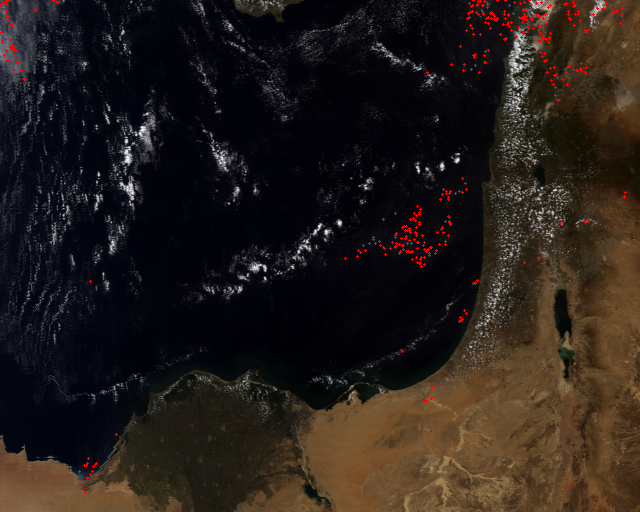
\includegraphics[width=.3\paperwidth]{figs/masks/cmask_samples_thresh_ice_cloud_TC.png}
            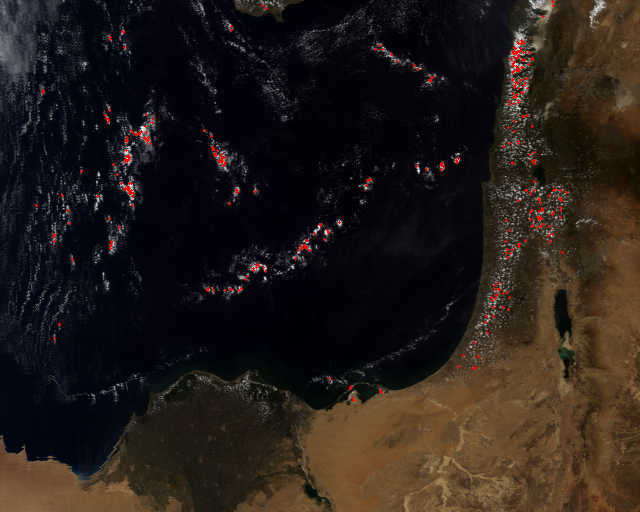
\includegraphics[width=.3\paperwidth]{figs/masks/cmask_samples_thresh_water_cloud_TC.png}
        }

        \vspace{.2em}

        \makebox[\textwidth]{
            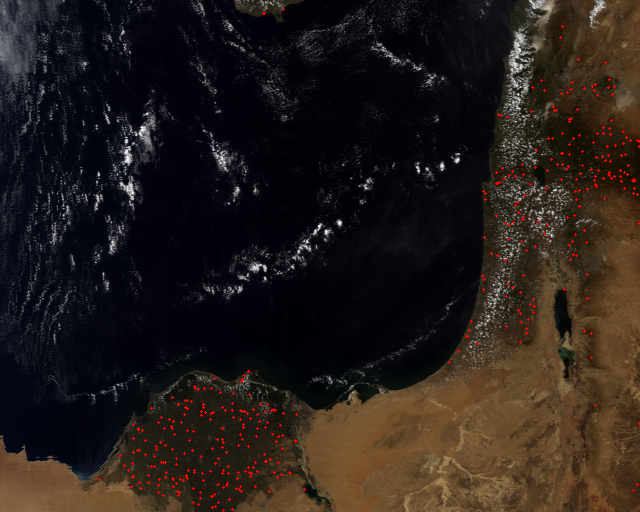
\includegraphics[width=.3\paperwidth]{figs/masks/cmask_samples_thresh_vegetation_TC.png}
            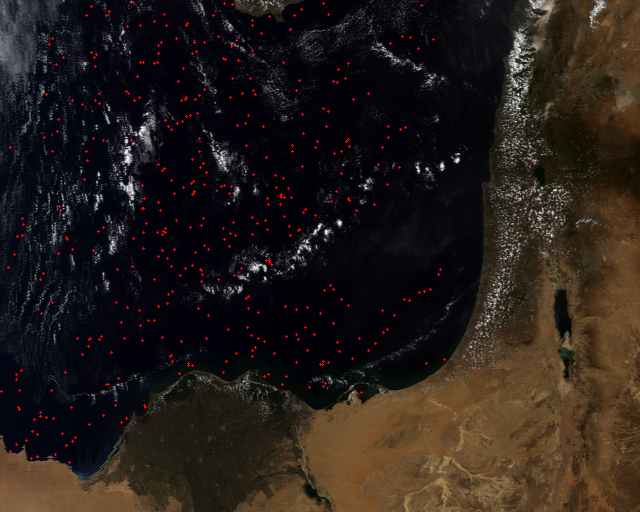
\includegraphics[width=.3\paperwidth]{figs/masks/cmask_samples_thresh_water_TC.png}
            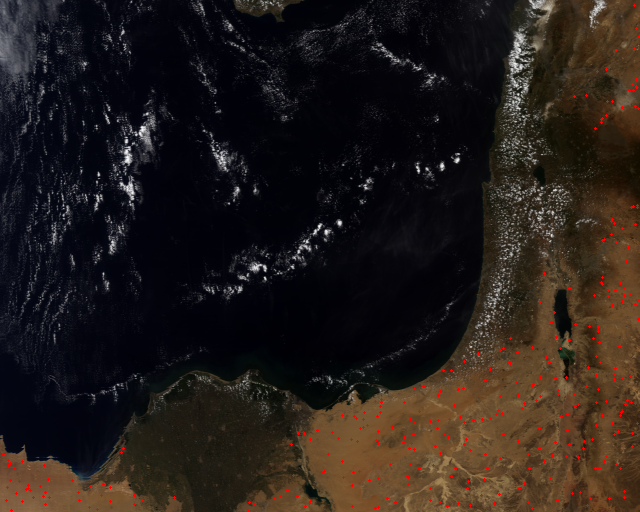
\includegraphics[width=.3\paperwidth]{figs/masks/cmask_samples_thresh_arid_TC.png}
        }
    \end{center}

    \caption{Pixels chosen from subsets of each threshold class mask. Top: ice cloud and water cloud samples. Bottom: vegetation, water, and arid land samples.}
    \label{thresh_samples}
\end{figure}

\begin{figure}[h!]
    \centering
    \begin{tabular}{c|cccccc}
    & Ice Cloud & Water Cloud & Vegetation & Water & Arid \\
    \hline
    Pixel Count & 393 & 369 & 397 & 399 & 399\\
    Area (km$^2$) & 560 & 519 & 532 & 742 & 518\\
    \end{tabular}
    \caption{Area and quantity of samples chosen from thresholded pixel classes. 400 random pixels were selected for each class, and repeated indeces were dropped. Although the same number of samples were selected for water and arid surfaces, the surface area of the water samples is much higher due to additional panoramic distortion on the left side of the image.}
    \label{sample_thresh_areas}
\end{figure}


\clearpage

\begin{figure}[h!]
    \centering

    \begin{center}
        \makebox[\textwidth]{
            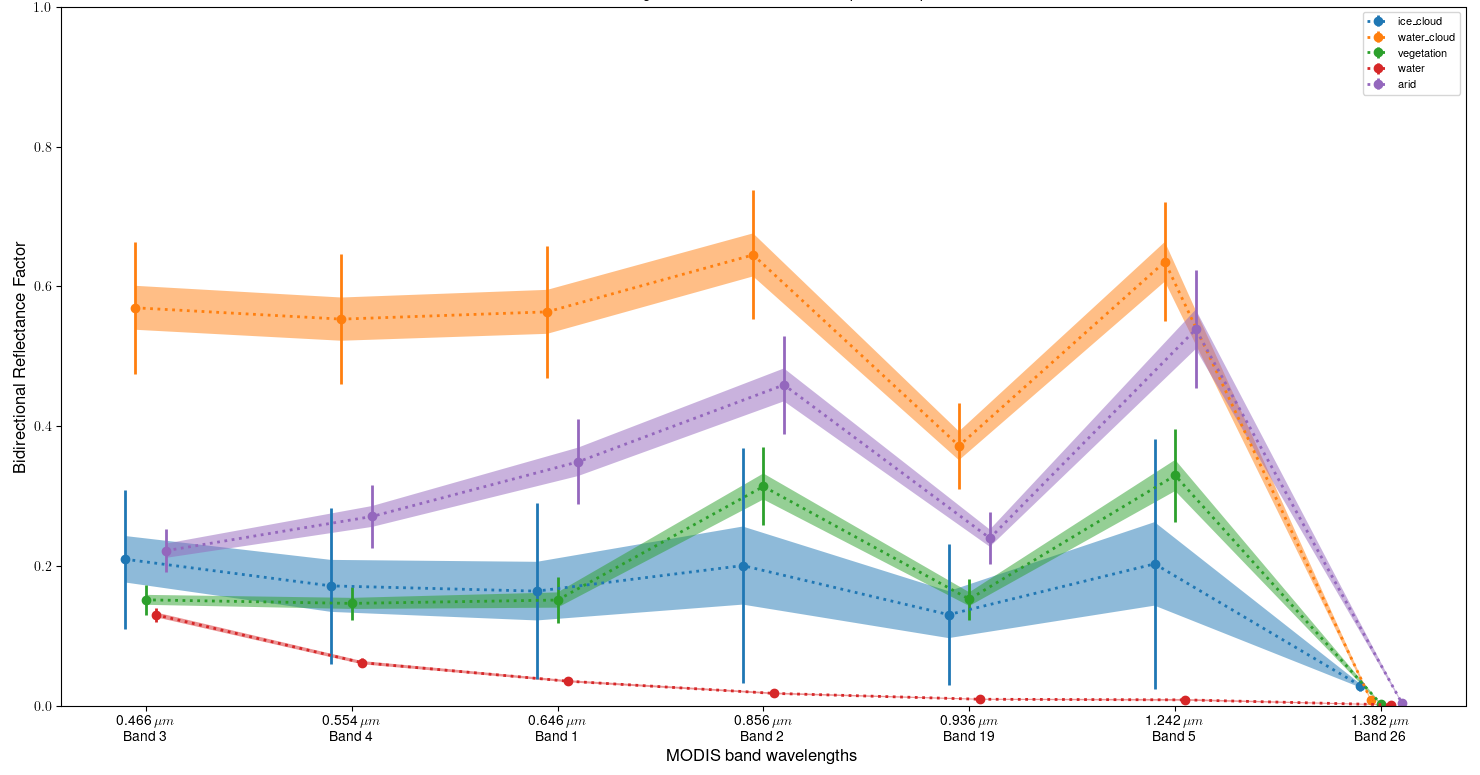
\includegraphics[width=.85\paperwidth]{figs/spectra/ref_samples_thresh_b9_cropped.png}
        }
        \makebox[\textwidth]{
            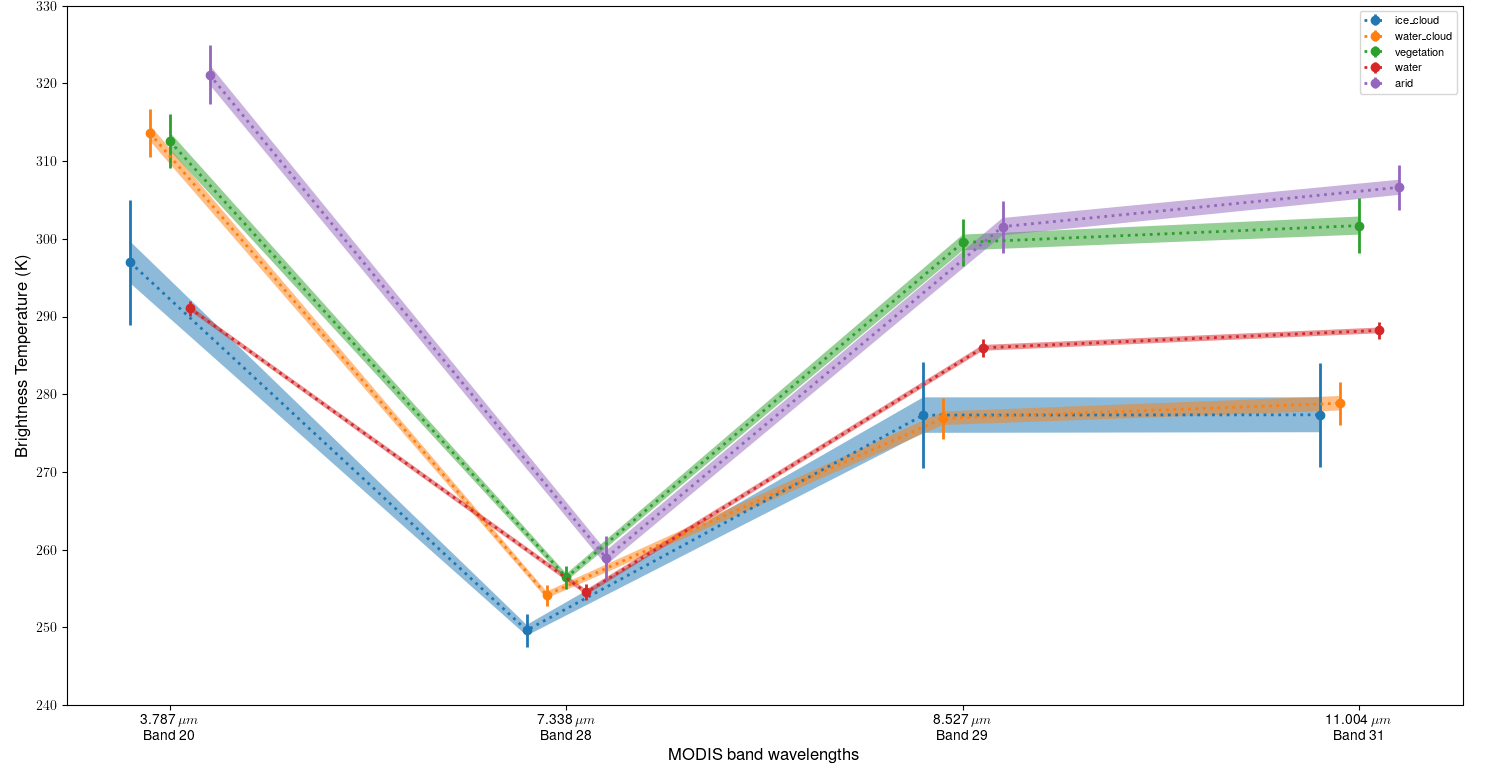
\includegraphics[width=.85\paperwidth]{figs/spectra/temp_samples_thresh_b9_cropped.png}
        }
    \end{center}

    \caption{}
    \label{samples_thresh_spectra}
\end{figure}


\clearpage

\clearpage

\begin{figure}[h!]
\centering
\begin{tabular}{C|C|C|CCCCCCC}

\lambda & \mu & \sigma & \multicolumn{7}{c}{Reflectance Covariance $(\times10^{4})$} \\

\hline
\multicolumn{10}{c}{Ice Cloud} \\
\hline
0.466 & 0.210 & 0.100 & 99.5 & 106.9 & 113.7 & 126.1 & 79.8 & 122.4 & 0.0 \\
0.554 & 0.172 & 0.112 & 106.9 & 124.6 & 138.7 & 168.7 & 103.6 & 168.5 & 0.3 \\
0.646 & 0.164 & 0.126 & 113.7 & 138.7 & 158.5 & 199.1 & 120.8 & 202.2 & 0.4 \\
0.856 & 0.201 & 0.167 & 126.1 & 168.7 & 199.1 & 281.1 & 167.1 & 295.0 & 1.4 \\
0.936 & 0.131 & 0.101 & 79.8 & 103.6 & 120.8 & 167.1 & 101.4 & 174.4 & 1.1 \\
1.242 & 0.203 & 0.179 & 122.4 & 168.5 & 202.2 & 295.0 & 174.4 & 321.5 & 1.5 \\
1.382 & 0.029 & 0.008 & 0.0 & 0.3 & 0.4 & 1.4 & 1.1 & 1.5 & 0.6 \\

\hline
\multicolumn{10}{c}{Water Cloud} \\
\hline
0.466 & 0.564 & 0.094 & 89.2 & 82.8 & 87.2 & 87.3 & 66.0 & 47.4 & -0.4 \\
0.554 & 0.645 & 0.092 & 82.8 & 85.4 & 78.3 & 80.7 & 72.0 & 52.2 & 0.5 \\
0.646 & 0.570 & 0.094 & 87.2 & 78.3 & 89.1 & 86.8 & 61.0 & 42.3 & -1.0 \\
0.856 & 0.553 & 0.093 & 87.3 & 80.7 & 86.8 & 86.2 & 63.9 & 45.7 & -0.5 \\
0.936 & 0.635 & 0.085 & 66.0 & 72.0 & 61.0 & 63.9 & 72.6 & 46.0 & 0.9 \\
1.242 & 0.372 & 0.062 & 47.4 & 52.2 & 42.3 & 45.7 & 46.0 & 38.3 & 1.4 \\
1.382 & 0.009 & 0.006 & -0.4 & 0.5 & -1.0 & -0.5 & 0.9 & 1.4 & 0.3 \\

\hline
\multicolumn{10}{c}{Vegetation} \\
\hline
0.466 & 0.152 & 0.033 & 10.8 & 8.4 & 4.8 & 7.0 & 15.1 & 5.4 & 0.3 \\
0.554 & 0.314 & 0.056 & 8.4 & 31.2 & 4.9 & 7.7 & 33.6 & 13.5 & 0.0 \\
0.646 & 0.152 & 0.021 & 4.8 & 4.9 & 4.6 & 4.6 & 7.4 & 0.9 & -0.0 \\
0.856 & 0.147 & 0.024 & 7.0 & 7.7 & 4.6 & 5.7 & 11.5 & 3.3 & 0.1 \\
0.936 & 0.330 & 0.067 & 15.1 & 33.6 & 7.4 & 11.5 & 44.7 & 16.2 & 0.3 \\
1.242 & 0.153 & 0.030 & 5.4 & 13.5 & 0.9 & 3.3 & 16.2 & 8.7 & 0.3 \\
1.382 & 0.003 & 0.003 & 0.3 & 0.0 & -0.0 & 0.1 & 0.3 & 0.3 & 0.1 \\

\hline
\multicolumn{10}{c}{Water} \\
\hline
0.466 & 0.036 & 0.004 & 0.2 & 0.1 & 0.3 & 0.3 & 0.1 & 0.1 & 0.0 \\
0.554 & 0.018 & 0.004 & 0.1 & 0.1 & 0.2 & 0.1 & 0.1 & 0.1 & 0.0 \\
0.646 & 0.131 & 0.010 & 0.3 & 0.2 & 1.1 & 0.5 & 0.1 & 0.0 & -0.0 \\
0.856 & 0.062 & 0.007 & 0.3 & 0.1 & 0.5 & 0.5 & 0.1 & 0.1 & 0.0 \\
0.936 & 0.009 & 0.004 & 0.1 & 0.1 & 0.1 & 0.1 & 0.1 & 0.1 & 0.0 \\
1.242 & 0.010 & 0.002 & 0.1 & 0.1 & 0.0 & 0.1 & 0.1 & 0.0 & 0.0 \\
1.382 & 0.002 & 0.002 & 0.0 & 0.0 & -0.0 & 0.0 & 0.0 & 0.0 & 0.0 \\

\hline
\multicolumn{10}{c}{Arid} \\
\hline
0.466 & 0.349 & 0.061 & 37.3 & 41.6 & 16.5 & 26.5 & 47.5 & 14.6 & -0.4 \\
0.554 & 0.459 & 0.071 & 41.6 & 49.9 & 18.5 & 29.6 & 56.9 & 16.4 & -0.6 \\
0.646 & 0.222 & 0.031 & 16.5 & 18.5 & 9.4 & 13.1 & 20.8 & 4.6 & -0.3 \\
0.856 & 0.271 & 0.045 & 26.5 & 29.6 & 13.1 & 20.1 & 33.4 & 9.7 & -0.3 \\
0.936 & 0.539 & 0.085 & 47.5 & 56.9 & 20.8 & 33.4 & 71.6 & 20.1 & -0.6 \\
1.242 & 0.240 & 0.037 & 14.6 & 16.4 & 4.6 & 9.7 & 20.1 & 13.7 & 0.4 \\
1.382 & 0.005 & 0.003 & -0.4 & -0.6 & -0.3 & -0.3 & -0.6 & 0.4 & 0.1 \\

\end{tabular}
\caption{Mean values and standard devia of reflectance pixels sampled from thresholded classes. Includes mean reflectance and standard deviation for each band and covariance matrices for the 5 surface types I identified.}
\label{samples_thresh_ref_stats}
\end{figure}

\clearpage

\begin{figure}[h!]
\centering
\begin{tabular}{C|C|C|CCCC}

\lambda & \mu & \sigma & \multicolumn{4}{c}{Brightness Temp. Covariance $(\times10^{2})$} \\

\hline
\multicolumn{7}{c}{Ice Cloud} \\
\hline
3.79 & 297.0 & 8.04 & 6484.6 & 688.3 & 18.0 & 410.4 \\
7.34 & 249.6 & 2.09 & 688.3 & 438.8 & 181.6 & 358.7 \\
8.53 & 277.3 & 6.86 & 18.0 & 181.6 & 4712.9 & 4547.5 \\
11.00 & 277.4 & 6.72 & 410.4 & 358.7 & 4547.5 & 4533.0 \\

\hline
\multicolumn{7}{c}{Water Cloud} \\
\hline
3.79 & 313.6 & 3.07 & 942.3 & 216.7 & 341.8 & 380.8 \\
7.34 & 254.2 & 1.35 & 216.7 & 183.3 & 242.5 & 280.3 \\
8.53 & 276.9 & 2.62 & 341.8 & 242.5 & 687.8 & 714.4 \\
11.00 & 278.8 & 2.79 & 380.8 & 280.3 & 714.4 & 781.0 \\

\hline
\multicolumn{7}{c}{Vegetation} \\
\hline
3.79 & 312.6 & 3.47 & 1210.5 & 273.0 & 844.8 & 1020.5 \\
7.34 & 256.4 & 1.44 & 273.0 & 209.3 & 253.8 & 336.3 \\
8.53 & 299.5 & 3.04 & 844.8 & 253.8 & 925.8 & 1022.5 \\
11.00 & 301.7 & 3.50 & 1020.5 & 336.3 & 1022.5 & 1226.4 \\

\hline
\multicolumn{7}{c}{Water} \\
\hline
3.79 & 291.1 & 0.97 & 94.3 & 60.7 & 87.6 & 77.9 \\
7.34 & 254.5 & 1.05 & 60.7 & 110.1 & 84.9 & 77.8 \\
8.53 & 286.0 & 1.12 & 87.6 & 84.9 & 126.2 & 118.8 \\
11.00 & 288.2 & 1.11 & 77.9 & 77.8 & 118.8 & 123.0 \\

\hline
\multicolumn{7}{c}{Arid} \\
\hline
3.79 & 321.1 & 3.80 & 1450.6 & 389.8 & -108.0 & 836.4 \\
7.34 & 258.9 & 2.81 & 389.8 & 792.3 & 366.1 & 493.1 \\
8.53 & 301.6 & 3.35 & -108.0 & 366.1 & 1123.1 & 424.3 \\
11.00 & 306.6 & 2.93 & 836.4 & 493.1 & 424.3 & 859.3 \\

\end{tabular}
\caption{Mean values and standard devia of brightness temperature pixels sampled from thresholded classes. Includes mean brightness temperature in Kelvin and standard deviation for each band and covariance matrices for the 5 surface types I identified.}
\label{samples_thresh_temp_stats}
\end{figure}

\clearpage
\section{Maximum-likelihood classification with threshold samples}

\begin{figure}[h!]
    \centering

    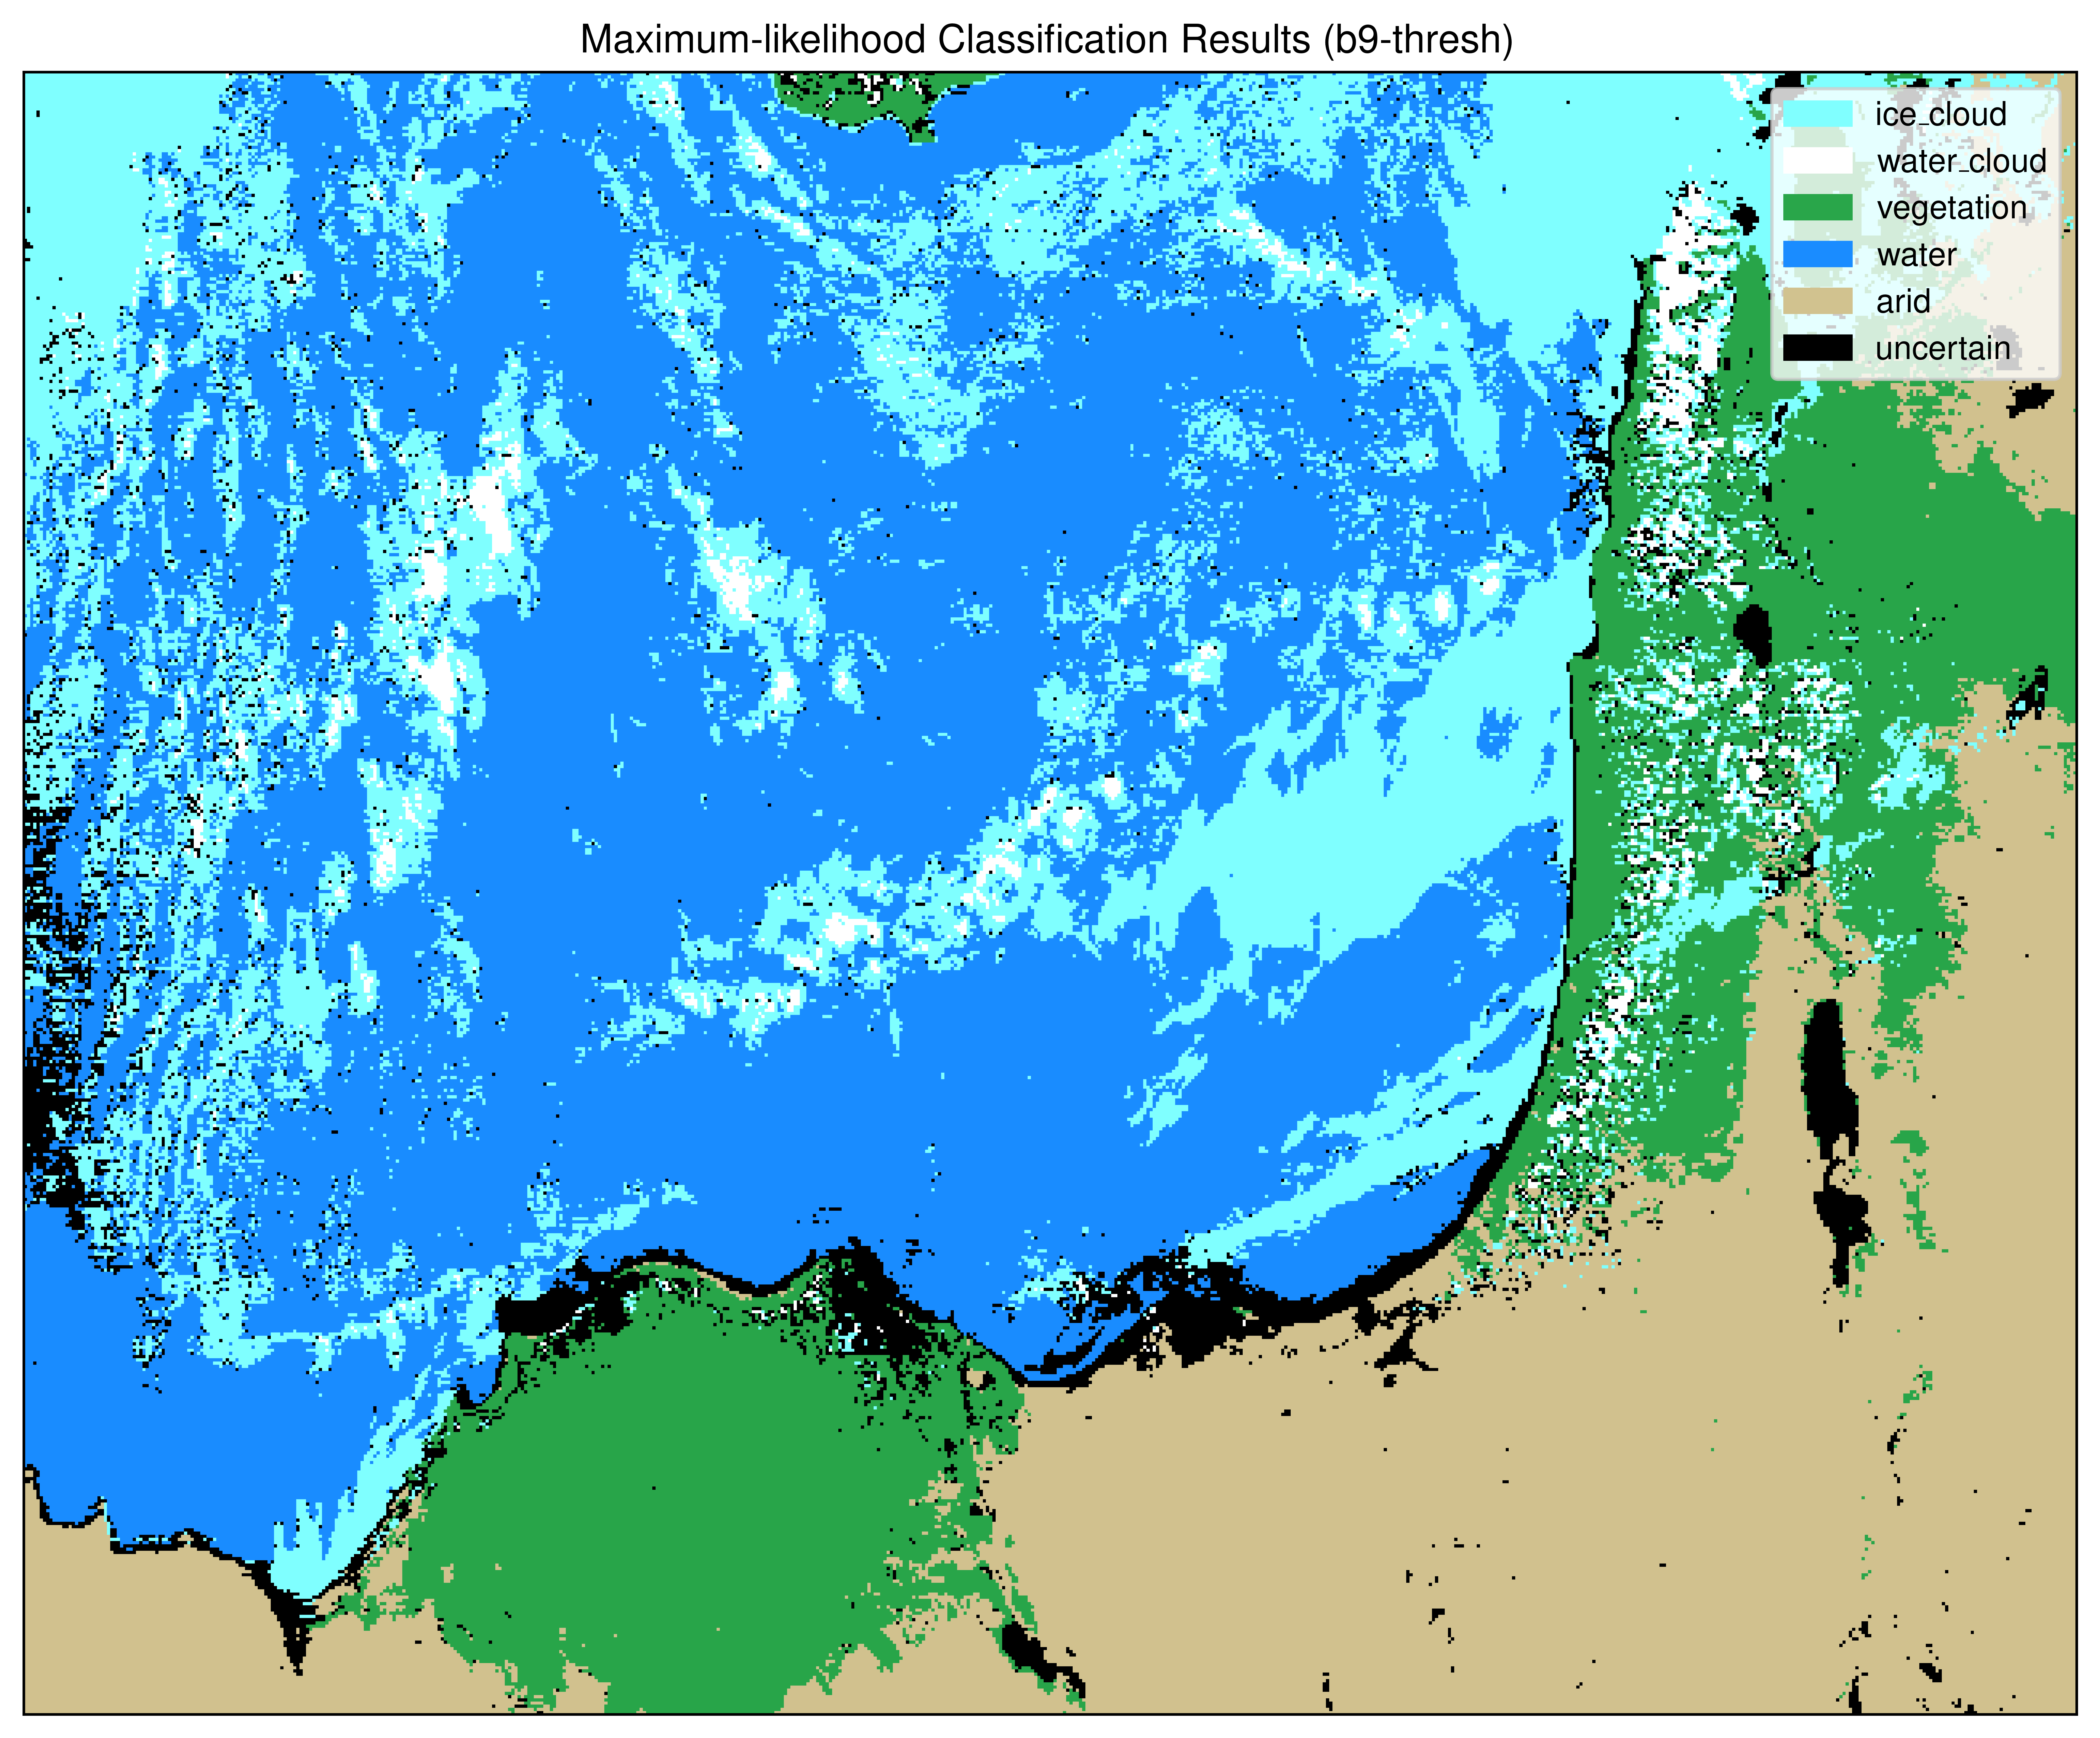
\includegraphics[width=.85\textwidth]{figs/class/mlc_b9-thresh_6c.png}

    \caption{Results from maximum-likelihood classification using threshold samples.  Pixels with a confidence less than $5\%$ are added to the ``uncertain'' class. }
    \label{mlc_thresh_results}
\end{figure}

\begin{figure}[h!]
    \centering
    \begin{tabular}{c|ccccccc}
    & Ice Cloud & Water Cloud & Vegetation & Water & Arid & Uncertain\\
    \hline
    Pixel Count & 69620 & 5799 & 43344 & 125432 & 68670 & 14815\\
    Area (km$^2$) & 124604 & 8654 & 55828 & 226847 & 85326 & 27429\\
    \end{tabular}
    \caption{Area and quantity of pixel classes identified with maximum-likelihood classification using samples chosen from thresholded classes.}
    \label{mlc_thresh_areas}
\end{figure}

\clearpage

\begin{figure}[h!]
    \centering

    \begin{center}
        \makebox[\textwidth]{
            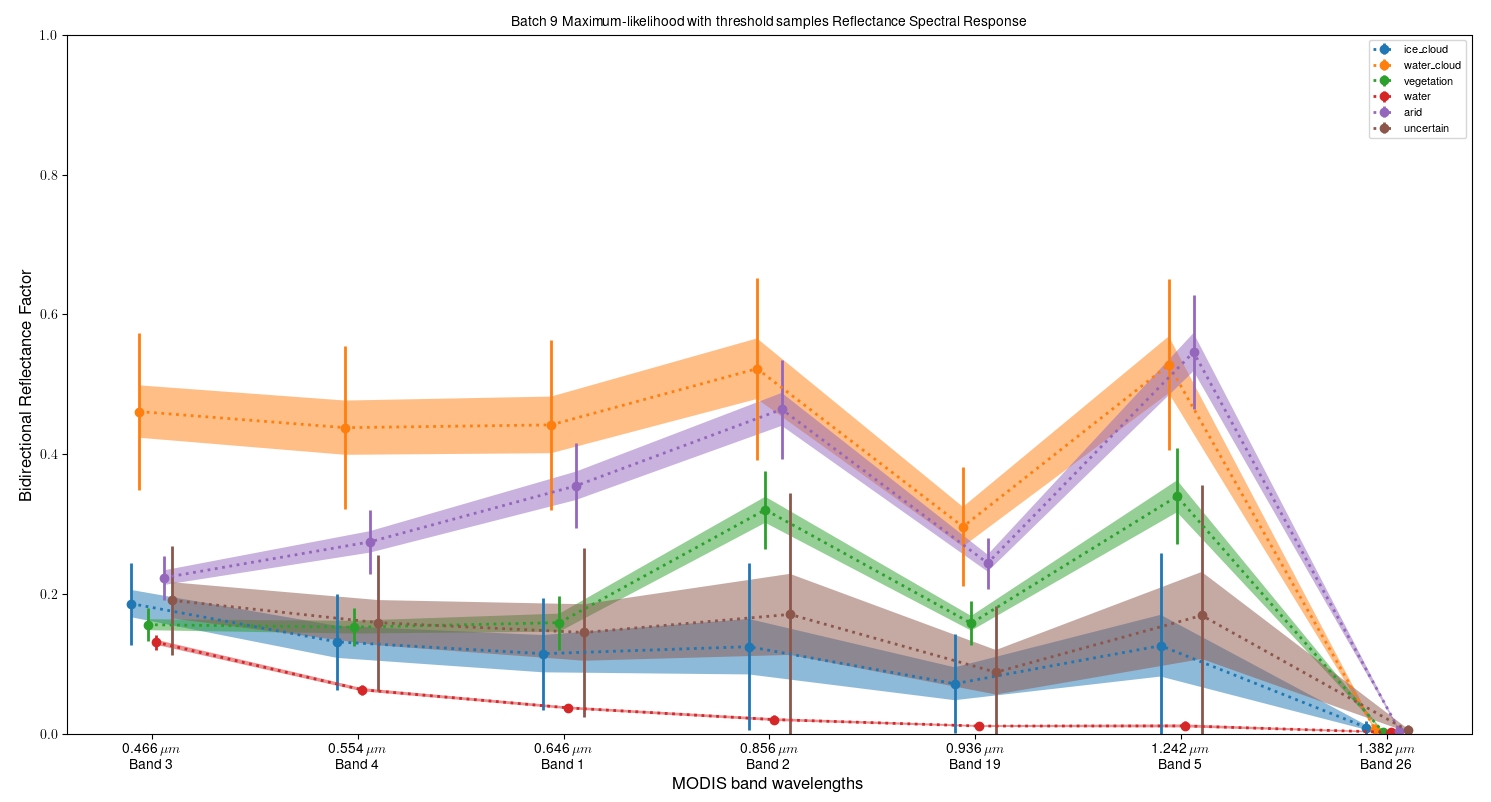
\includegraphics[width=.85\paperwidth]{figs/spectra/ref_mlc_thresh_b9_cropped.png}
        }
        \makebox[\textwidth]{
            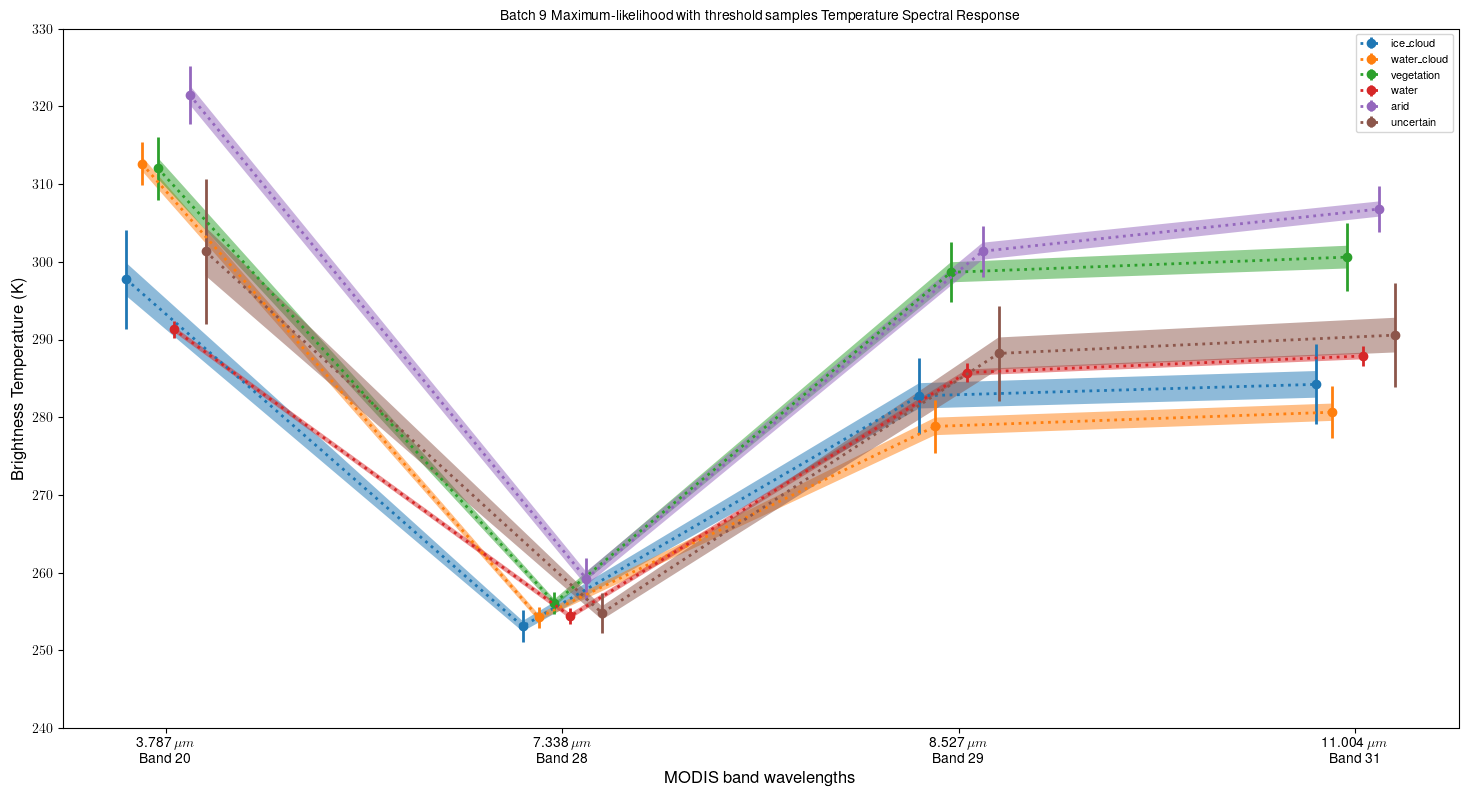
\includegraphics[width=.85\paperwidth]{figs/spectra/temp_mlc_thresh_b9_cropped.png}
        }
    \end{center}

    \caption{}
    \label{mlc_thresh_spectra}
\end{figure}


\clearpage

\begin{figure}[h!]
\centering
\begin{tabular}{C|C|C|CCCCCCC}

\lambda & \mu & \sigma & \multicolumn{7}{c}{Reflectance Covariance $(\times10^{4})$} \\

\hline
\multicolumn{10}{c}{Ice Cloud} \\
\hline
0.466 & 0.187 & 0.059 & 34.3 & 37.7 & 40.7 & 50.9 & 29.4 & 54.3 & 0.3 \\
0.554 & 0.132 & 0.069 & 37.7 & 47.3 & 54.2 & 75.0 & 43.8 & 81.4 & 1.2 \\
0.646 & 0.115 & 0.080 & 40.7 & 54.2 & 63.9 & 91.2 & 53.5 & 100.0 & 1.8 \\
0.856 & 0.125 & 0.119 & 50.9 & 75.0 & 91.2 & 141.8 & 82.9 & 156.7 & 3.3 \\
0.936 & 0.072 & 0.070 & 29.4 & 43.8 & 53.5 & 82.9 & 49.7 & 91.5 & 2.7 \\
1.242 & 0.126 & 0.132 & 54.3 & 81.4 & 100.0 & 156.7 & 91.5 & 175.2 & 3.5 \\
1.382 & 0.009 & 0.010 & 0.3 & 1.2 & 1.8 & 3.3 & 2.7 & 3.5 & 1.0 \\

\hline
\multicolumn{10}{c}{Water Cloud} \\
\hline
0.466 & 0.442 & 0.121 & 147.5 & 149.5 & 134.3 & 141.1 & 131.9 & 91.8 & 1.8 \\
0.554 & 0.522 & 0.130 & 149.5 & 168.8 & 129.2 & 141.6 & 154.0 & 107.3 & 3.3 \\
0.646 & 0.461 & 0.112 & 134.3 & 129.2 & 126.4 & 129.6 & 110.9 & 77.1 & 0.8 \\
0.856 & 0.438 & 0.116 & 141.1 & 141.6 & 129.6 & 135.4 & 123.9 & 86.4 & 1.5 \\
0.936 & 0.528 & 0.122 & 131.9 & 154.0 & 110.9 & 123.9 & 148.6 & 99.8 & 3.6 \\
1.242 & 0.297 & 0.085 & 91.8 & 107.3 & 77.1 & 86.4 & 99.8 & 72.4 & 3.0 \\
1.382 & 0.008 & 0.006 & 1.8 & 3.3 & 0.8 & 1.5 & 3.6 & 3.0 & 0.4 \\

\hline
\multicolumn{10}{c}{Vegetation} \\
\hline
0.466 & 0.159 & 0.039 & 15.0 & 11.3 & 6.7 & 9.9 & 18.8 & 6.9 & 0.5 \\
0.554 & 0.321 & 0.056 & 11.3 & 31.2 & 5.8 & 9.2 & 35.3 & 14.6 & 0.2 \\
0.646 & 0.156 & 0.024 & 6.7 & 5.8 & 5.6 & 5.9 & 8.6 & 1.6 & 0.1 \\
0.856 & 0.153 & 0.027 & 9.9 & 9.2 & 5.9 & 7.6 & 13.6 & 4.4 & 0.2 \\
0.936 & 0.340 & 0.069 & 18.8 & 35.3 & 8.6 & 13.6 & 46.9 & 18.2 & 0.6 \\
1.242 & 0.158 & 0.032 & 6.9 & 14.6 & 1.6 & 4.4 & 18.2 & 10.0 & 0.5 \\
1.382 & 0.003 & 0.004 & 0.5 & 0.2 & 0.1 & 0.2 & 0.6 & 0.5 & 0.1 \\

\hline
\multicolumn{10}{c}{Water} \\
\hline
0.466 & 0.038 & 0.006 & 0.3 & 0.3 & 0.4 & 0.4 & 0.3 & 0.2 & 0.0 \\
0.554 & 0.021 & 0.006 & 0.3 & 0.3 & 0.3 & 0.3 & 0.4 & 0.2 & 0.1 \\
0.646 & 0.131 & 0.011 & 0.4 & 0.3 & 1.2 & 0.6 & 0.2 & 0.1 & -0.0 \\
0.856 & 0.064 & 0.007 & 0.4 & 0.3 & 0.6 & 0.5 & 0.3 & 0.1 & 0.0 \\
0.936 & 0.012 & 0.006 & 0.3 & 0.4 & 0.2 & 0.3 & 0.4 & 0.2 & 0.1 \\
1.242 & 0.012 & 0.004 & 0.2 & 0.2 & 0.1 & 0.1 & 0.2 & 0.1 & 0.1 \\
1.382 & 0.003 & 0.003 & 0.0 & 0.1 & -0.0 & 0.0 & 0.1 & 0.1 & 0.1 \\

\hline
\multicolumn{10}{c}{Arid} \\
\hline
0.466 & 0.355 & 0.061 & 37.1 & 41.9 & 17.0 & 27.2 & 45.9 & 15.0 & -0.4 \\
0.554 & 0.464 & 0.071 & 41.9 & 49.8 & 19.2 & 30.6 & 54.8 & 16.8 & -0.5 \\
0.646 & 0.224 & 0.031 & 17.0 & 19.2 & 9.8 & 13.9 & 20.8 & 5.4 & -0.3 \\
0.856 & 0.275 & 0.046 & 27.2 & 30.6 & 13.9 & 21.2 & 33.3 & 10.5 & -0.4 \\
0.936 & 0.546 & 0.082 & 45.9 & 54.8 & 20.8 & 33.3 & 66.9 & 19.8 & -0.5 \\
1.242 & 0.245 & 0.036 & 15.0 & 16.8 & 5.4 & 10.5 & 19.8 & 13.3 & 0.3 \\
1.382 & 0.005 & 0.003 & -0.4 & -0.5 & -0.3 & -0.4 & -0.5 & 0.3 & 0.1 \\

\end{tabular}
\caption{Mean reflectance values and standard devia of each reflectance band, for each class identified by maximum-likelihood classification using pixel samples selected from band thresholds.}
\label{mlc_thresh_ref_stats}
\end{figure}

\clearpage

\begin{figure}[h!]
\centering
\begin{tabular}{C|C|C|CCCC}

\lambda & \mu & \sigma & \multicolumn{4}{c}{Brightness Temp. Covariance $(\times10^{2})$} \\

\hline
\multicolumn{7}{c}{Ice Cloud} \\
\hline
3.79 & 297.7 & 6.38 & 4068.9 & 332.0 & 262.8 & 305.2 \\
7.34 & 253.1 & 2.04 & 332.0 & 416.3 & 501.6 & 645.5 \\
8.53 & 282.8 & 4.88 & 262.8 & 501.6 & 2384.7 & 2467.6 \\
11.00 & 284.2 & 5.15 & 305.2 & 645.5 & 2467.6 & 2652.6 \\

\hline
\multicolumn{7}{c}{Water Cloud} \\
\hline
3.79 & 312.6 & 2.79 & 775.9 & 150.9 & 200.9 & 179.8 \\
7.34 & 254.2 & 1.29 & 150.9 & 166.1 & 271.4 & 292.2 \\
8.53 & 278.8 & 3.38 & 200.9 & 271.4 & 1143.4 & 1106.7 \\
11.00 & 280.6 & 3.35 & 179.8 & 292.2 & 1106.7 & 1119.1 \\

\hline
\multicolumn{7}{c}{Vegetation} \\
\hline
3.79 & 312.0 & 4.04 & 1634.5 & 320.6 & 1293.6 & 1486.3 \\
7.34 & 256.1 & 1.38 & 320.6 & 189.6 & 344.3 & 408.9 \\
8.53 & 298.7 & 3.88 & 1293.6 & 344.3 & 1502.7 & 1671.5 \\
11.00 & 300.6 & 4.39 & 1486.3 & 408.9 & 1671.5 & 1926.1 \\

\hline
\multicolumn{7}{c}{Water} \\
\hline
3.79 & 291.3 & 1.09 & 117.8 & 47.3 & 74.1 & 57.0 \\
7.34 & 254.4 & 1.07 & 47.3 & 114.9 & 90.8 & 87.3 \\
8.53 & 285.8 & 1.20 & 74.1 & 90.8 & 144.7 & 145.0 \\
11.00 & 287.9 & 1.28 & 57.0 & 87.3 & 145.0 & 163.5 \\

\hline
\multicolumn{7}{c}{Arid} \\
\hline
3.79 & 321.5 & 3.72 & 1386.7 & 355.0 & -158.1 & 827.1 \\
7.34 & 259.2 & 2.72 & 355.0 & 739.6 & 343.6 & 478.9 \\
8.53 & 301.4 & 3.28 & -158.1 & 343.6 & 1078.8 & 377.2 \\
11.00 & 306.8 & 2.94 & 827.1 & 478.9 & 377.2 & 863.8 \\

\end{tabular}
\caption{Mean brightness temperature values and standard devia of each emissive band, for each class identified by maximum-likelihood classification using pixel samples selected from band thresholds.}
\label{mlc_thresh_temp_stats}
\end{figure}

\begin{figure}[h!]
\centering
    \begin{center}
        \makebox[\textwidth]{
\begin{tabular}{C|CCCCCC|C}
& \textnormal{Ice Cloud} & \textnormal{Water Cloud} & \textnormal{Vegetation} & \textnormal{Water} & \textnormal{Arid} & \textnormal{Uncertain} & \textnormal{Cons. Acc.} \\
\hline
\textnormal{MLC Ice Cloud} & 372 & 4 & 0 & 0 & 0 & 17 & 0.947 \\
\textnormal{MLC Water Cloud} & 2 & 361 & 0 & 0 & 0 & 6 & 0.978 \\
\textnormal{MLC Vegetation} & 1 & 0 & 387 & 0 & 5 & 4 & 0.975 \\
\textnormal{MLC Water} & 0 & 0 & 0 & 395 & 0 & 4 & 0.990 \\
\textnormal{MLC Arid} & 0 & 0 & 9 & 0 & 385 & 5 & 0.965 \\

\hline
\textnormal{Prod. Acc.} & 0.992 & 0.989 & 0.977 & 1.000 & 0.987\\
\end{tabular}
        }
    \end{center}
    \caption{Confusion matrix comparing samples from manual thresholding to subsequent maximum-likelihood results.}
\label{confusion_samples_thresh-mlc_thresh}
\end{figure}


\clearpage

\begin{figure}[h!]
\centering
\begin{tabular}{C|C|C|CCCCCCC}

\lambda & \mu & \sigma & \multicolumn{7}{c}{Reflectance Covariance $(\times10^{4})$} \\
\hline0.466 & 0.145 & 0.121 & 147.0 & 200.1 & 83.0 & 115.5 & 204.5 & 109.3 & 4.1 \\
0.554 & 0.171 & 0.174 & 200.1 & 302.4 & 107.4 & 154.8 & 316.6 & 163.6 & 5.7 \\
0.646 & 0.191 & 0.078 & 83.0 & 107.4 & 60.1 & 70.5 & 104.4 & 59.7 & 2.1 \\
0.856 & 0.159 & 0.097 & 115.5 & 154.8 & 70.5 & 94.3 & 155.0 & 85.0 & 3.2 \\
0.936 & 0.170 & 0.187 & 204.5 & 316.6 & 104.4 & 155.0 & 348.6 & 169.9 & 5.8 \\
1.242 & 0.088 & 0.095 & 109.3 & 163.6 & 59.7 & 85.0 & 169.9 & 91.0 & 3.6 \\
1.382 & 0.005 & 0.008 & 4.1 & 5.7 & 2.1 & 3.2 & 5.8 & 3.6 & 0.6 \\

\end{tabular}
\begin{tabular}{C|C|C|CCCC}

\lambda & \mu & \sigma & \multicolumn{4}{c}{Brightness Temp. Covariance $(\times10^{2})$} \\
\hline3.79 & 301.3 & 9.38 & 8802.7 & 881.8 & 3530.7 & 3898.1 \\
7.34 & 254.8 & 2.59 & 881.8 & 673.2 & 1113.9 & 1227.8 \\
8.53 & 288.2 & 6.16 & 3530.7 & 1113.9 & 3790.0 & 4043.4 \\
11.00 & 290.6 & 6.69 & 3898.1 & 1227.8 & 4043.4 & 4480.2 \\

\end{tabular}
\caption{mlc thresh Uncertain reflectance and brightness temp. statistics}
\label{mlc_thresh_unc_stats}
\end{figure}


\clearpage

\section{Samples from K-means classes}

\begin{figure}[h!]
    \centering

    \begin{center}
        \makebox[\textwidth]{
            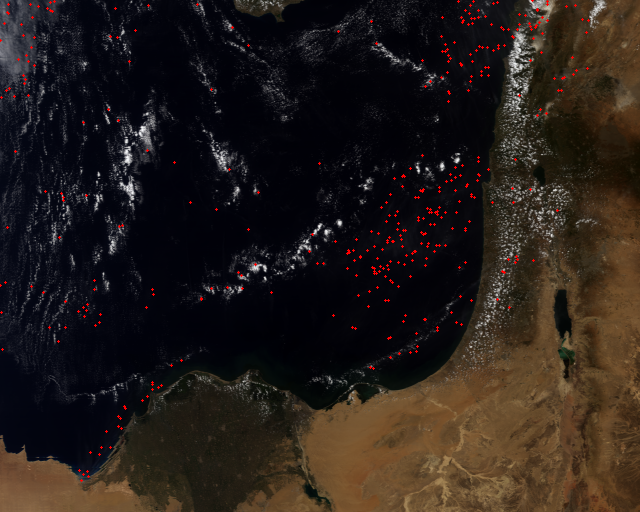
\includegraphics[width=.3\paperwidth]{figs/masks/cmask_samples_km_KM4_TC.png}
            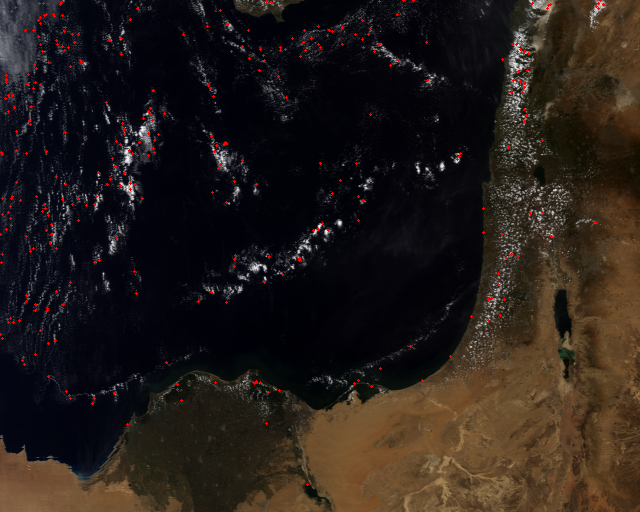
\includegraphics[width=.3\paperwidth]{figs/masks/cmask_samples_km_KM3_TC.png}
        }

        \vspace{.2em}

        \makebox[\textwidth]{
            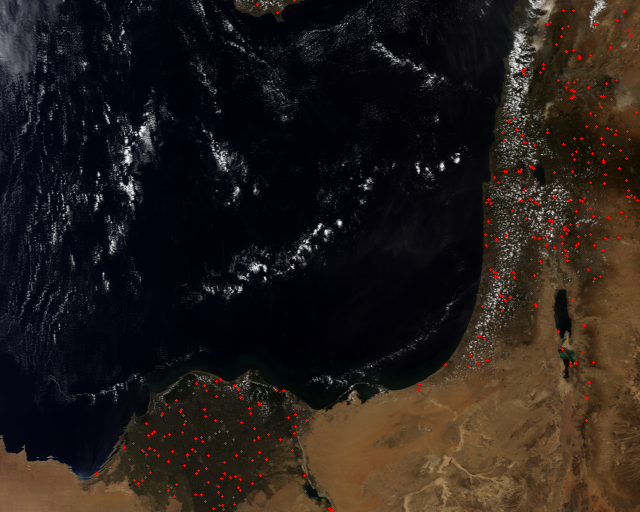
\includegraphics[width=.3\paperwidth]{figs/masks/cmask_samples_km_KM1_TC.png}
            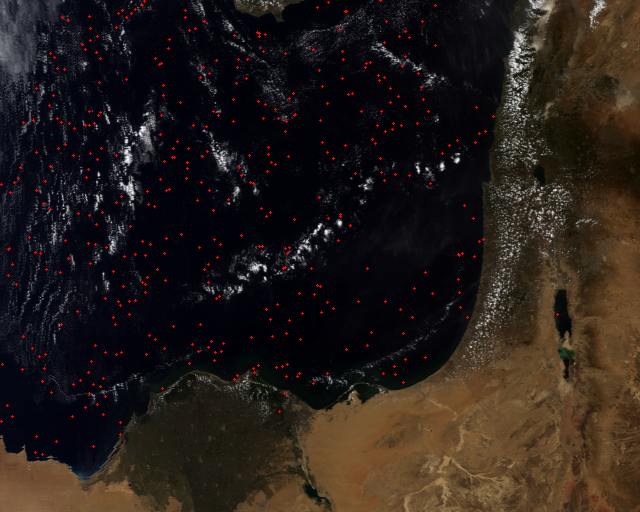
\includegraphics[width=.3\paperwidth]{figs/masks/cmask_samples_km_KM2_TC.png}
            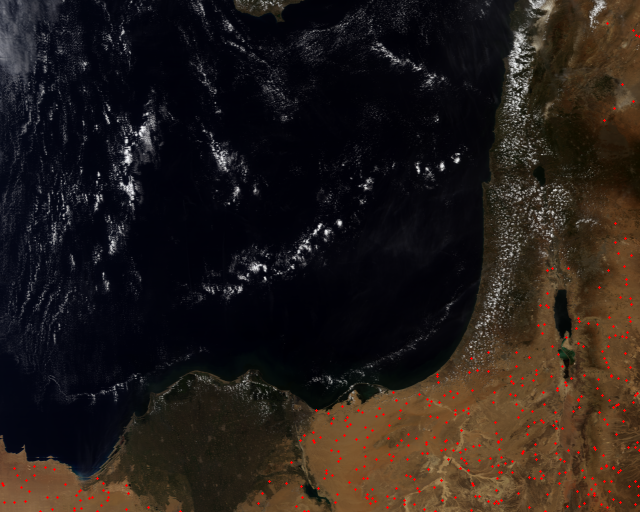
\includegraphics[width=.3\paperwidth]{figs/masks/cmask_samples_km_KM5_TC.png}
        }
    \end{center}

    \caption{Pixels chosen from K-means masks for each class as samples for supervised maximum-likelihood classification. Top: KM4 (ice cloud), KM3 (water cloud). Bottom: KM1 (vegetation), KM2 (water), KM5 (arid)}
    \label{thresh_samples}
\end{figure}

\begin{figure}[h!]
    \centering
    \begin{tabular}{c|cccccc}
    & KM1 & KM2 & KM3 & KM4 & KM5 \\
    \hline
    Pixel Count & 398 & 400 & 396 & 397 & 397\\
    Area (km$^2$) & 485 & 747 & 846 & 609 & 497\\
    \end{tabular}
    \caption{Area and quantity of samples chosen from K-means pixel classes.}
    \label{sample_km_areas}
\end{figure}

\clearpage

\begin{figure}[h!]
    \centering

    \begin{center}
        \makebox[\textwidth]{
            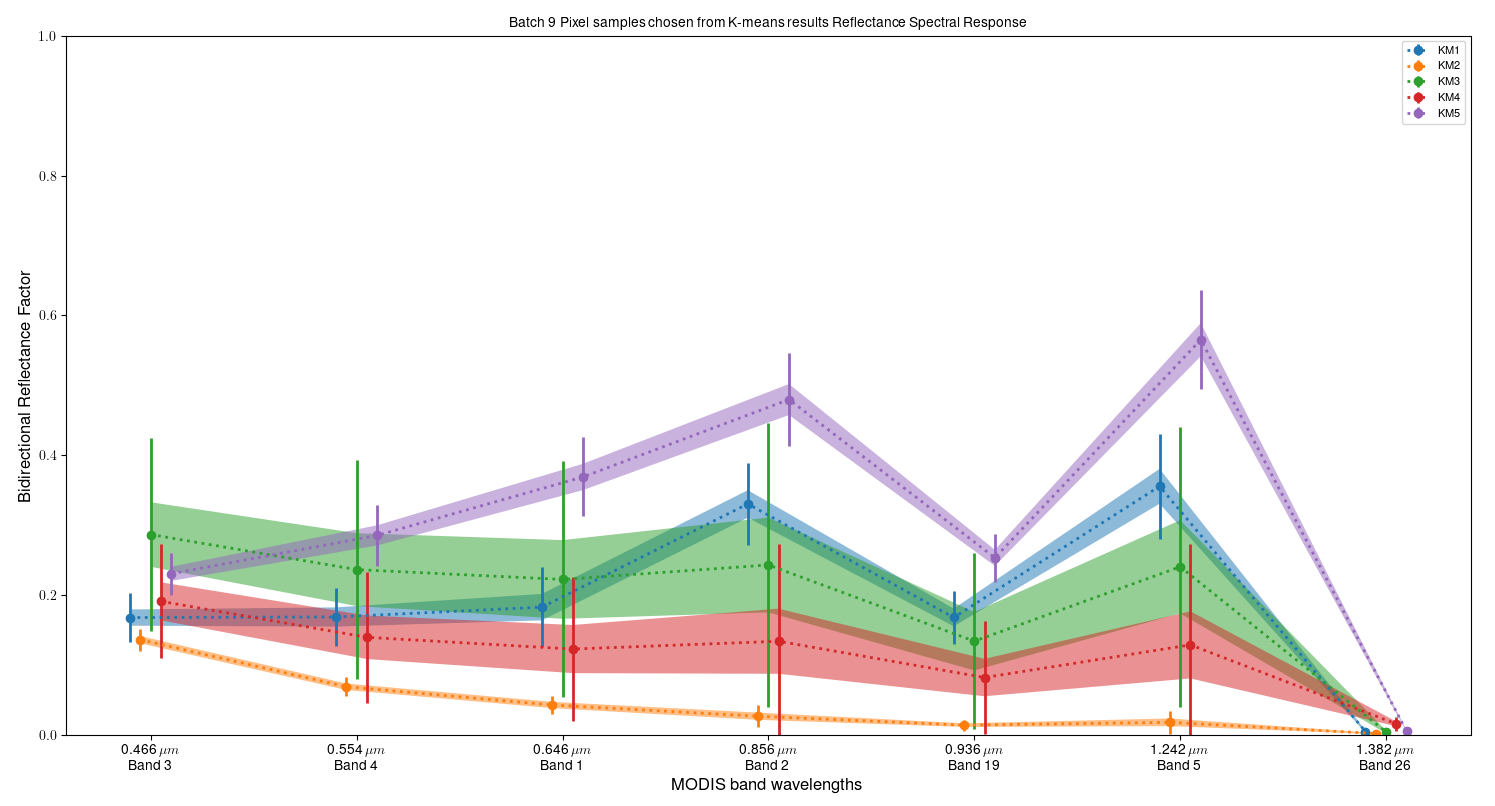
\includegraphics[width=.85\paperwidth]{figs/spectra/ref_samples_km_b9_cropped.png}
        }
        \makebox[\textwidth]{
            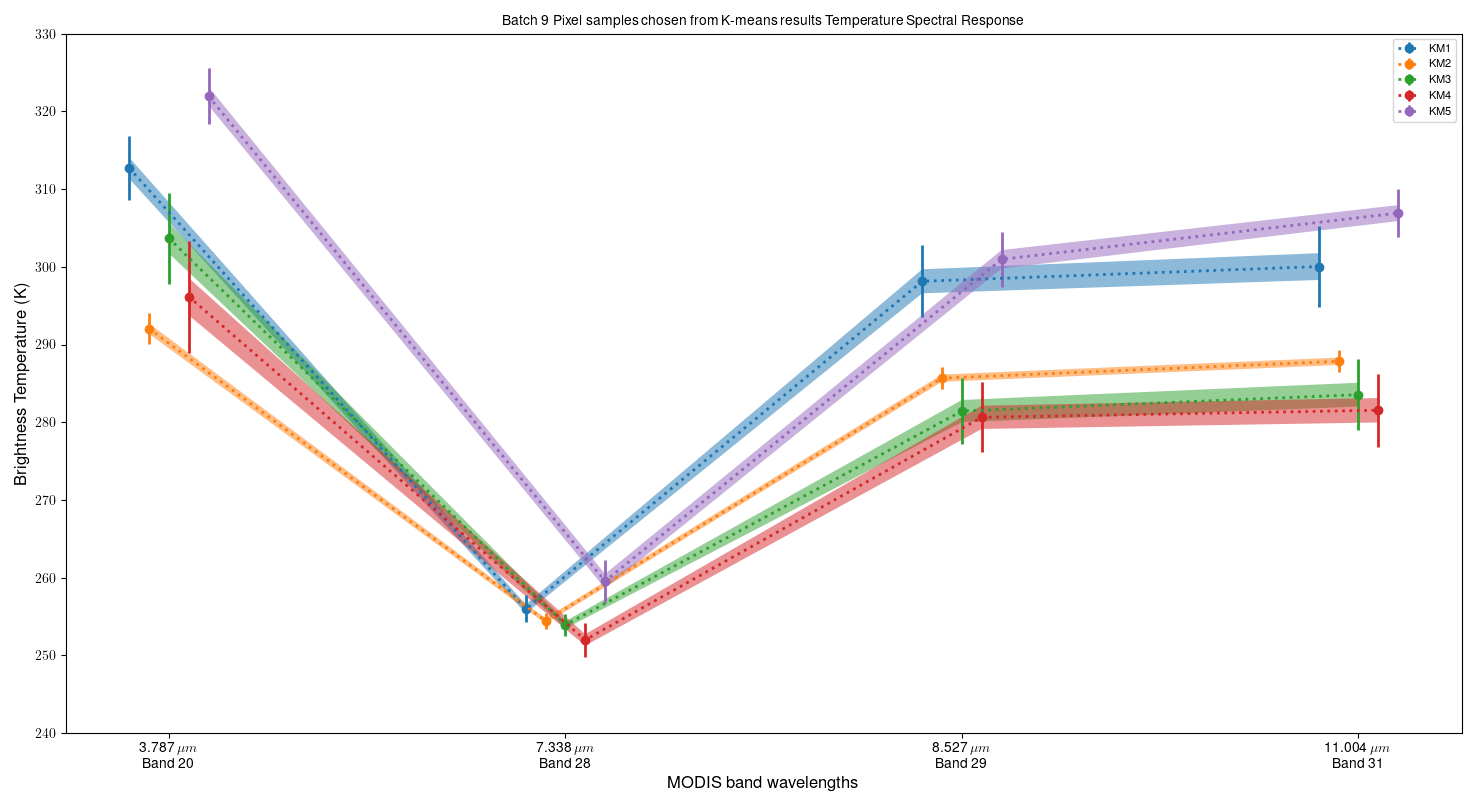
\includegraphics[width=.85\paperwidth]{figs/spectra/temp_samples_km_b9_cropped.png}
        }
    \end{center}

    \caption{}
    \label{mlc_thresh_spectra}
\end{figure}



\clearpage

\begin{figure}[h!]
\centering
\begin{tabular}{C|C|C|CCCCCCC}

\lambda & \mu & \sigma & \multicolumn{7}{c}{Reflectance Covariance $(\times10^{4})$} \\

\hline
\multicolumn{10}{c}{KM1} \\
\hline
0.466 & 0.168 & 0.035 & 12.2 & 13.5 & 15.3 & 11.1 & 6.2 & 15.0 & 0.6 \\
0.554 & 0.169 & 0.041 & 13.5 & 17.0 & 21.8 & 15.5 & 9.9 & 21.9 & 0.9 \\
0.646 & 0.183 & 0.057 & 15.3 & 21.8 & 32.2 & 20.5 & 14.8 & 31.5 & 1.6 \\
0.856 & 0.331 & 0.059 & 11.1 & 15.5 & 20.5 & 34.8 & 19.4 & 41.1 & 1.1 \\
0.936 & 0.168 & 0.038 & 6.2 & 9.9 & 14.8 & 19.4 & 14.5 & 25.1 & 1.2 \\
1.242 & 0.356 & 0.075 & 15.0 & 21.9 & 31.5 & 41.1 & 25.1 & 56.1 & 1.8 \\
1.382 & 0.005 & 0.005 & 0.6 & 0.9 & 1.6 & 1.1 & 1.2 & 1.8 & 0.3 \\

\hline
\multicolumn{10}{c}{KM2} \\
\hline
0.466 & 0.043 & 0.013 & 1.8 & 2.1 & 1.7 & 1.8 & 2.1 & 1.0 & 0.0 \\
0.554 & 0.027 & 0.016 & 2.1 & 2.4 & 1.7 & 2.0 & 2.5 & 1.2 & 0.0 \\
0.646 & 0.136 & 0.016 & 1.7 & 1.7 & 2.4 & 1.8 & 1.7 & 0.8 & -0.0 \\
0.856 & 0.069 & 0.014 & 1.8 & 2.0 & 1.8 & 1.9 & 2.0 & 0.9 & 0.0 \\
0.936 & 0.018 & 0.016 & 2.1 & 2.5 & 1.7 & 2.0 & 2.7 & 1.2 & 0.1 \\
1.242 & 0.014 & 0.008 & 1.0 & 1.2 & 0.8 & 0.9 & 1.2 & 0.6 & 0.1 \\
1.382 & 0.002 & 0.002 & 0.0 & 0.0 & -0.0 & 0.0 & 0.1 & 0.1 & 0.1 \\

\hline
\multicolumn{10}{c}{KM3} \\
\hline
0.466 & 0.223 & 0.169 & 285.6 & 341.1 & 232.2 & 264.5 & 326.0 & 208.9 & 7.0 \\
0.554 & 0.243 & 0.203 & 341.1 & 414.5 & 275.0 & 315.6 & 400.5 & 254.1 & 8.6 \\
0.646 & 0.287 & 0.138 & 232.2 & 275.0 & 192.0 & 215.8 & 262.9 & 167.8 & 5.3 \\
0.856 & 0.237 & 0.156 & 264.5 & 315.6 & 215.8 & 245.4 & 301.4 & 193.1 & 6.4 \\
0.936 & 0.241 & 0.200 & 326.0 & 400.5 & 262.9 & 301.4 & 400.4 & 245.6 & 8.2 \\
1.242 & 0.134 & 0.125 & 208.9 & 254.1 & 167.8 & 193.1 & 245.6 & 157.8 & 5.7 \\
1.382 & 0.005 & 0.006 & 7.0 & 8.6 & 5.3 & 6.4 & 8.2 & 5.7 & 0.4 \\

\hline
\multicolumn{10}{c}{KM4} \\
\hline
0.466 & 0.123 & 0.103 & 107.0 & 139.1 & 80.3 & 96.2 & 137.9 & 78.5 & -0.4 \\
0.554 & 0.134 & 0.140 & 139.1 & 195.4 & 98.3 & 123.4 & 197.9 & 111.2 & 0.6 \\
0.646 & 0.191 & 0.082 & 80.3 & 98.3 & 66.7 & 74.4 & 97.7 & 54.4 & -1.2 \\
0.856 & 0.140 & 0.093 & 96.2 & 123.4 & 74.4 & 87.4 & 122.3 & 69.2 & -0.6 \\
0.936 & 0.129 & 0.144 & 137.9 & 197.9 & 97.7 & 122.3 & 207.7 & 112.5 & 0.8 \\
1.242 & 0.082 & 0.080 & 78.5 & 111.2 & 54.4 & 69.2 & 112.5 & 64.7 & 1.1 \\
1.382 & 0.016 & 0.010 & -0.4 & 0.6 & -1.2 & -0.6 & 0.8 & 1.1 & 1.0 \\

\hline
\multicolumn{10}{c}{KM5} \\
\hline
0.466 & 0.369 & 0.057 & 32.1 & 36.7 & 14.8 & 23.6 & 36.3 & 11.7 & -0.3 \\
0.554 & 0.480 & 0.067 & 36.7 & 44.4 & 16.9 & 26.9 & 44.4 & 13.0 & -0.5 \\
0.646 & 0.231 & 0.030 & 14.8 & 16.9 & 9.2 & 12.5 & 16.3 & 4.1 & -0.2 \\
0.856 & 0.286 & 0.043 & 23.6 & 26.9 & 12.5 & 18.8 & 26.2 & 8.1 & -0.3 \\
0.936 & 0.565 & 0.071 & 36.3 & 44.4 & 16.3 & 26.2 & 50.4 & 13.4 & -0.6 \\
1.242 & 0.253 & 0.035 & 11.7 & 13.0 & 4.1 & 8.1 & 13.4 & 12.0 & 0.4 \\
1.382 & 0.005 & 0.004 & -0.3 & -0.5 & -0.2 & -0.3 & -0.6 & 0.4 & 0.1 \\

\end{tabular}
\caption{samples km reflectance statistics}
\label{samples_km_ref_stats}
\end{figure}

\clearpage

\begin{figure}[h!]
\centering
\begin{tabular}{C|C|C|CCCC}

\lambda & \mu & \sigma & \multicolumn{4}{c}{Brightness Temp. Covariance $(\times10^{2})$} \\

\hline
\multicolumn{7}{c}{KM1} \\
\hline
3.79 & 312.7 & 4.10 & 1685.3 & 314.2 & 1303.2 & 1523.8 \\
7.34 & 256.0 & 1.73 & 314.2 & 300.9 & 410.4 & 525.2 \\
8.53 & 298.1 & 4.64 & 1303.2 & 410.4 & 2158.9 & 2360.5 \\
11.00 & 300.0 & 5.18 & 1523.8 & 525.2 & 2360.5 & 2689.2 \\

\hline
\multicolumn{7}{c}{KM2} \\
\hline
3.79 & 292.0 & 2.01 & 406.1 & 58.5 & 89.6 & 76.4 \\
7.34 & 254.5 & 1.06 & 58.5 & 112.2 & 96.9 & 89.4 \\
8.53 & 285.7 & 1.41 & 89.6 & 96.9 & 198.8 & 194.2 \\
11.00 & 287.8 & 1.43 & 76.4 & 89.4 & 194.2 & 205.7 \\

\hline
\multicolumn{7}{c}{KM3} \\
\hline
3.79 & 303.7 & 5.85 & 3428.4 & 103.2 & -941.2 & -1023.6 \\
7.34 & 253.9 & 1.42 & 103.2 & 202.4 & 354.6 & 382.2 \\
8.53 & 281.4 & 4.28 & -941.2 & 354.6 & 1836.7 & 1961.1 \\
11.00 & 283.6 & 4.60 & -1023.6 & 382.2 & 1961.1 & 2123.0 \\

\hline
\multicolumn{7}{c}{KM4} \\
\hline
3.79 & 296.2 & 7.20 & 5201.2 & 533.0 & -853.1 & -646.2 \\
7.34 & 252.0 & 2.21 & 533.0 & 489.8 & 455.0 & 599.3 \\
8.53 & 280.6 & 4.49 & -853.1 & 455.0 & 2019.8 & 2082.2 \\
11.00 & 281.5 & 4.72 & -646.2 & 599.3 & 2082.2 & 2234.2 \\

\hline
\multicolumn{7}{c}{KM5} \\
\hline
3.79 & 322.0 & 3.63 & 1321.8 & 270.2 & -203.2 & 767.7 \\
7.34 & 259.5 & 2.79 & 270.2 & 782.2 & 489.4 & 516.5 \\
8.53 & 301.0 & 3.56 & -203.2 & 489.4 & 1270.3 & 480.4 \\
11.00 & 306.9 & 3.08 & 767.7 & 516.5 & 480.4 & 953.2 \\

\end{tabular}
\caption{samples km brightness temp. statistics}
\label{samples_km_temp_stats}
\end{figure}


\clearpage

\section{Maximum-likelihood classification with K-means samples}

\begin{figure}[h!]
    \centering

    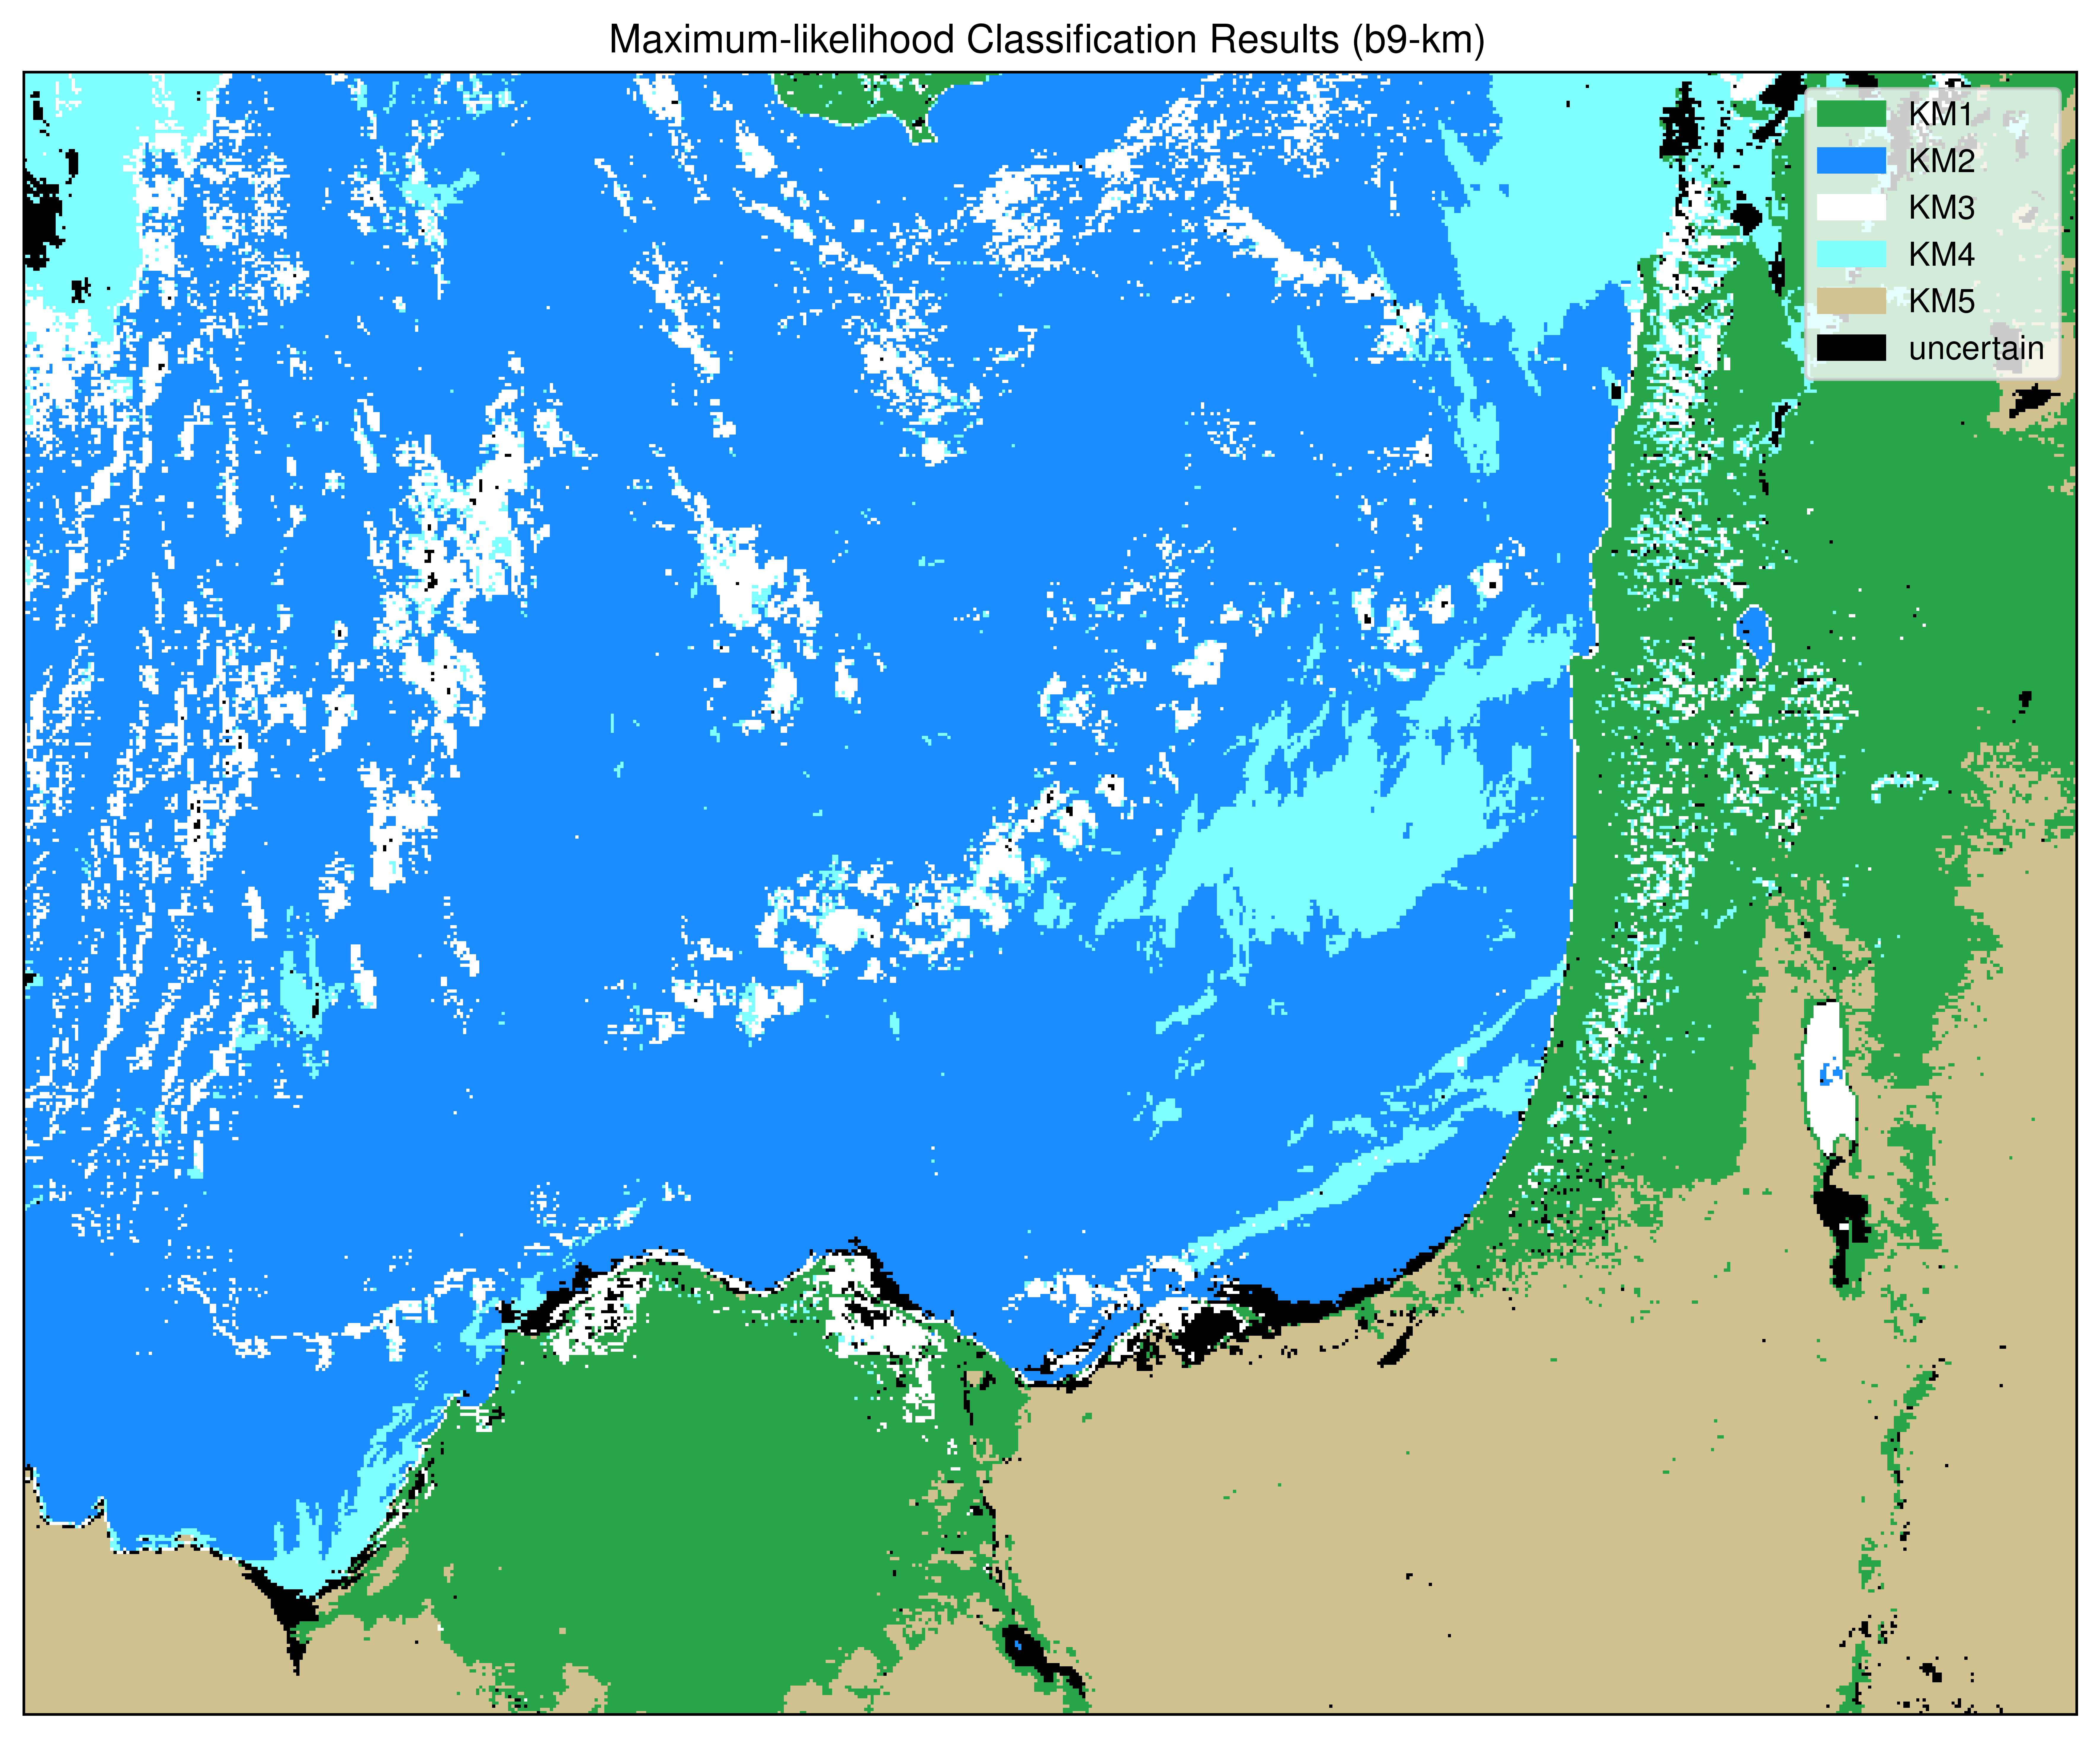
\includegraphics[width=.85\textwidth]{figs/class/mlc_b9-km_6c.png}

    \caption{}
    \label{mlc_km_results}
\end{figure}


\begin{figure}[h!]
    \centering
    \begin{tabular}{c|ccccccc}
    & KM1 & KM2 & KM3 & KM4 & KM5 & Uncertain\\
    \hline
    Pixel Count & 58435 & 155717 & 24430 & 22898 & 61084 & 5116\\
    Area (km$^2$) & 71943 & 287288 & 49023 & 35537 & 77089 & 7806\\
    \end{tabular}
    \caption{Area and quantity of pixel classes from maximum-likelihood classification using K-means samples chosen from K-means classes.}
    \label{mlc_km_areas}
\end{figure}


\clearpage

\begin{figure}[h!]
\centering
\begin{tabular}{C|C|C|CCCCCCC}

\lambda & \mu & \sigma & \multicolumn{7}{c}{Reflectance Covariance $(\times10^{4})$} \\

\hline
\multicolumn{10}{c}{KM1} \\
\hline
0.466 & 0.167 & 0.033 & 10.7 & 12.0 & 14.4 & 10.9 & 5.6 & 15.0 & 0.5 \\
0.554 & 0.169 & 0.040 & 12.0 & 15.9 & 21.7 & 16.4 & 9.8 & 23.3 & 0.8 \\
0.646 & 0.184 & 0.058 & 14.4 & 21.7 & 33.4 & 22.2 & 15.2 & 34.1 & 1.3 \\
0.856 & 0.335 & 0.059 & 10.9 & 16.4 & 22.2 & 34.8 & 18.5 & 41.7 & 0.7 \\
0.936 & 0.170 & 0.037 & 5.6 & 9.8 & 15.2 & 18.5 & 13.7 & 24.2 & 1.0 \\
1.242 & 0.362 & 0.076 & 15.0 & 23.3 & 34.1 & 41.7 & 24.2 & 57.2 & 1.3 \\
1.382 & 0.005 & 0.005 & 0.5 & 0.8 & 1.3 & 0.7 & 1.0 & 1.3 & 0.3 \\

\hline
\multicolumn{10}{c}{KM2} \\
\hline
0.466 & 0.042 & 0.013 & 1.6 & 1.7 & 1.6 & 1.6 & 1.9 & 0.8 & 0.0 \\
0.554 & 0.026 & 0.014 & 1.7 & 2.0 & 1.6 & 1.6 & 2.1 & 1.0 & 0.1 \\
0.646 & 0.136 & 0.016 & 1.6 & 1.6 & 2.5 & 1.8 & 1.7 & 0.7 & -0.1 \\
0.856 & 0.068 & 0.013 & 1.6 & 1.6 & 1.8 & 1.7 & 1.8 & 0.8 & 0.0 \\
0.936 & 0.018 & 0.015 & 1.9 & 2.1 & 1.7 & 1.8 & 2.4 & 1.1 & 0.1 \\
1.242 & 0.014 & 0.007 & 0.8 & 1.0 & 0.7 & 0.8 & 1.1 & 0.5 & 0.1 \\
1.382 & 0.003 & 0.003 & 0.0 & 0.1 & -0.1 & 0.0 & 0.1 & 0.1 & 0.1 \\

\hline
\multicolumn{10}{c}{KM3} \\
\hline
0.466 & 0.206 & 0.147 & 216.6 & 262.0 & 180.4 & 200.1 & 263.1 & 154.1 & 3.8 \\
0.554 & 0.223 & 0.179 & 262.0 & 321.7 & 216.0 & 241.6 & 324.2 & 190.0 & 4.9 \\
0.646 & 0.272 & 0.124 & 180.4 & 216.0 & 152.9 & 167.1 & 216.4 & 126.3 & 2.9 \\
0.856 & 0.221 & 0.136 & 200.1 & 241.6 & 167.1 & 185.1 & 242.2 & 141.9 & 3.4 \\
0.936 & 0.224 & 0.182 & 263.1 & 324.2 & 216.4 & 242.2 & 331.2 & 191.9 & 5.0 \\
1.242 & 0.120 & 0.107 & 154.1 & 190.0 & 126.3 & 141.9 & 191.9 & 113.8 & 3.2 \\
1.382 & 0.003 & 0.005 & 3.8 & 4.9 & 2.9 & 3.4 & 5.0 & 3.2 & 0.2 \\

\hline
\multicolumn{10}{c}{KM4} \\
\hline
0.466 & 0.120 & 0.089 & 79.9 & 114.6 & 58.7 & 71.7 & 121.9 & 66.7 & -0.1 \\
0.554 & 0.132 & 0.132 & 114.6 & 175.4 & 78.7 & 101.5 & 187.5 & 101.2 & 0.1 \\
0.646 & 0.190 & 0.070 & 58.7 & 78.7 & 48.8 & 54.6 & 83.8 & 45.9 & -0.5 \\
0.856 & 0.138 & 0.081 & 71.7 & 101.5 & 54.6 & 65.2 & 108.0 & 59.0 & -0.2 \\
0.936 & 0.131 & 0.142 & 121.9 & 187.5 & 83.8 & 108.0 & 202.1 & 108.0 & -0.1 \\
1.242 & 0.084 & 0.077 & 66.7 & 101.2 & 45.9 & 59.0 & 108.0 & 59.3 & 0.6 \\
1.382 & 0.018 & 0.009 & -0.1 & 0.1 & -0.5 & -0.2 & -0.1 & 0.6 & 0.9 \\

\hline
\multicolumn{10}{c}{KM5} \\
\hline
0.466 & 0.367 & 0.054 & 29.6 & 34.7 & 13.9 & 22.0 & 35.2 & 10.4 & -0.4 \\
0.554 & 0.476 & 0.065 & 34.7 & 42.3 & 16.3 & 25.6 & 43.6 & 11.9 & -0.6 \\
0.646 & 0.229 & 0.029 & 13.9 & 16.3 & 8.5 & 11.7 & 16.4 & 3.7 & -0.3 \\
0.856 & 0.283 & 0.042 & 22.0 & 25.6 & 11.7 & 17.6 & 25.8 & 7.4 & -0.4 \\
0.936 & 0.562 & 0.071 & 35.2 & 43.6 & 16.4 & 25.8 & 51.1 & 13.0 & -0.5 \\
1.242 & 0.251 & 0.033 & 10.4 & 11.9 & 3.7 & 7.4 & 13.0 & 11.0 & 0.4 \\
1.382 & 0.005 & 0.003 & -0.4 & -0.6 & -0.3 & -0.4 & -0.5 & 0.4 & 0.1 \\

\end{tabular}
\caption{mlc km reflectance statistics}
\label{mlc_km_ref_stats}
\end{figure}

\clearpage

\begin{figure}[h!]
\centering
\begin{tabular}{C|C|C|CCCC}

\lambda & \mu & \sigma & \multicolumn{4}{c}{Brightness Temp. Covariance $(\times10^{2})$} \\

\hline
\multicolumn{7}{c}{KM1} \\
\hline
3.79 & 312.7 & 4.55 & 2073.3 & 447.9 & 1684.4 & 1947.3 \\
7.34 & 255.9 & 1.76 & 447.9 & 308.2 & 541.8 & 657.6 \\
8.53 & 298.2 & 4.81 & 1684.4 & 541.8 & 2317.0 & 2579.9 \\
11.00 & 300.1 & 5.44 & 1947.3 & 657.6 & 2579.9 & 2957.5 \\

\hline
\multicolumn{7}{c}{KM2} \\
\hline
3.79 & 291.9 & 1.68 & 281.2 & 26.2 & 16.1 & 2.0 \\
7.34 & 254.3 & 1.12 & 26.2 & 126.0 & 104.7 & 102.4 \\
8.53 & 285.5 & 1.33 & 16.1 & 104.7 & 176.4 & 178.0 \\
11.00 & 287.6 & 1.42 & 2.0 & 102.4 & 178.0 & 201.0 \\

\hline
\multicolumn{7}{c}{KM3} \\
\hline
3.79 & 303.6 & 5.89 & 3464.0 & 22.8 & -1246.9 & -1344.6 \\
7.34 & 254.3 & 1.32 & 22.8 & 173.9 & 311.9 & 317.7 \\
8.53 & 282.5 & 4.08 & -1246.9 & 311.9 & 1663.4 & 1712.0 \\
11.00 & 284.7 & 4.23 & -1344.6 & 317.7 & 1712.0 & 1787.1 \\

\hline
\multicolumn{7}{c}{KM4} \\
\hline
3.79 & 296.6 & 7.48 & 5598.9 & 742.4 & -849.9 & -645.4 \\
7.34 & 251.6 & 2.27 & 742.4 & 514.4 & 530.5 & 680.7 \\
8.53 & 279.6 & 5.29 & -849.9 & 530.5 & 2798.8 & 2840.6 \\
11.00 & 280.2 & 5.44 & -645.4 & 680.7 & 2840.6 & 2964.9 \\

\hline
\multicolumn{7}{c}{KM5} \\
\hline
3.79 & 321.9 & 3.61 & 1302.8 & 265.5 & -195.0 & 753.4 \\
7.34 & 259.5 & 2.65 & 265.5 & 704.8 & 417.3 & 449.5 \\
8.53 & 301.2 & 3.30 & -195.0 & 417.3 & 1091.7 & 356.6 \\
11.00 & 307.0 & 2.84 & 753.4 & 449.5 & 356.6 & 809.4 \\

\end{tabular}
\caption{mlc km brightness temp. statistics}
\label{mlc_km_temp_stats}
\end{figure}


\begin{figure}[h!]
\centering
    \begin{center}
        \makebox[\textwidth]{
\begin{tabular}{C|CCCCCC|C}
& \textnormal{KM1} & \textnormal{KM2} & \textnormal{KM3} & \textnormal{KM4} & \textnormal{KM5} & \textnormal{Uncertain} & \textnormal{Cons. Acc.} \\
\hline
\textnormal{MLC1} & 375 & 0 & 2 & 6 & 9 & 6 & 0.942 \\
\textnormal{MLC2} & 0 & 384 & 13 & 1 & 0 & 2 & 0.960 \\
\textnormal{MLC3} & 6 & 16 & 337 & 23 & 0 & 14 & 0.851 \\
\textnormal{MLC4} & 6 & 104 & 48 & 219 & 0 & 20 & 0.552 \\
\textnormal{MLC5} & 11 & 0 & 0 & 0 & 383 & 3 & 0.965 \\
\hline
\textnormal{Prod. Acc.} & 0.942 & 0.762 & 0.843 & 0.880 & 0.977\\
\end{tabular}
        }
    \end{center}
\caption{samples km/mlc km confusion matrix}
\label{confusion_samples_km-mlc_km}
\end{figure}

\clearpage

\begin{figure}[h!]
\centering
\begin{tabular}{C|C|C|CCCCCCC}

\lambda & \mu & \sigma & \multicolumn{7}{c}{Reflectance Covariance $(\times10^{4})$} \\
\hline0.466 & 0.235 & 0.168 & 282.5 & 334.6 & 210.9 & 235.9 & 318.1 & 201.4 & 7.8 \\
0.554 & 0.277 & 0.210 & 334.6 & 439.3 & 235.1 & 270.2 & 433.1 & 259.2 & 11.8 \\
0.646 & 0.244 & 0.137 & 210.9 & 235.1 & 187.2 & 191.6 & 214.0 & 148.8 & 7.0 \\
0.856 & 0.236 & 0.144 & 235.9 & 270.2 & 191.6 & 206.6 & 249.6 & 165.6 & 6.6 \\
0.936 & 0.272 & 0.216 & 318.1 & 433.1 & 214.0 & 249.6 & 467.5 & 254.2 & 12.2 \\
1.242 & 0.157 & 0.127 & 201.4 & 259.2 & 148.8 & 165.6 & 254.2 & 161.3 & 9.1 \\
1.382 & 0.014 & 0.015 & 7.8 & 11.8 & 7.0 & 6.6 & 12.2 & 9.1 & 2.2 \\

\end{tabular}
\begin{tabular}{C|C|C|CCCC}

\lambda & \mu & \sigma & \multicolumn{4}{c}{Brightness Temp. Covariance $(\times10^{2})$} \\
\hline3.79 & 304.2 & 10.11 & 10215.1 & 1242.3 & 4219.0 & 5408.5 \\
7.34 & 254.3 & 4.13 & 1242.3 & 1706.9 & 3105.3 & 3723.4 \\
8.53 & 286.3 & 11.10 & 4219.0 & 3105.3 & 12328.1 & 13482.3 \\
11.00 & 288.5 & 12.30 & 5408.5 & 3723.4 & 13482.3 & 15132.9 \\

\end{tabular}
\caption{mlc km Uncertain reflectance and brightness temp. statistics}
\label{mlc_km_unc_stats}
\end{figure}

\bibliography{main}
%\printbibliography

\end{document}
